\documentclass[12pt,twoside]{article}


\newcommand{\reporttitle}{Optimising post-trade processing using  Distributed Ledger Technology}
\newcommand{\reportsubtitle}{Can Distributed Ledger Technology save the financial world time and money?}
\newcommand{\reportauthor}{Michael Carneciu}
\newcommand{\reporttype}{BEng Individual Project}
\newcommand{\cid}{09...}

% include files that load packages and define macros
%%%%%%%%%%%%%%%%%%%%%%%%%%%%%%%%%%%%%%%%%
% University Assignment Title Page 
% LaTeX Template
% Version 1.0 (27/12/12)
%
% This template has been downloaded from:
% http://www.LaTeXTemplates.com
%
% Original author:
% WikiBooks (http://en.wikibooks.org/wiki/LaTeX/Title_Creation)
%
% License:
% CC BY-NC-SA 3.0 (http://creativecommons.org/licenses/by-nc-sa/3.0/)
% 
% Instructions for using this template:
% This title page is capable of being compiled as is. This is not useful for 
% including it in another document. To do this, you have two options: 
%
% 1) Copy/paste everything between \begin{document} and \end{document} 
% starting at \begin{titlepage} and paste this into another LaTeX file where you 
% want your title page.
% OR
% 2) Remove everything outside the \begin{titlepage} and \end{titlepage} and 
% move this file to the same directory as the LaTeX file you wish to add it to. 
% Then add \input{./title_page_1.tex} to your LaTeX file where you want your
% title page.
%
%----------------------------------------------------------------------------------------
%	PACKAGES AND OTHER DOCUMENT CONFIGURATIONS
%----------------------------------------------------------------------------------------
\usepackage[table,xcdraw]{xcolor}
\usepackage{ifxetex}
\usepackage{textpos}
\usepackage[numbers]{natbib}
\usepackage{kpfonts}
\usepackage[a4paper,hmargin=2.8cm,vmargin=2.0cm,includeheadfoot]{geometry}
\usepackage{ifxetex}
\usepackage{stackengine}
\usepackage{tabularx,longtable,multirow,caption}%hangcaption
\usepackage{fncylab} %formatting of labels
\usepackage{fancyhdr}
\usepackage{color}
\usepackage[tight,ugly]{units}
\usepackage{float}
\usepackage[english]{babel}
\usepackage{amsmath}
\usepackage{graphicx}
\usepackage[colorinlistoftodos]{todonotes}
\usepackage{dsfont}
\usepackage{epstopdf} % automatically replace .eps with .pdf in graphics
\usepackage{natbib}
\usepackage{array}
\usepackage{latexsym}
\usepackage{etoolbox}
\usepackage[hyphenbreaks]{breakurl}
\usepackage[hyphens]{url}
\usepackage{enumerate} % for numbering with [a)] format 
\usepackage{subcaption}
\usepackage{smartdiagram}
\usepackage{booktabs}

%\documentclass[xcolor=table]{beamer}

\ifxetex
\usepackage{fontspec}
\setmainfont[Scale=.8]{OpenDyslexic-Regular}
\else
\usepackage[pdftex,hypertexnames=false,colorlinks]{hyperref} % provide links in pdf
\hypersetup{pdftitle={},
  pdfsubject={}, 
  pdfauthor={\reportauthor},
  pdfkeywords={}, 
  pdfstartview=FitH,
  pdfpagemode={UseOutlines},% None, FullScreen, UseOutlines
  bookmarksnumbered=true, bookmarksopen=true, colorlinks,
    citecolor=black,%
    filecolor=black,%
    linkcolor=black,%
    urlcolor=black}
\usepackage[all]{hypcap}
\fi

\usepackage{tcolorbox}

% various theorems
\usepackage{ntheorem}
\theoremstyle{break}
\newtheorem{lemma}{Lemma}
\newtheorem{theorem}{Theorem}
\newtheorem{remark}{Remark}
\newtheorem{definition}{Definition}
\newtheorem{proof}{Proof}

% example-environment
\newenvironment{example}[1][]
{ 
\vspace{4mm}
\noindent\makebox[\linewidth]{\rule{\hsize}{1.5pt}}
\textbf{Example #1}\\
}
{ 
\noindent\newline\makebox[\linewidth]{\rule{\hsize}{1.0pt}}
}



%\renewcommand{\rmdefault}{pplx} % Palatino
% \renewcommand{\rmdefault}{put} % Utopia

\ifxetex
\else
\renewcommand*{\rmdefault}{bch} % Charter
\renewcommand*{\ttdefault}{cmtt} % Computer Modern Typewriter
%\renewcommand*{\rmdefault}{phv} % Helvetica
%\renewcommand*{\rmdefault}{iwona} % Avant Garde
\fi

\setlength{\parindent}{0em}  % indentation of paragraph

\setlength{\headheight}{14.5pt}
\pagestyle{fancy}
\fancyfoot[ER,OL]{\thepage}%Page no. in the left on
                                %odd pages and on right on even pages
\fancyfoot[OC,EC]{\sffamily }
\renewcommand{\headrulewidth}{0.1pt}
\renewcommand{\footrulewidth}{0.1pt}
\captionsetup{margin=10pt,font=small,labelfont=bf}


%--- chapter heading

\def\@makechapterhead#1{%
  \vspace*{10\p@}%
  {\parindent \z@ \raggedright %\sffamily
        %{\Large \MakeUppercase{\@chapapp} \space \thechapter}
        %\\
        %\hrulefill
        %\par\nobreak
        %\vskip 10\p@
    \interlinepenalty\@M
    \Huge \bfseries 
    \thechapter \space\space #1\par\nobreak
    \vskip 30\p@
  }}

%---chapter heading for \chapter*  
\def\@makeschapterhead#1{%
  \vspace*{10\p@}%
  {\parindent \z@ \raggedright
    \sffamily
    \interlinepenalty\@M
    \Huge \bfseries  
    #1\par\nobreak
    \vskip 30\p@
  }}
  



% %%%%%%%%%%%%% boxit
\def\Beginboxit
   {\par
    \vbox\bgroup
	   \hrule
	   \hbox\bgroup
		  \vrule \kern1.2pt %
		  \vbox\bgroup\kern1.2pt
   }

\def\Endboxit{%
			      \kern1.2pt
		       \egroup
		  \kern1.2pt\vrule
		\egroup
	   \hrule
	 \egroup
   }	

\newenvironment{boxit}{\Beginboxit}{\Endboxit}
\newenvironment{boxit*}{\Beginboxit\hbox to\hsize{}}{\Endboxit}



\allowdisplaybreaks

\makeatletter
\newcounter{elimination@steps}
\newcolumntype{R}[1]{>{\raggedleft\arraybackslash$}p{#1}<{$}}
\def\elimination@num@rights{}
\def\elimination@num@variables{}
\def\elimination@col@width{}
\newenvironment{elimination}[4][0]
{
    \setcounter{elimination@steps}{0}
    \def\elimination@num@rights{#1}
    \def\elimination@num@variables{#2}
    \def\elimination@col@width{#3}
    \renewcommand{\arraystretch}{#4}
    \start@align\@ne\st@rredtrue\m@ne
}
{
    \endalign
    \ignorespacesafterend
}
\newcommand{\eliminationstep}[2]
{
    \ifnum\value{elimination@steps}>0\leadsto\quad\fi
    \left[
        \ifnum\elimination@num@rights>0
            \begin{array}
            {@{}*{\elimination@num@variables}{R{\elimination@col@width}}
            |@{}*{\elimination@num@rights}{R{\elimination@col@width}}}
        \else
            \begin{array}
            {@{}*{\elimination@num@variables}{R{\elimination@col@width}}}
        \fi
            #1
        \end{array}
    \right]
    & 
    \begin{array}{l}
        #2
    \end{array}
    &%                                    moved second & here
    \addtocounter{elimination@steps}{1}
}
\makeatother

%% Fast macro for column vectors
\makeatletter  
\def\colvec#1{\expandafter\colvec@i#1,,,,,,,,,\@nil}
\def\colvec@i#1,#2,#3,#4,#5,#6,#7,#8,#9\@nil{% 
  \ifx$#2$ \begin{bmatrix}#1\end{bmatrix} \else
    \ifx$#3$ \begin{bmatrix}#1\\#2\end{bmatrix} \else
      \ifx$#4$ \begin{bmatrix}#1\\#2\\#3\end{bmatrix}\else
        \ifx$#5$ \begin{bmatrix}#1\\#2\\#3\\#4\end{bmatrix}\else
          \ifx$#6$ \begin{bmatrix}#1\\#2\\#3\\#4\\#5\end{bmatrix}\else
            \ifx$#7$ \begin{bmatrix}#1\\#2\\#3\\#4\\#5\\#6\end{bmatrix}\else
              \ifx$#8$ \begin{bmatrix}#1\\#2\\#3\\#4\\#5\\#6\\#7\end{bmatrix}\else
                 \PackageError{Column Vector}{The vector you tried to write is too big, use bmatrix instead}{Try using the bmatrix environment}
              \fi
            \fi
          \fi
        \fi
      \fi
    \fi
  \fi 
}  
\makeatother

\robustify{\colvec}

%%% Local Variables: 
%%% mode: latex
%%% TeX-master: "notes"
%%% End: 
 % various packages needed for maths etc.
% quick way of adding a figure
\newcommand{\fig}[3]{
 \begin{center}
 \scalebox{#3}{\includegraphics[#2]{#1}}
 \end{center}
}

%\newcommand*{\point}[1]{\vec{\mkern0mu#1}}
\newcommand{\ci}[0]{\perp\!\!\!\!\!\perp} % conditional independence
\newcommand{\point}[1]{{#1}} % points 
\renewcommand{\vec}[1]{{\boldsymbol{{#1}}}} % vector
\newcommand{\mat}[1]{{\boldsymbol{{#1}}}} % matrix
\newcommand{\R}[0]{\mathds{R}} % real numbers
\newcommand{\Z}[0]{\mathds{Z}} % integers
\newcommand{\N}[0]{\mathds{N}} % natural numbers
\newcommand{\nat}[0]{\mathds{N}} % natural numbers
\newcommand{\Q}[0]{\mathds{Q}} % rational numbers
\ifxetex
\newcommand{\C}[0]{\mathds{C}} % complex numbers
\else
\newcommand{\C}[0]{\mathds{C}} % complex numbers
\fi
\newcommand{\tr}[0]{\text{tr}} % trace
\renewcommand{\d}[0]{\mathrm{d}} % total derivative
\newcommand{\inv}{^{-1}} % inverse
\newcommand{\id}{\mathrm{id}} % identity mapping
\renewcommand{\dim}{\mathrm{dim}} % dimension
\newcommand{\rank}[0]{\mathrm{rk}} % rank
\newcommand{\determ}[1]{\mathrm{det}(#1)} % determinant
\newcommand{\scp}[2]{\langle #1 , #2 \rangle}
\newcommand{\kernel}[0]{\mathrm{ker}} % kernel/nullspace
\newcommand{\img}[0]{\mathrm{Im}} % image
\newcommand{\idx}[1]{{(#1)}}
\DeclareMathOperator*{\diag}{diag}
\newcommand{\E}{\mathds{E}} % expectation
\newcommand{\var}{\mathds{V}} % variance
\newcommand{\gauss}[2]{\mathcal{N}\big(#1,\,#2\big)} % gaussian distribution N(.,.)
\newcommand{\gaussx}[3]{\mathcal{N}\big(#1\,|\,#2,\,#3\big)} % gaussian distribution N(.|.,.)
\newcommand{\gaussBig}[2]{\mathcal{N}\left(#1,\,#2\right)} % see above, but with brackets that adjust to the height of the arguments
\newcommand{\gaussxBig}[3]{\mathcal{N}\left(#1\,|\,#2,\,#3\right)} % see above, but with brackets that adjust to the height of the arguments
\DeclareMathOperator{\cov}{Cov} % covariance (matrix) 
\ifxetex
\renewcommand{\T}[0]{^\top} % transpose
\else
\newcommand{\T}[0]{^\top}
\fi
% matrix determinant
\newcommand{\matdet}[1]{
\left|
\begin{matrix}
#1
\end{matrix}
\right|
}



%%% various color definitions
\definecolor{darkgreen}{rgb}{0,0.6,0}

\newcommand{\blue}[1]{{\color{blue}#1}}
\newcommand{\red}[1]{{\color{red}#1}}
\newcommand{\green}[1]{{\color{darkgreen}#1}}
\newcommand{\orange}[1]{{\color{orange}#1}}
\newcommand{\magenta}[1]{{\color{magenta}#1}}
\newcommand{\cyan}[1]{{\color{cyan}#1}}


% redefine emph
\renewcommand{\emph}[1]{\blue{\bf{#1}}}

% place a colored box around a character
\gdef\colchar#1#2{%
  \tikz[baseline]{%
  \node[anchor=base,inner sep=2pt,outer sep=0pt,fill = #2!20] {#1};
    }%
}%
 % short-hand notation and macros
\usepackage{verbatim}
\usepackage[official]{eurosym}
\bibstyle{natbib}
\usepackage{hyperref}
\hypersetup{%
  colorlinks=true, 
  breaklinks=true, 
  pagebackref=false
}
\usepackage{listings}
\usepackage{color}
 
\definecolor{codegreen}{rgb}{0,0.6,0}
\definecolor{codegray}{rgb}{0.5,0.5,0.5}
\definecolor{codepurple}{rgb}{0.58,0,0.82}
\definecolor{backcolour}{rgb}{0.9,0.9,0.92}

\lstdefinestyle{mystyle}{
    backgroundcolor=\color{backcolour},   
    commentstyle=\color{codegreen},
    keywordstyle=\color{magenta},
    numberstyle=\tiny\color{codegray},
    stringstyle=\color{codepurple},
    breakatwhitespace=false,         
    breaklines=true,                 
    captionpos=b,                    
    keepspaces=true,                 
    numbers=left,                    
    numbersep=5pt,                  
    showspaces=false,                
    showstringspaces=false,
    showtabs=false,                  
    tabsize=2,
    upquote,
    basicstyle=\footnotesize\ttfamily,
    columns=flexible,
    framextopmargin=50pt
}
 
\lstset{style=mystyle}

\graphicspath{{/Users/mikecar/Desktop/Blockchain-dizzy/imgs/}}
%%%%%%%%%%%%%%%%%%%%%%%%%%%%
\begin{document}
% front page
\pagenumbering{gobble}
% Last modification: 2016-09-29 (Marc Deisenroth)
\begin{titlepage}

\newcommand{\HRule}{\rule{\linewidth}{0.5mm}} % Defines a new command for the horizontal lines, change thickness here


%----------------------------------------------------------------------------------------
%	LOGO SECTION
%----------------------------------------------------------------------------------------

\begin{center} % Center remainder of the page

\includegraphics[width = 11cm]{./figures/imperial}\\[0.5cm] 
\vspace{2.5cm}

%----------------------------------------------------------------------------------------
%	HEADING SECTIONS
%----------------------------------------------------------------------------------------
\textsc{\LARGE \reporttype}\\[1.5cm] 
\textsc{\Large Imperial College London}\\[0.5cm] 
\textsc{\large Department of Computing}\\[0.5cm] 
%----------------------------------------------------------------------------------------
%	TITLE SECTION
%----------------------------------------------------------------------------------------

\HRule \\[0.4cm]
{ \huge \bfseries \reporttitle}\\ % Title of your document
%{ \large \bfseries \reportsubtitle}\\
\HRule \\[1.5cm]
\end{center}
%----------------------------------------------------------------------------------------
%	AUTHOR SECTION
%----------------------------------------------------------------------------------------

%\begin{minipage}{0.4\hsize}

\vspace{1cm}
\begin{minipage}{0.4\hsize}
\flushleft
\textsc{Author:}

Michael Carneciu\\
\end{minipage}
\hfill
\begin{minipage}{0.4\hsize}
\flushright
\textsc{Supervisor:}

Dr Anandha Gopalan\\
\vspace{0.5cm}
\textsc{Second Marker:}

Dr Naranker Dulay
\end{minipage}

\vspace{4cm}
\makeatletter
\begin{center}
\@date 
\end{center}

\vfill % Fill the rest of the page with whitespace



\makeatother


\end{titlepage}


\cleardoublepage
\vspace*{2.5cm}
    \LARGE
    \textbf{Abstract}

\normalsize
 \vspace{3cm}

Distributed ledger technology is enabling institutions to optimise their business flows by automating lengthy processes and reducing the effort of maintaining different financial accounts synchronised across all their contributors. A newly implemented platform based on this is Corda, developed specifically for the banking industry. This project focuses on implementing stock trading on Corda and evaluating whether the system is a feasible solution for commercial deployment. In order to do this, we had to ensure its performance, security and regulation controls are up to the standards required by the industry. Since data is shared on a need-to-know basis, not only are security concerns mitigated, but the scalability of the system is also improved compared to other solutions. Performance-wise, the system is expected to yield more than 80,000 transactions per second which is an appropriate value for the industry. From the point of view of regulation, we explored auditing facilities and evaluated the ways in which the system complies with the current financial laws. 

\vspace{0.5cm}
Besides theoretical analysis of features, we tested the privacy and scalability of the system by implementing two applications for a group of banks distributed over different machines: a virtual marketplace with a graphical interface and one where trades are randomly triggered between participants. These demonstrate the usability of the system, while showcasing the data-sharing principles in practice. Introducing new entities into the marketplace has also been achieved, without adding any latencies to the system. 
\cleardoublepage
\vspace*{2.5cm}
    \LARGE
    \textbf{Acknowledgements}

\normalsize
 \vspace{3cm}

I would like to thank Dr Anandha Gopalan for his invaluable help and support - I feel so fortunate to have been supervised and guided by him throughout this project.

\vspace{0.5cm}
I would also like to thank my friends Dom, Ab, Elias, David and Giacomo for teaching me that the dissertation is not the only important part of a final year student's life, along with my mother and the rest of my family for their encouragement during my \textit{Imperial years}.
\newpage
\tableofcontents
\newpage
%%%%%%%%%%%%%%%%%%%%%%%%%%%% Main document

\pagenumbering{arabic}
\section{Introduction}
\label{sec:Introduction}
\subsection{Motivation}
\label{sub:Motivation}
Time has gradually become one of the most important currencies to humankind \cite{mike}. Fortunately, we now benefit from instant messaging, instant information sharing and high speed digital connections between people which help us save vast amounts of time! However, most of the financial world is stuck in the past. While there have been some revolutionary computational developments meant to enhance user experience, such as digital payments and biometrics\cite{digitalfinance}, the parts that involve the most risk still present huge bottlenecks. One of the reasons for this is the rigidity of the industry with regards to change. Migrations are dangerous considering the fact that banks deal with large sums of money and any weakness in the trading infrastructure could have devastating effects on their operation (record loss, incorrect migration protocols leading to capital loss \cite{bankrisk} or triggering a flash event like the Sterling ``flash crash" from October 2016 \cite{flashcrash}).
\\ \\
For stock trading in particular, processing times have been historically long. Looking as far back as the 1700s, transactions between the London Stock Exchange and the Amsterdam Stock Exchange were performed regularly, but the standard time for a trade to complete was 14 days! Of course, this was due to the lack of technology, so the actual stock certificates and cash had to be transported by horse and ship between the two cities \cite{CHsuperold}. Along with the emergence of technology towards the end of the twentieth century, these processing times were gradually shortened, remaining at a maximum of three days, or T+3 since 1995 (meaning that it takes 3 days from the moment a trade has been initialised to the moment the funds and assets have changed ownership on the ledger - the database documenting all the bank's financial records) \cite{TTimes}. Recently, there has been a push in both Europe and the United States to reduce this even further, to T+2 \cite{newTimes} \cite{newTimesUS}. However, is this enough for the present day?
\\ \\
Besides the latency, the traditional way of performing transactions is also error-prone because of the inevitable human interaction \cite{humanrisk}. Any mistake made when a trade is being performed adds even more delays to the processing time because of the need to cancel, change and reprocess the trade which leads to capital loss. Since both time and money are so valuable to us nowadays, there is a clear need to upgrade the way banks do business. However, to be able to adopt any new methodologies and technologies, these have to be thoroughly analysed to verify they can be held to the standards required by the financial world. Given that the financial industry has been one of the drivers of Computing in the past, with their usage of databases to manage records pushing development in this area, it is time once again for banks to lead the way by implementing and adopting computational solutions to deal with the issues presented.
\\ \\
To better explain the impact of the problems we are currently facing, imagine Alice and Bob who want to perform a very simple trade. Alice has \pounds 200 in her digital wallet and Bob has 20 shares of stock A (each priced at \pounds 10). The two of them want to execute an exchange, Alice buying 10 shares from Bob worth \pounds 100. Now, this transaction would immediately get executed if Alice had enough funds in her wallet, Bob had enough shares and the trade details were correctly matched by our system - which is the case here.
\\ \\
The record of the trade is now available on the ledger for everyone to see. This is graphically depicted in Figure \ref{fig:tradescheme}.
 
\begin{figure}[H]
\centering
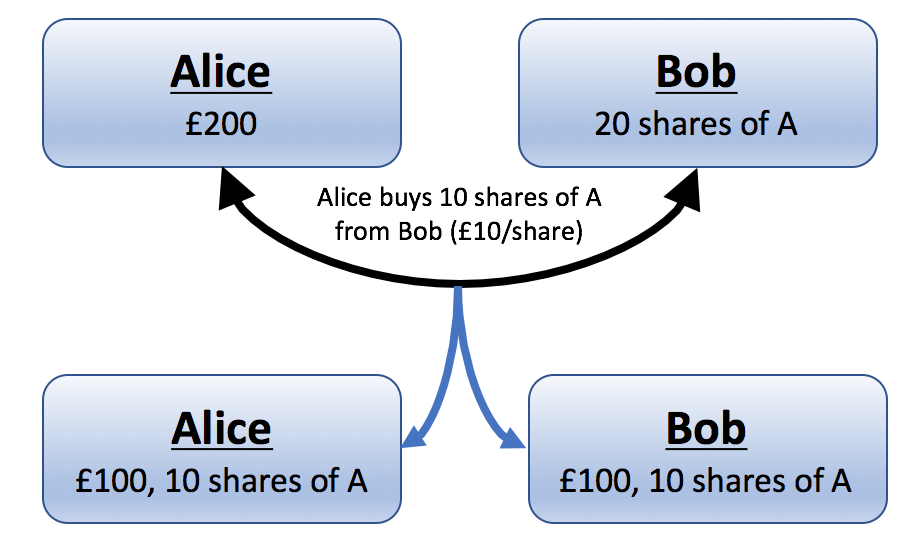
\includegraphics[width=0.7\textwidth]{alicebob.png}
\caption{Simplified schematic representation of a trade}
\centering
\label{fig:tradescheme}
\end{figure}

Since the exchange would be immediate in this ideal system, there are no mistakes that can be done (if the details do not match, the trade is not executed), so once the transaction is triggered it is considered finalised. However, in the real world, the situation is not as simple as here because \textbf{this exchange takes several days}. Trust is crucial when dealing with money and losing it is not an option. 
\\ \\
The bilateral trading ideology, pictured in Figure \ref{fig:bilTrading}, is risky since the counterparties are exposed to risk directly and indirectly, for example if one of them defaults (i.e. has not paid a debt which they are required to have paid \cite{default}). Therefore, there is a need for a \textbf{central counterparty} to mitigate risk in case one of the participants is no longer able to fulfill his promise. Transactions performed on an exchange go through a Clearing House (an intermediary between buyers and sellers of financial instruments) which ensures the parties involved in the trade are able to satisfy their obligations.  Moreover, it helps put all the pieces in place to finalise the transaction, in the process called settlement when the parties' obligations are fulfilled. Due to their nature of managing both sides of a trade, clearing houses also match the highest bidding price to the lowest selling price \cite{exchsettle}. The position of a clearing house in the trading world is depicted in Figure \ref{fig:CCP}. \\ \\
\begin{figure}[H]
    \centering
    \begin{subfigure}[b]{0.48\textwidth}
        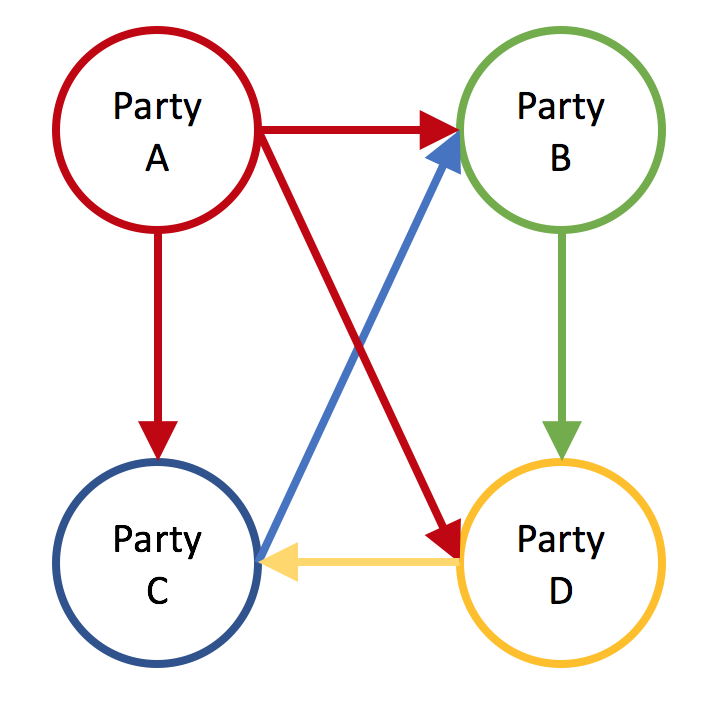
\includegraphics[width=\textwidth]{bilateral.png}
        \caption{Bilateral world}
        \label{fig:bilTrading}
    \end{subfigure}
    ~
    \begin{subfigure}[b]{0.48\textwidth}
        \includegraphics[width=\textwidth]{CCP.png}
        \caption{Central Counterparty}
        \label{fig:CCP}
    \end{subfigure}
    \caption{Different trading worlds}
    \label{fig:TW}
\end{figure}

In London, known as a global clearing hub, just the euro clearing business deals with trades worth around \euro{930}bn daily \cite{euroclearing}. While a very lucrative business, it is also the one that introduces the worst bottleneck in our system - taking up to three days for shares to change ownership. However, it is also one of the areas which stands to gain from recent computational developments. But, as mentioned before, any solution to the problems the financial industry faces has to be thoroughly researched before it can reach the necessary confidence to enable deployment.
\\ \\
In 2001, the industry examined whether a move to a T+1 settlement cycle was feasible, estimating savings of approximately \$2.7bn a year in U.S. trading \cite{sia} and reducing exposure risk by 67\% \cite{oldletter}. However, the efforts were abandoned in favour of other developments and because the technology at the time was not performant enough to be able to support this move smoothly.
\\ \\
Thirteen years later, in 2014, the Depository Trust \& Clearing Corporation (DTCC) recommended shortening the U.S. trade settlement time to T+2 \cite{dtcc}, after a cost-benefit analysis performed by Boston Consulting Group \cite{bcg}. Analysing the potential loss exposure if a counterparty defaulted, it found that in a major failure scenario, the exposure in T+2 would be 40\% smaller, and in T+1 75\% smaller, as can be seen in Figure \ref{fig:exposure}. At the time, T+0 was deemed infeasible due to poor infrastructure available across the industry. However, given the technological developments of the past few years, it is time to leverage these systems and reduce settlement time even further, making same-day settlement a reality.
\\ \\
\begin{figure}[H]
\centering
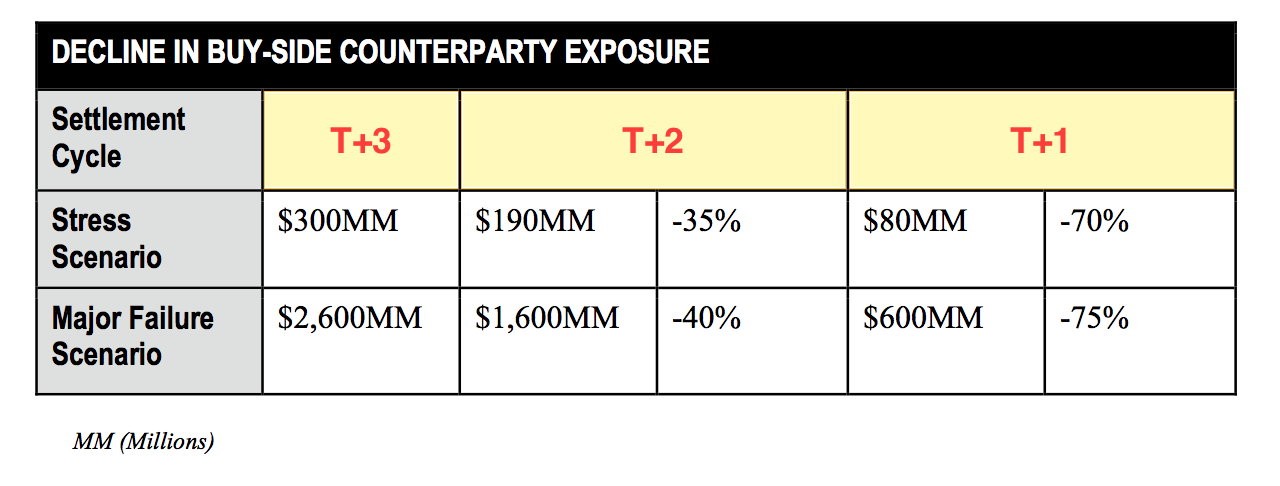
\includegraphics[width=1\textwidth]{exposure.png}
\caption{Impact of reducing settlement times on exposure}
\centering
\label{fig:exposure}
\end{figure}

Among the latest innovations we can count the apparition of the distributed ledger technology (DLT) - databases that are spread around the network and share information across multiple sites \cite{pwc}. The first of its kind was the blockchain conceptualised by Satoshi Nakamoto, which was the supporting infrastructure for Bitcoin (the famous digital cryptocurrency) and which became a popular alternative to common financial practices, allowing users to transact without the need for a third-party intermediary \cite{blockchain}. But can this be fully adopted in the financial world to replace traditional banking?
\subsection{Objectives}
\label{sec:Objectives}
With respect to the question above, the objective of the project is to find the best solution that can increase productivity (by decreasing trade processing times), lower costs (by relying less on the capabilities of a clearing house) and enhance the trading experience (by unleashing the full potential of trading), whether it is a DLT or an alternative. Although an ambitious goal, this project sets out to pave the way for replacing clearing houses with a distributed ledger solution that will bring clearing and settlement times from three days to a few seconds. 
\\ \\
This thesis will explore proposed solutions, including general blockchains (such as Bitcoin's blockchain \cite{SNakamoto:Bitcoin} and BigchainDB \cite{DBC}), financial blockchains (Ripple \cite{Ripple:docs} and BitShares \cite{BS:tech}) and blockchain-inspired financial solutions (Corda \cite{Corda:code}) and how they can be incorporated into current business practices. We will establish a set of requirements and investigate the applicability of each system by looking at their salient features and how they compare against the demands. It should be clear that we are not expecting any of these to be completely appropriate and that we start off by investigating which system is the closest to the ideal solution and what features can be sacrificed. It is a given that most of the requirements of this new system will be driven by the current features of traditional banking. However, it must be noted that some of these have to be adapted to satisfy the new infrastructure and frameworks used.
\\
After choosing the most appropriate system to work with, a series of supporting applications that will extend it will be implemented. These explore in more depth different salient features and how they differ from the current processes or other solutions. They will also attempt to test any claims made without formal proofs. Another goal of the project is to develop a demonstrative application that wraps all the useful behaviour researched in this report into a product that can be used by people without programming background. The aim of this is to show that the Internet of Finance \cite{CMM:RN} is an achievable concept. Finally, the thesis will look at some social implications such an implementation would have, particularly the challenges the system faces from a reputational and legal standpoint, as well as the consequences of making clearing houses redundant.
\subsection{Contributions}
\label{sec:Contributions}
From the programming point of view, the codebase used for the project is Corda - a distributed ledger platform built for the financial world. The decision for this choice is further discussed in Section \ref{sub:Corda}. The main contributions of the project are the following:
\begin{enumerate}
\item \textbf{The implementation of a new asset class representing shares.} We extended the functionality of the system by enabling agents to trade other types of assets besides cash and simple commercial papers. This included modifying the underlying structure of a bank's internal database to include records of share contracts. The share contract was designed taking into account three main capabilities - issuance, movement and transfer, which are discussed in more detail in Section \ref{sub:Contract}.
\item \textbf{Issuing shares from a mocked exchange.} Given the fact the system is mainly focused on the trading capabilities between banks, we had to populate each bank's ledger with cash and shares. While the cash issuer was already implemented, we needed a solution to issue share contracts under strict permissioning rules (avoiding self issuance, for example). This was resolved by the introduction of an ``exchange" entity which is detailed in Sections \ref{sub:Nodes} and \ref{sub:cashissuers}.
\item \textbf{Trading shares between two parties.} The main success of the project is achieving a correct trading cycle. Shares are being exchanged in return for cash, with the respective contracts being recorded in each individual ledger. Transactions are verified two-fold, both from the point of view of internal correctness (the right amount of cash, the right shares) and external correctness (forbidding double spending). More details on the trading facilities are provided in Sections \ref{sub:Contract} and \ref{sub:TheFlows}.
\item \textbf{A distributed system (over several machines) providing a web interface for issuing and trading shares.} This showcases a real-world example of what the system could look like and the ease with which trades would be recorded in the ledgers. An explanation of the important actors of this system and how it works is provided in Section \ref{sub:sharedEX}.
\item \textbf{A distributed system representing a random marketplace which emulates real-world trading circumstances.} This demonstrates the system can be used in a real-life context where there are many trades happening at the same time, between many different parties. It proves that clearing and settlement is almost instantaneous as well as the scalability of the system. More details can be found in Section \ref{sub:mkt}, detailing this application.
\item \textbf{On-the-fly addition of participants to the banking consortium.} This enables new participants to be included in the network (upon careful examination and permissioning, as well as the completion of Know-Your-Customer practices). The addition is proved to be done on-the-fly, i.e. without the need for a global restart of the network, in Section \ref{sub:flynode}.
\item \textbf{System analysis and implications.} An evaluation will be provided on the performance and security benefits of the system, as well as a discussion on the implications of making clearing houses obsolete in Section \ref{sec:Evaluation}. Moreover, we will look at any challenges the industry will experience when faced with a technological overhaul (like the one proposed in this project) in Section \ref{sub:challenges}.
\item \textbf{Some infrastructure enabling auditing.} This proves that auditing by external agents can be done easily and according to current regulations. The provided infrastructure shows that a regulator is able to access historical trading information for particular transactions. The current requirements for this step and other details are explained in Section \ref{sub:reg}.
\end{enumerate}
\newpage
\section{Background}
\label{sec:Background}
Traditional banking has lost its appeal in this digital era. Fast payments, done via your mobile phone are the norm now. The push for the industry to focus on the individual has been able to transform the customer side of the business. However, the infrastructure for corporate banking follows the same monolithic pattern as 40 years ago and digital developments have been slow throughout \cite{slow}. Although there have been attempts to modify this and modularise everything, perhaps the best solution is to start with a clean slate. Why is this so important now? As mentioned before, latencies and human errors are the main drivers of this move to update the systems. But perhaps we should also be looking at the cost of the current applications as opposed to a simpler, modern protocol. Industry experts estimate that \$15bn-\$20bn could be saved in costs by adopting a distributed ledger technology by 2022. These costs mainly come from the fees for cross-border payments, securities trading and regulatory compliance \cite{Clearing:cost}.
\\ \\
However, a ``deadline" of 5 years for implementing a completely new base-layer system seems daunting. A more reasonable alternative is to pin-point exactly the areas that introduce the most problems, whether they are related to risk or costs, and develop a solution to replace those. This would open the financial world to more opportunities that can be built on top of this solution and it would increase the modularity of technological systems. To be able to determine which part of traditional banking is most in need of change, we need to take a look at the current state of the overall process that drives banking. 

\subsection{Traditional Banking}
\label{sub:TraditionalBanking}
The banking ecosystem is very complex and the idea of managing a complete, industry-wide change is perhaps an unachievable goal at this point. This project focuses on a subsection of this ecosystem, more specifically \textbf{the optimisation of post-trade processes in stock trading: clearing, and settlement}. This section will look at some important concepts used throughout the project, such as financial instruments, the life cycle of a trade and the role of clearing houses in it, and applicable regulation.

\subsubsection{Financial Instruments}
\label{sub:FinancialInstruments}
Financial instruments are tradeable assets such as cash, ownership or a contract that gives the right to deliver or receive another financial instrument \cite{FA}. For example, securities are financial instruments and their issuer is the company that issues it. They can be stocks (ownership positions in a publicly traded company), bonds (debt investments at a certain interest rate) or options (the right, but not obligation to ownership) \cite{Security}. In contrast with options, futures are financial contracts that obligate the buyer to purchase an asset at a later date. All of them are traded differently and have different standards. 
\\ \\
There are 2 important dates for any securities trade: the transaction time and the settlement time. The former is related to the moment when the transaction occurs, while the latter represents the day in which ownership is transferred. This is further discussed in Section \ref{sub:LCOAT}. However, to give an example of a downside of the current banking system, securities have various settlement periods. Currently, the standard settlement time for a stock trade is 3 days, with some countries implementing a 2-day period. That means that if a person buys a stock on Monday, that transaction will be settled on Thursday \cite{TTimes}. This is important to know because it determines when exactly the client owns the stock or receives the money and can influence what actions he can perform from his account. A discussion about the legal restrictions due to this late settlement time is detailed in Section \ref{sub:Regulations}.
\subsubsection{Life Cycle of a Trade}
\label{sub:LCOAT}
This section aims to present a high-level view of the steps a trade goes through, from the decision to initiate a trade to the final settlement part. For the examples given, we will be focusing on an order to buy some shares in the stock market. The five main parts of a trade are as follows \cite{TradeCycle}:

\begin{figure}[H]
\centering
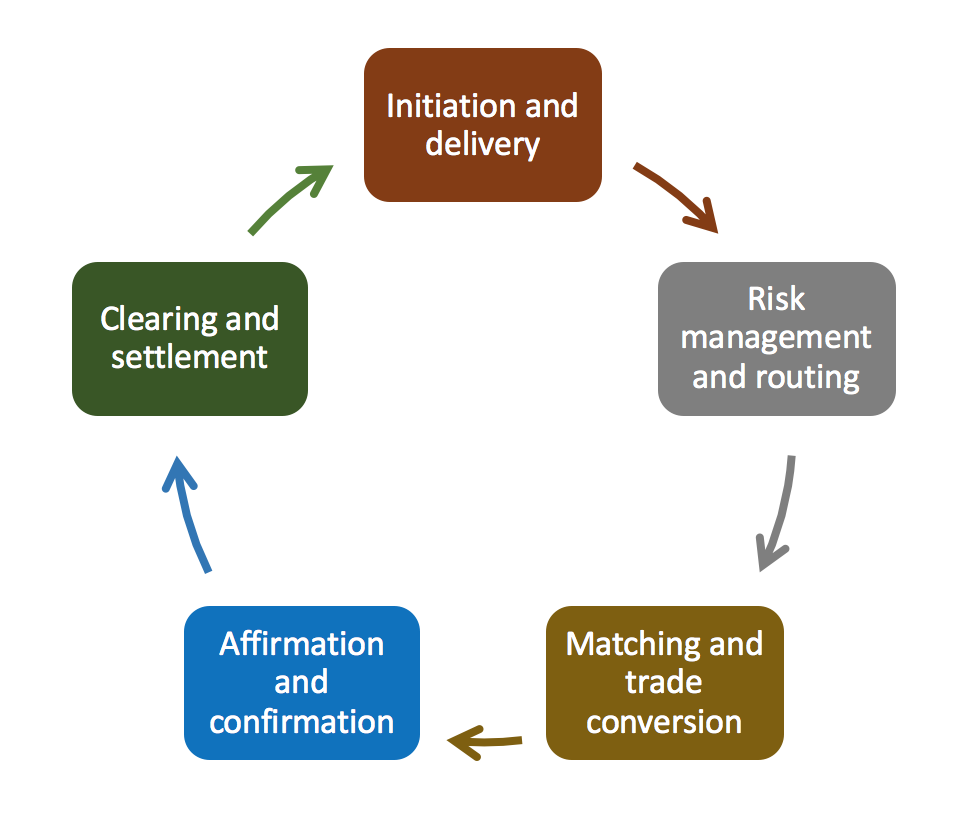
\includegraphics[width=0.9\textwidth]{lcoat.png}
\centering
\caption{The life cycle of a trade}
\label{fig:scheme}
\end{figure}

In the \textbf{initiation and delivery} stage, the client places the order to the broker. This can be done via any existent communication channel (phone, fax, online trading). It is now the broker's responsibility to register all the details of the order correctly and accurately so that no errors appear during the processing stage. Next up, in the \textbf{risk management and routing} step, the broker has to perform critical checks to ensure the client is a reliable source. Moreover, to control the risk, the broker also has to check whether the client has enough margin money (i.e. a sufficient balance to perform the trade - calculated based on the level of exposure and risk that the broker would be facing) or enough stocks (depending on the order type - buy or sell) to place the order. After the suite of checks finishes successfully, the broker gets a confirmation about the order and its execution begins or is delayed according to the terms defined by the two parties. 
\\ \\
The \textbf{matching and conversion} part follows. All such orders are collated and sent to the exchange, which allots the best price available to investors. Once the order is executed, it is converted into a trade and the broker receives a confirmation message that he has to pass over to the client. For the fourth step, \textbf{affirmation and confirmation}, there is a custodian agency that assists institutions in the clearing and settlement activities. They receive all information existent about trades and review their terms. If differences are found between the desired order and the actual trade (security mismatch, incorrect order type, different charges than the ones agreed upon), the custodian rejects it; otherwise, the broker receives confirmation. 
\\ \\
The last step encompassed a plethora of operations, which is why the delay introduced by Clearing Houses is often very high. \textbf{Clearing} refers to the net obligation at the end of a trading period (say, a day). To better understand this, we can take the following example. Alice buys 100 shares in Company A, for \pounds 100. She then sells 10 shares in Company A (for \pounds 10) and then she sells 10 more. Each of these actions are considered an individual transaction, but overall, in the clearing stage done at the end of the day, she reports that she has 80 shares in Company A and spent \pounds 80 (\pounds 100 initially, then received \pounds 10 twice from the shares sold). Now, in the \textbf{settlement} part of the trade, the shares and money have to transfer ownership. Therefore, what essentially happens is that \pounds 80 go out of Alice's account and 80 shares are credited to her account, since the individual transactions are bundled together. At this point, the trades she performed are considered complete \cite{TradeCycle2}. It is important to underline that the reason why it takes so long for the clearing stage to be completed is because we have to wait until the end of the trading day to group all trades together. A graphical description of Alice's trades is shown in Figure \ref{fig:alice}.
\begin{figure}[H]
\centering
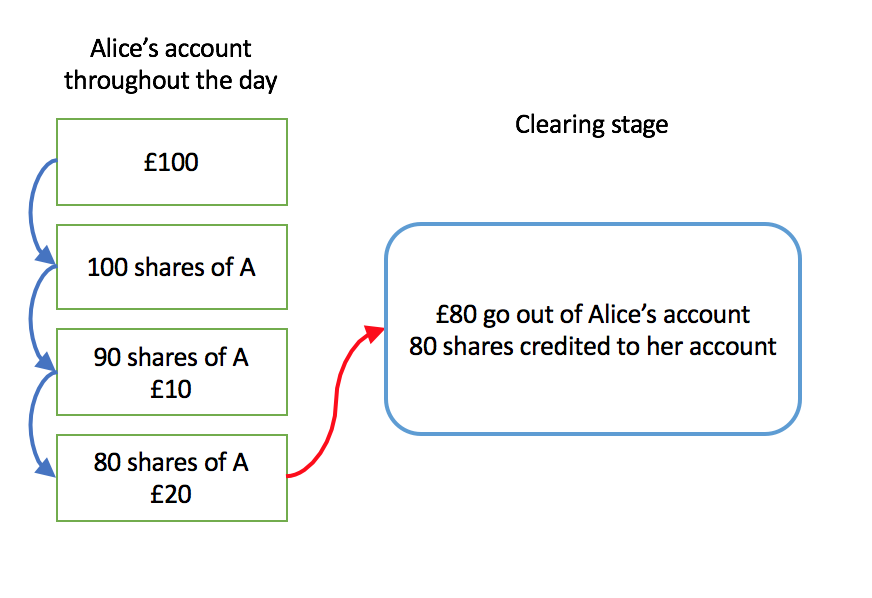
\includegraphics[width=0.7\textwidth]{alice.png}
\centering
\caption{Alice's daily trades}
\label{fig:alice}
\end{figure}

\subsubsection{Clearing Houses}
\label{sub:CH}
Given that clearing houses are the most important topic discussed in the project, we will go in more depth about their responsibilities and capabilities in this section. The main aim of a clearing house is to reduce the risk introduced by the delay in trade settlement. Instead of Alice trading directly with Bob and Carol with Dan, they each trade with a central counterparty (CCP). Once the details of the transaction are decided, the contract between Alice and Bob is basically split into two subcontracts - Alice with the CCP and Bob with the CCP. Since everyone interacts with the CCP, the clearing house is able to match orders at the end of the day at the best price. Now, the clearing house is also responsible to all members for the fulfilment of contracts \cite{clearinghouse}, becoming a legal counterparty to each trading party \cite{whatclearing} \cite{whatclearing2}. This means that the clearing house guarantees the trade will take place, even if one of the parties involved defaults before it satisfies its obligations. \textit{Market risk} is eliminated this way - the remaining party is not exposed to the price changes that occurred after the first trade was initiated since it does not have to perform the trade again. Once the assets' ownerships have been exchanged between the two parties, the delivery versus payment process is complete.
\\ \\
Since every transaction is processed within the same institution, clearing houses offer the possibility of efficient reporting. They are advantageous because they also provide more rigorous risk management methodologies than market users. This has the downside that participants have to contribute high amounts of collateral to be able to use the CCP, making it an expensive alternative. According to a study for SWIFT, the estimated costs are of \$5-10bn for clearing activities, \$40-45bn for the settlement, custody and collateral management and \$20-25bn for post-trade data and analysis \cite{DLTclearing}. 

\subsubsection{Risks and Bottlenecks}
\label{sub:Risks}
It is clear that the main bottleneck appears in the last step of the trade's life cycle. Usually the wait to have your account credited goes over 2 days. Not only is this an inconvenience for customers, but it is also an element of high risk. The Clearing Houses, which deal with the entire clearing and settlement process are subjected to default risk from any of the clearing members. If a clearing member defaults, the Clearing House is still under obligation to fulfill its duty for the other party in the trade. These costs are varied and depend on the type of financial instrument traded (futures or options) \cite{CHRisk}. Operational risk can also occur through system failure, human errors or inadequate management. Obviously, the usage of another entity in the trading cycle has many implications - most of them negative, from a productivity point of view.
\\ \\
Since latency and risk are heightened by the presence of Clearing Houses, their role should either be completely replaced or their duties shrunk so that they have less responsibility. This sounds like an ideal situation that is hard to reach by using the current infrastructure. There is not a way to record transactions in a short period of time, avoiding the detour via the Clearing House. However, the possible replacement of the deprecated infrastructure discussed above could facilitate development and getting to ``immediate" clearing and settlement of trades. (To be noted that ``immediate" will become one of the requirements for the system that will be presented in this thesis. However, this term is relative to the current process and can last as long as 15 minutes. An upper bound will be put on this, depending on further research done in subsequent sections.) \\
\begin{figure}[!htb]
    \centering
    \begin{subfigure}[b]{0.48\textwidth}
    	\centering
        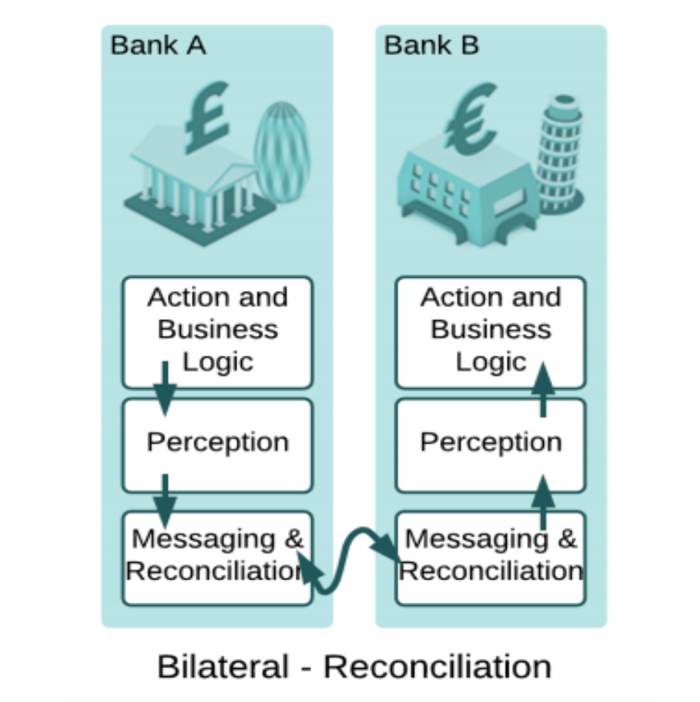
\includegraphics[width=1\textwidth]{bilateral-rec.png}
        \caption{Bilateral reconciliation of records, matching transaction details after each party applies its own business logic}
        \label{fig:bilateral}
    \end{subfigure}
    ~
    \begin{subfigure}[b]{0.48\textwidth}
    	\centering
        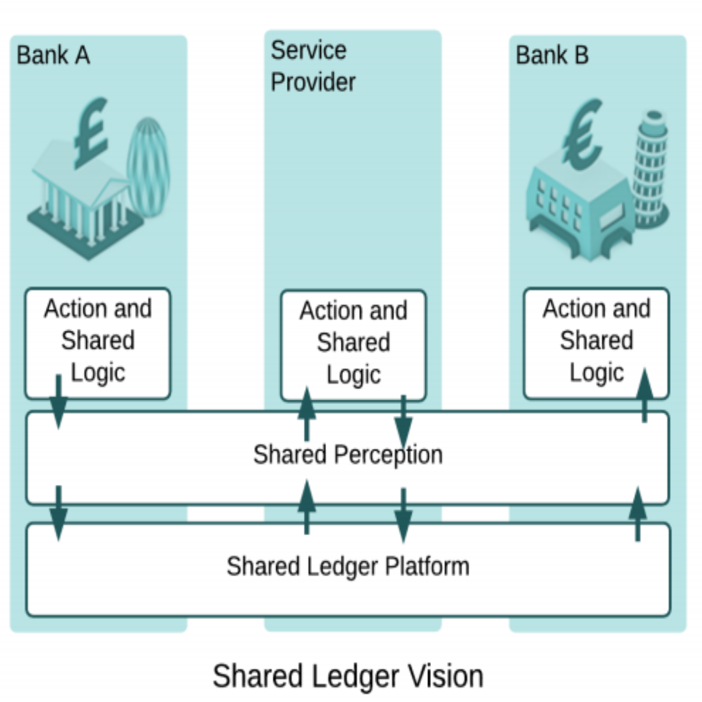
\includegraphics[width=1\textwidth]{shared-ledger.png}
        \caption{Schematic representation of the shared ledger implementation (along with the the technology service provider)}
        \label{fig:shared}
    \end{subfigure}
    \caption{Ledger implementations: traditional vs. ideal solution \cite{Corda:IP}}
    \label{fig:reconciliation}
\end{figure}

In traditional banking systems, it is common for every bank to have its own view of the ledger. This is not the only piece that differs between banks, the business logic implemented having various discrepancies too. To be able to reconcile records, a messaging system has to be in place. This adds another layer of complexity and potential sources of risk and errors - reconciliations might fail for several reasons (record mismatch, human errors when transferring data over the network). This can be visualised in Figure \ref{fig:bilateral}. However, in the ideal system Alice and Bob are using, this is no longer a problem because of standardisation of protocols and the shared view of the world. A technology service provider would support the common business logic between banks and manage the perception of the data to ensure integrity. This implies that market infrastructure providers would have to come up with competitive ideas instead, shifting the paradigm. This ideology is presented in Figure \ref{fig:shared}.

\subsubsection{Regulations}
\label{sub:Regulations}
%%% bring up mifid pls
Since stocks are traded on an exchange, a clearing requirement has been in place to manage risks for a long time \cite{etdclearing}. With the introduction of the European Market Infrastructure Regulation (EMIR), the clearing obligation appeared for over-the-counter derivatives, too \cite{emir}. While this project only looks at stock trading, its findings will be useful in the push for implementing a similar system for OTC derivatives.
\\ \\
However, one piece of regulation that directly affects stock trading is \textbf{Regulation T}, which has been in effect for cash accounts since 1934 \cite{settledate2}. As mentioned before, the settlement date for stocks is three days after the trade is executed. By this date, the buyer has to pay for the shares that have been delivered by the seller and a failure to comply with this rule leads to freeriding. According to the Federal Reserve Board, a 90-day ban should be put in place for any violating account. There are two ways of freeriding. The first is when a buyer's deposit bounced, but the stock purchased with that deposit was sold to cover the negative balance. The second is when the proceeds from one stock sale are used to purchase new shares, but these new shares are sold before the first sale is settled. To note here that a person can actually buy more shares legally, \textbf{but only if they have the required amount in settled cash} \cite{settledate}. This is obviously an obstacle for traders as it prevents a fluid manner of trading.
\\
\begin{figure}[!htb]
    \centering
    \begin{subfigure}[b]{0.8\textwidth}
    	\centering
        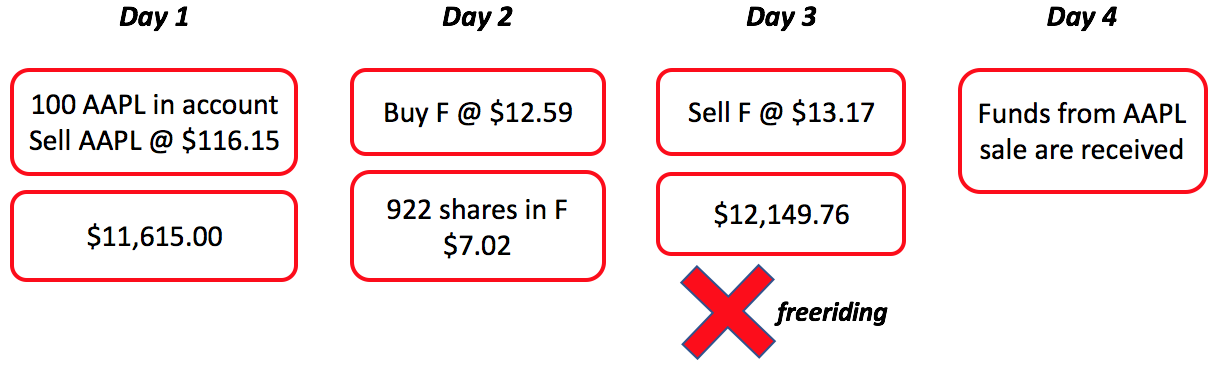
\includegraphics[width=1\textwidth]{freeriding.png}
        \caption{Temporal representation of freeriding}
        \label{fig:fr1}
    \end{subfigure}
    ~
    \begin{subfigure}[b]{0.8\textwidth}
    	\centering
        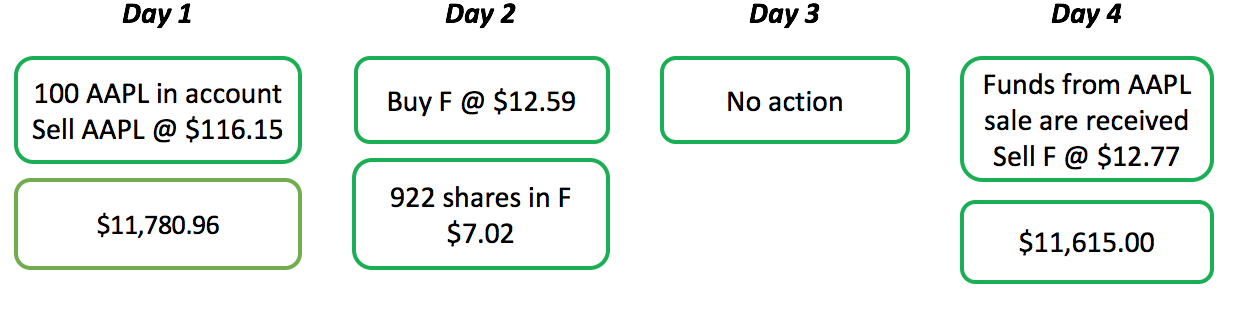
\includegraphics[width=1\textwidth]{nofreeriding.png}
        \caption{Temporal representation of correct trading}
        \label{fig:fr2}
    \end{subfigure}
    \caption{Freeriding}
    \label{fig:freeriding}
\end{figure}
\\
To better understand when someone can sell a security in their account, let's take the following example detailed in Figure \ref{fig:freeriding}, based on data for Apple Inc. (AAPL) and Ford Motor Company (F) between the 30th of December 2016 and 5th of January 2017 \cite{yahoo}. Suppose we are starting just by having 100 shares in AAPL in our account. On the first day of this trading example, we sell the shares at \$116.15. The funds now appear as ``unsettled funds" in our account and we do not have additional cash previously deposited. On the second day, we decide that Ford is a good stock to buy. We can now purchase F with the sale proceeds from the previous day (even though they have not been settled) - we have enough for 922 shares since F trades at \$12.59. At this point, we have in our account 922 shares in F and \$7.02. Next day, suppose that an important event causes some volatility in the market and the share price of F rises sharply by 4.6\% to \$13.17 a share. We want to sell our shares in Ford since that would provide a profit of \$534.74. But this would mean we are freeriding - the funds from the initial AAPL sale have still not settled so essentially, we would be selling some shares that we did not own with our own cash. The correct procedure, would be to wait until the fourth day, when the funds are settled and only at that point sell the shares previously bought. However, this means that we'd sell at \$12.77 - offering a profit of barely \$165.96. Of course, there are ways to avoid this - instead of having bought F with the sale proceeds from the AAPL stock, we could have done that with additional funds from our account that had been settled before we had done the trades.
\\ \\
It is clear that by shortening the settlement cycle, Regulation T would become obsolete or have a much smaller applicability for normal cash accounts. If trades were settled immediately, the funds we were in possession of could be used at any point after the previous trade, for any trading activity. However, high frequency trading (HFT) firms already bypass this regulation. Effectively, this can be done through multiple ways, such as by having a margin account. The difference is that you have an amount of collateral which should be large enough to cover any potential losses. Therefore, this allows frequent trading without having to wait for settlement, even if you are selling some recently purchased shares (with unsettled cash). However, this is not very useful for some investors, because a margin account might require around \$25,000 in collateral to be able to perform these frequent trades \cite{marginACCT}. Another reason why Regulation T does not apply for HFT firms is because they usually transact different financial derivatives than the ordinary stocks mentioned up until now. Therefore, by trading derivatives such as futures or options, they are able to enter into and exit out of the given positions in a matter of split seconds \cite{marginEXP}. 
\\
HFT firms are starting to get more and more regulated, just as traditional banking, with the introduction of the new \textit{Markets in Financial Instruments Directive} (MiFID II) building an extra layer of security on top of the existing guidelines \cite{mifid2}. Its implementation will have an impact on the trading that is analysed in this project as well. The most important change MiFID brings is the obligation for \textbf{transparency} \cite{transparency} - trades have to be published as soon as they become available, exchanges have to provide full reporting of their business and only pre-approved venues should be used for derivatives trading \cite{mifid2off}.

\subsection{Requirements}
\label{sub:Requirements}
By this point, we have highlighted the need to reduce settlement time for trades and explained some of the benefits this change would bring. The most natural course of action at this moment is to attempt the introduction of a blockchain-like system in the financial world, given that it satisfies all the needs the industry has outlined. For this, there have been many financial institutions and advisors releasing recommendations about the requirements such a system should accomplish. The UK Government Chief Scientific Adviser discusses several characteristics that a blockchain should have for banks to use it \cite{GOVReq}. The European Securities and Markets Authority started a discussion on the usefulness of distributed ledger technologies and released guidelines that companies should follow when implementing these technologies \cite{ESMA}. This project takes some of these recommendations as high-level requirements, but we will go in more depth to explain what they actually entail (for example, what does `high performance' actually mean?). 
\\ \\
\textit{High performance and low latency:} There has been a theoretical proposal for a speed of at least 100,000 transactions per second for any new system \cite{Chinese}. This makes sense in today's context and the rapid developments we are facing. As a comparison, VISA has a peak of 56K TPS \cite{visa}, but only handles on average 2K TPS every day \cite{Scalability}. However, the decision takes into account an increase in trading activity. To be able to assess this in the chosen systems, we also have to take into account latency introduced by other factors (extra nodes in the network, for example) or the bandwidth used. 
\\ \\
\textit{Efficiency and costs:} Institutions have to take into account the cost of implementing the new systems, but also miscellaneous costs such as onboarding. This depends on the learning curve of the introduced system. Therefore, the requirement is to build a system that is intuitive, easy to use. An analysis should be done on the difference between current costs of maintaining antiquated systems and the expected costs for the new system. Integration costs and efforts should be factored into this section, too.
\\ \\
\textit{Security and privacy:} The most important characteristic for the financial industry is related to security. There are plenty of ways that information can be leaked and we need to make sure that any vulnerability has been taken care of in a potentially implementable system. Some characteristics that fit this category are: being able to hide transaction information, obfuscating the IPs of the participants, avoiding the identification of participants from the keys the use and retrieving their trading patterns, dispute resolution and the correction of mistakes and the general avoidance of information leakage. 
\\ \\
\textit{Permissioning and memberships:} Related to the previous point, the permissioning system would enhance the privacy of the system. Therefore, we should be talking, at least in the initial form, about a consortium of banks. They would be governed by a superior, objective, trustworthy entity. Any new members would be able to join the consortium after passing important checks related to system requirements and internal security protocols.
\\ \\
\textit{Compliance:} The current banking system has in place several monitoring mechanisms to prevent illegal trading. Among these we can count Know-Your-Customer, Anti-Money Laundering and Anti-Terrorist Funding controls. Some banks are not allowed to trade with certain high-risk countries. All these have to be included in the design of a digital platform that seeks to reinvent the banking world. Moreover, there should be the possibility of having auditors (or audit nodes, as an example) that can monitor every transaction. They can perform checks to ensure the financial reporting is reliable and compliant to applicable laws and regulations \cite{GS:Audit}. The auditing facilities can either be internal (for the company's own monitoring) or external (having a general view of the trading world and the transactions performed). To aid in this process, the system should have timestamping abilities, which are important for determining transaction times, durations and different events. Being a live, real-time system, it is hard to ensure that all clocks are maintained synchronised, so these timestamping facilities should allow for time ranges instead of fixed time points. 
\\ \\
\textit{Reliability and persistence:} Clearing Houses are SIPS (Systemically Important Payment Systems). Countries either have a Real-Time Gross Settlement system or there are systems serving multiple countries (the pan-European TARGET2, for example). Their two key elements are the transfer of information between the payer and the payee banks and the settlement, which is considered irrevocable and unconditional \cite{RTGS}. Their criticality means they have to be extremely reliable. As an example, TARGET2 deals with the settlement of around 350.000 transactions daily \cite{TARGET2}, and it is only dealing with the Eurozone. Obviously, this means that replacing such a system will be a big task and the onboarding time will be proportional. A thorough analysis into the reliability of the new system will have to be performed to ensure it is up to the standards banks are looking to achieve.
\\ \\
\textit{Scalability:} The new system will have to be able to incorporate several nodes (the banks). They will represent the consortium that will be able to use the system seamlessly. However, there have to be alternative options for the banks that are not using it. The integration between the two options is of utmost importance to be able to make a smooth transition for the banks who choose to be part of the consortium and to be able to continue normal trading procedures as before. Performance is the characteristic that we have to look at here - will it be affected by the extension of the consortium? A good approach would be to start with a small consortium of banks and gradually extend the network as the system's reputation grows.
\\ \\
\textit{Network types:} The consortium of banks that will operate on the system will have to be linked by a very high-speed network. The way the system will actually be implemented gives more freedom of choice - peer-to-peer, private peer-to-peer or even friend-to-friend (where nodes have direct connections only to other nodes they know). There has to be a guarantee that transactions can happen between nodes situated in different machines or regions. A study into local banks' networks in Italy \cite{Italy:networks} outlines the need for links between banks to further economic performance. Therefore, the network should support connections between nodes that are not directly connected too, to improve productivity. Also, the speed of the connections is important in trading, but does not present a significant importance in the clearing and settlement of trades. 
\\ \\
\textit{Currencies:} Cryptocurrencies have enjoyed public acclaim since the appearance of Bitcoin. However, there are plenty of downsides to them as well. Cryptocurrencies would be traded just like any other currency, meaning that they will have a certain value. This can turn out to be a negative side effect since for some cryptocurrencies their volatility is still too high. Of course, for a system that used blockchain (or a version of it), the usage of cryptocurrencies would be obligatory or recommended. But is this the only option to represent money? Financial constructs could be represented by using a version of fiat money tokens and securities tokens. Fungible assets (mutually interchangeable) can be represented digitally by adopting a certain state the client is in (for example, the state in which he \textit{owns} a certain \textit{fungible asset}). For fiat money, this holds regardless (i.e. a \pounds 5 note will always be worth \pounds 5). As an example, for bitcoin there might not always be the case of fair trade and markets might discriminate based on the bitcoin's ownership history \cite{BC:Fungibility}.
\\ \\
\textit{Consensus protocols:} There has to be a voting failure handling for the nodes participating in the system. Do we trust all the nodes? Maybe, but they can still be corrupted (during a possible attack, for example). Therefore, the consensus protocols or mining facilities that evaluate transactions have to be well researched. Moreover, there has to be an analysis into the processing type of these votes - are they done sequentially or in parallel; how many votes are required; what is the granularity level of the voting (per transaction or per ``blocks" of transactions?).
\\ \\
\textit{Wallets:} Every customer should be in possession of a container that has all the assets it owns. This digital container should have the mixed assets of the client. These assets have to be issued previously by a governing authority (a Central Entity, say). 
\\ \\
\textit{Usability:} The new system must be as similar to the previous one in terms of user interface. That being said, banking systems are famous for maintaining the same UI since the beginning of their application, solely for the reason that ``it works". Of course, brokers got used to the looks so, although there will have to be a change to refresh the design and bring it to more modern days, it should be done in such a way to cause as little disruption as possible. The applications developed in this project will not attempt to fulfill this requirement since there should be a direct collaboration between the potential users and the developers. Hence, the thesis only looks at the functionality of the presented systems.
\\ \\
\textit{Reputation and marketing:} Adoption of new techniques and frameworks is controversial in the financial world. Has it been tested enough? Does it feature all the requirements we have? Has it been used before? What are the failure rates and how trustworthy is it? Again, not all of these questions will be answered in this report, since the system would have to be tested in the real world, at a very large scale, to provide a very high level of certainty. Reputation - the widespread belief that the solution is good and trusted - cannot be easily quantified, so the proposed system will have to have a strong marketing campaign, along with partnering banks which are able to support development. An idea to increase the reputation would be to implement testnets and have experiments done on them by each bank that is thinking about adopting the new system.

\subsection{Distributed Ledgers}
\label{sub:DistributedLedgers}
Many believe that cryptocurrencies (and more importantly, the infrastructure they use) have the potential to ``disrupt" the financial world. They also agree on the fact that the lack of liquidity and their volatility currently represent a major obstacle. However, there is no doubt that the underlying technology of Bitcoin will ``alter the financial landscape" \cite{CMM:RN}. Therefore, we will look at these distributed public ledgers, both the original one and altered versions. The most prevalent type of these is often referred to simply as blockchain.
\\ \\
The most common salient features of blockchains are transparency (everyone can see the transactions on the blockchain) and redundancy (every node has a copy of all the blocks). They often run on P2P networks, use digital currencies and are based on mining to verify the transactions. This presents us with a lot of issues, were we to implement our system on one of the ``common blockchains". We do not desire transparency, we would like individuals' identity to be protected and trades to be private, hidden. Otherwise, the market would easily be influenced from a simple analysis of trades that took place. Moreover, the redundancy in every node does not suit us - it is a problem of cost and scalability, although methods have been designed to prevent any issues that could arise. Mining as a method of verification is costly as well, since it is based on the Proof of Work (discussed below) and \textit{rewards} the nodes who contribute computation power. In a financial blockchain scenario, we would not have to worry about monetary compensation, since all the nodes are working \textit{fairly} towards the same goal. The peer-to-peer network might not be suitable for our purposes since its design principle of avoiding all regulations is in direct contradiction with one of the requirements described. The use of cryptocurrencies serves the purpose of keeping the integrity of the original blockchain's principle. However, they can be replaced by digital references to cash liquidity or other assets. An in-depth discussion of cryptocurrencies and cash liquidity will be provided in Section \ref{sub:cashissuers}.
\\ \\
We showcased the need for creating a purpose-built blockchain-based solution, instead of adapting existing general ones. We will look in more depth into Bitcoin's original blockchain in a subsequent Section, \ref{sub:Insufficient}.
\\ \\
Two popular ways blockchains can verify transactions are mining (via Proof of Work) and Proof of Stake. While they both offer their own benefits, they have also been criticised, as will be explained below. However, we will be looking at other consensus algorithms that are more appropriate for this project, namely the BFT-SMaRt library (a variant of the Practical Byzantine Fault Tolerance algorithm) and RAFT (a \textbf{formally proven safe} alternative of Paxos).

\subsubsection{Proof of Work versus Proof of Stake}
\label{sub:powpos}
\textbf{Proof of Work} uses the power of computation to verify transactions. What this means is that nodes ``vote" the correct version of transaction history by contributing their resources in calculating very rare hashes \cite{PWPS}. Such a system needs to have 51\% of the total power to be validated, protecting against malicious users in this way. A hacker could attack the system by gathering more than half of the network hash rate - but the assumption is that this can never happen. Since there is a reward for contributing to the validation (the ``mining"), it is considered to be more profitable to use the computation power to verify transactions that to try to attack the system. However, there are some points that we should consider here. First of all, there is currently an upper bound on the number of bitcoins to be created and currently 76.9\% of all bitcoins have already been mined \cite{BC:UB}. This means that once the cap is reached, miners will no longer be rewarded in new bitcoins, but in transaction fees (possibly much less profitable). Another issue to look at in the case of Proof of Work is that nodes are ``devouring energy in the race for mining profit" \cite{PoW}. There should be an alternative that limits this energy consumption and is, in general, more eco-friendly. Moreover, the algorithm does not give a final decision, providing only a probabilistic approximation which does not fit the standards of the financial system \cite{Corda:TP}.
\\ \\
An alternative solution considered is \textbf{Proof of Stake} \cite{PWPS}. The concept is that instead of basing the votes on the limited \textit{computational} resources, they can be based on the limited \textit{coins}. Therefore, the ticket you are ``paying" to be able to vote is composed of the coins you own. Again, the same concepts apply - to be able to sign a transaction, you need 51\% of the existing coins. The benefits of this type of proof are related to saving energy (no computation power required) and attacks become more expensive, since we would have to buy 51\% of the coins (and the market would react by price appreciation, making the purchase expensive and effectively pointless). The limit is no longer defined by the total computational power, but by the total number of coins people have in their wallets. Unfortunately, this is not without fault either. One possible attack is related to double-spending, because Proof of Stake allows to mine different versions of the blockchain \textit{simultaneously}. Also, since the private keys for money already spent are ``useless", there might be people tempted to still accept money for them. An attacker can rewrite the history of the blockchain by mining with the old keys, at a specific point in the past. He is the one receiving all the rewards since he would technically own 100\% of the coins in his version of the blockchain. At some point, this alternative version of the blockchain will catch up with the real version and have a larger number of blocks. But nothing is preventing the network from switching to the malicious, manufactured blockchain, since technically it is the more recent one, with more transactions recorded. From this point onwards, the malicious user owns most of the coins in the network and can perform any attacks.
\\ \\
There have been developments in the implementation of both types of proof and their security has been improved (PeerCoin performs regular checkpoints preventing branching in Proof of Stake \cite{PWPS}). There have also appeared some hybrid combinations of the two such as Proof of Activity or Proof of Burn \cite{PAPB}. However, these are still theoretical approaches, so they cannot be used in industry systems. Ultimately, given the shortcomings of these algorithms, in this project we will be focusing on systems that provide a logically safe consensus protocol instead, such as RAFT.
\subsection{Available systems} 
\label{sub:AvailableSystems}
There are several industrial-grade projects that have taken off since the appearance of the first implementation of a distributed ledger. Some of them are general-purpose solutions, while others look specifically at blockchains for the financial industry. However, it is not the case that the distributed ledger has to be a blockchain. This section aims to look at whether the requirements established above are satisfied in each of the systems researched, and to what extent. 

\subsubsection{Some insufficient solutions}
\label{sub:Insufficient}
\textit{Bitcoin's blockchain:} This is by far the most popular blockchain and the market cap of its cryptocurrency was more than 17 times larger than the next most used one in February 2017 \cite{BC:MC}. But is it an appropriate base for applications able to revolutionise the financial world? Arguably, no. One of the biggest problems we would be facing by using this implementation is the performance. Currently, the peak number of transactions per second is 7 (not comparable to the 100K TPS we require for a system to be feasible for the financial industry). It is clear that unless drastic improvements are being executed, this BC does not fit our purpose. Even so, there are more hurdles that have to be overcome in order for this to become a possible solution. However, looking at the original implementation, it is a lot easier for us to compare the subsequent solutions. 
\\
The ledger offered by Bitcoin's blockchain is \textbf{public}. Everyone has access to the history of transactions and although they are cryptographically protected, there are possible identity leaks. For example, there can be an attack aimed at tracking spending habits for certain clients. The clients are identified by their keys, but nothing more is actually needed in this case - these patterns could influence the markets \textit{or} give an insight into what other people are trading, when and how. There are \textbf{no permissioning systems} in place, so anyone could participate in adding blocks to the blockchain (unless a membership subsystem is formed). Moreover, since this BC functions by employing Proof of Work as the verification method, there would have to be a consortium of dedicated miners able to support its activity. That means that there will be \textbf{extra costs} from providing computational power, as well as worries about the source of computational power (for example, would it be possible to use a botnet to mine?).
\\ \\
\textit{Hydrachain and BeihangChain:} Hydrachain is a private BC based on Ethereum and developed with the purpose of serving financial scenarios \cite{Chinese}. From the point of view of performance, it is an upgrade on Bitcoin's BC, but having 1K TPS is still not up to the standards desired. It has most of the same features of general blockchains, with some particularly interesting characteristics to note. Blocks are only created by ``leaders" (which would have to be defined as a superior entity in our financial system - potentially a Central Bank). Voting is done on each new block using Byzantine voting. 
\\ \\
Another private chain is BeihangChain, that performs \textbf{concurrent voting and data collection} \cite{Chinese}. This speeds up the process and reaches (at best) 24K TPS. Any node is able to create new blocks, but the voting in this BC is more sophisticated. Not only are new blocks being voted on, but also each transaction, increasing the number of messages being transferred between nodes.
\\ \\
These approaches are getting closer to our goal, but they have been developed to take care of individual scenarios at a time - a BC for trading and a BC for account information. Indeed, we are not seeking to build blockchains that completely support the banking system, but even so, these solutions are too restrictive. To use one of these 2 BCs for Clearing and Settlement is possible, but there are 2 main issues: the tests performed have been developed on controlled environments inadequate for our purposes and the source code is not available to the public (making it hard to extend and test it). Therefore, we will not be considering these mostly theoretical approaches further.
\\ \\
\textit{BigchainDB:} This approach claims to ``fill a gap in the decentralisation ecosystem" \cite{DBC}. It boasts amazing performance (1 million writes per second throughput) and low latency. Indeed, this is a scalable option and does fit most of our requirements: private, permissioned and performant! However, many have criticised its design for being fundamentally flawed. This is because all nodes are using the same RethinkDB cluster (a distributed database) which leads to extreme fragility. If, for example, one node becomes corrupted, it can simply execute a \textit{dropTable} on the cluster, leading the whole system to crash \cite{Sewer}. Obviously, we are not expecting any of the nodes in the consortium to be hijacked, since they are permissioned after a long series of checks. However, security can never be perfect and there will always be vulnerabilities and potential zero-days. The financial world cannot take this risk, therefore, from a security perspective, we consider this solution infeasible.
\begin{comment}
\begin{table}[]
\centering
\caption{My caption}
\label{my-label}
\resizebox{\textwidth}{!}{%
\begin{tabular}{@{}cccc@{}}
\toprule
\rowcolor[HTML]{C0C0C0} 
{\color[HTML]{333333} \textbf{Requirements}} & {\color[HTML]{333333} \textbf{Bitcoin}} & {\color[HTML]{333333} \textbf{\begin{tabular}[c]{@{}c@{}}Hydrachain and\\ BeihangChain\end{tabular}}} & {\color[HTML]{333333} \textbf{BigchainDB}} \\ \midrule
\textbf{Performance} & low (7 TPS) & medium (1K TPS) & high \\
\textbf{\begin{tabular}[c]{@{}c@{}}Security, privacy\\ and permissioning\end{tabular}} & \begin{tabular}[c]{@{}c@{}}transactions are\\ public, seen by all\end{tabular} & \begin{tabular}[c]{@{}c@{}}developed for \\ financial purposes\end{tabular} & some permissioning \\
\textbf{Compliance} & \begin{tabular}[c]{@{}c@{}}no protocols\\ implemented\end{tabular} & \begin{tabular}[c]{@{}c@{}}basic protocols \\ implemented\end{tabular} & \begin{tabular}[c]{@{}c@{}}no protocols\\ implemented\end{tabular} \\
\textbf{Reliability} & high & unknown & issues reported \\
\textbf{Costs} & \begin{tabular}[c]{@{}c@{}}mining and\\ transaction fees\end{tabular} & low & low \\ \bottomrule
\end{tabular}%
}
\end{table}
\label{tab:comp1}
\end{comment}
\subsubsection{BitShares and Stellar}
\label{sub:BSS}
\textit{BitShares} is a platform for financial smart contracts, developed specifically to address problems in traditional cryptocurrencies such as high volatility \cite{BS:TP}, discussed in Section \ref{sub:cashissuers}, too. The founders intended to provide tools for the creation of both market-pegged assets and user-issued assets. Their practical payment solution does not rely on creating a price-stable asset, which can be dangerous because of issuers that might go bankrupt. Instead, it uses their proprietary cryptocurrency (\textit{SmartCoins}, which has a value pegged to another asset like US dollars or gold) as collateral in contracts. 
\\ \\
The system has plenty of advantages, offering ``financial instruments for anyone to use, with low barriers to entry". As a system of verification, it uses a Delegated Proof of Stake, which is the most efficient consensus protocol available \cite{BS:DPOS}. Because of it, the performance is also different than the systems presented above - it is able to perform 100K TPS if the infrastructure is being accounted for (i.e. the system is able to reach the highest level only if the network connections and node structures are of a high standard) \cite{BS:tech}. It also incorporates compliance techniques such as KYC, which were presented in the requirement list. To appeal to the corporate world, it does enable dynamic account permissions which eliminates some of the risk of hacking compared to the public ledger. 
\\ \\
However, there are some downsides to this as well. Because the system introduces a new cryptocurrency, there is again concern for price manipulation and market influencing. This is taken care of by pricing the risk into the premium paid, but there have not been tests on whether this is able to cause serious trouble in a real trading environment. Moreover, every transaction will incur a fee. This makes sense from the point of view of the company, because it has to be self-sustaining. But in the financial context, the goal should be to have a system that is able to encompass all the current business features without additional costs (other than the ones for running the machines/servers). This would disadvantage companies with large trading volumes. Even though the fees for BitShares would be priced into the fees of the brokers for handling transactions, a further cost-benefit analysis would have to be carried out and compared with other solutions.
\\ \\
\textit{Stellar} is a similar concept to BitShares, with a similar performance in terms of transactions. It uses a different consensus protocol, the Stellar Consensus Protocol (also named the Federated Byzantine Agreement model) which adds flexible trust to the classic Proof of Stake \cite{Stellar:TP}. It operates with an inflationary currency (Lumens) which facilitates multi-currency transactions and hinders DDoS attacks (because every transaction has a fee). However, this BC is focused on managing micropayments and is specifically targeting individuals, encouraging an expansion of the banking systems to the underbanked \cite{Stellar:docs}. Although it would be possible to focus on the conversion of Stellar into a corporate-facing company, there are currently other alternatives that seemed more appealing.
\\ \\
As the table in Figure \ref{fig:comparison} shows, while each of the solutions presented until now has a good part, their worst features would negatively impact the system we are planning on building. Therefore, we will not be considering these as possible building blocks for this project.
\begin{figure}[H]
\centering
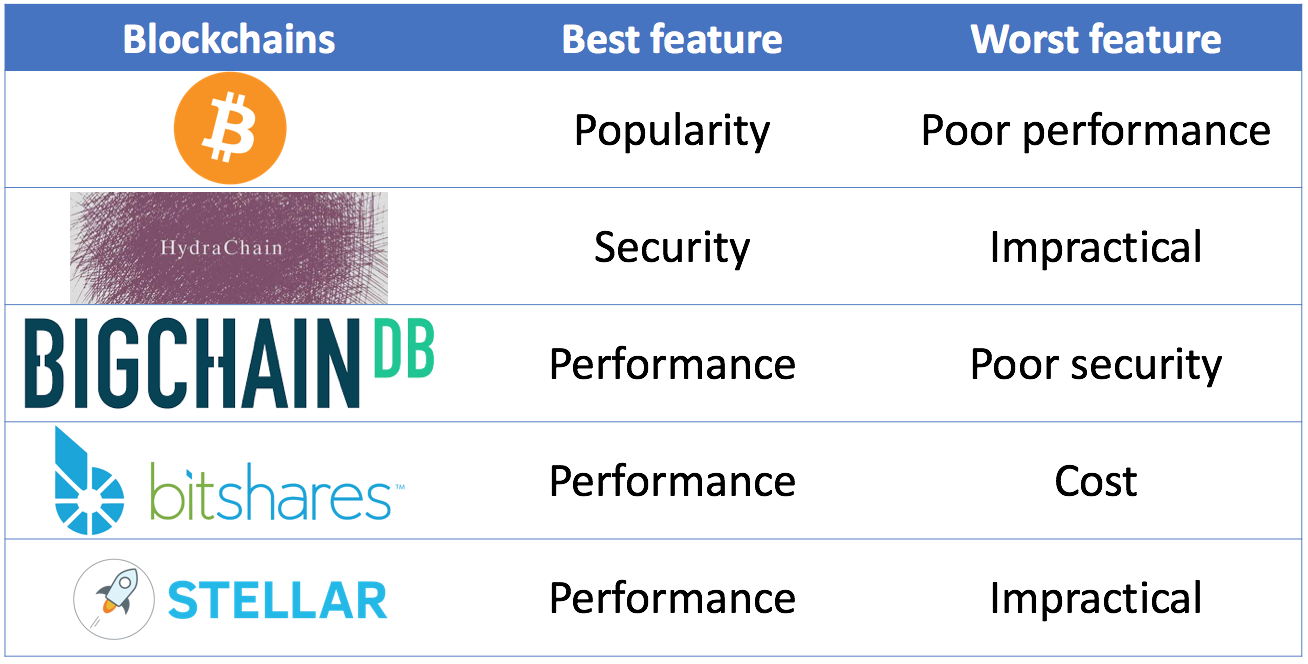
\includegraphics[width=1\textwidth]{comp.png}
\centering
\caption{Best and worst features of some blockchain solutions.}
\label{fig:comparison}
\end{figure}

\subsubsection{Ripple and Ethereum}
\label{sub:Ripple}
Ripple is one of the largest blockchain in terms of market capitalisation of its own cryptocurrency, after Bitcoin \cite{bitcoindominance}. Its distributed financial technology allows institutions to reduce delays when performing transactions and ensure their clearing \cite{Ripple:TP}. Through this on-demand payment, clearing risk is reduced and efficiency is improved. Moreover, the compliance processes related to tracking and investigation are aided by the infrastructure (the financial institution remains responsible for the onboarding process of clients). The diagram shows the structure of the Ripple system. To incorporate it in banks' systems, they have to be linked to a Ripple Connect node. The messaging (consisting of payment instructions, exchange fees, customer information and payment confirmations) is done directly between these nodes. For the settlement of the transactions, the nodes employ the Ripple Network (validators that perform cryptographical checks on the validity of the data) which also confirms the transaction to all parties involved.
\begin{figure}[H]
\centering
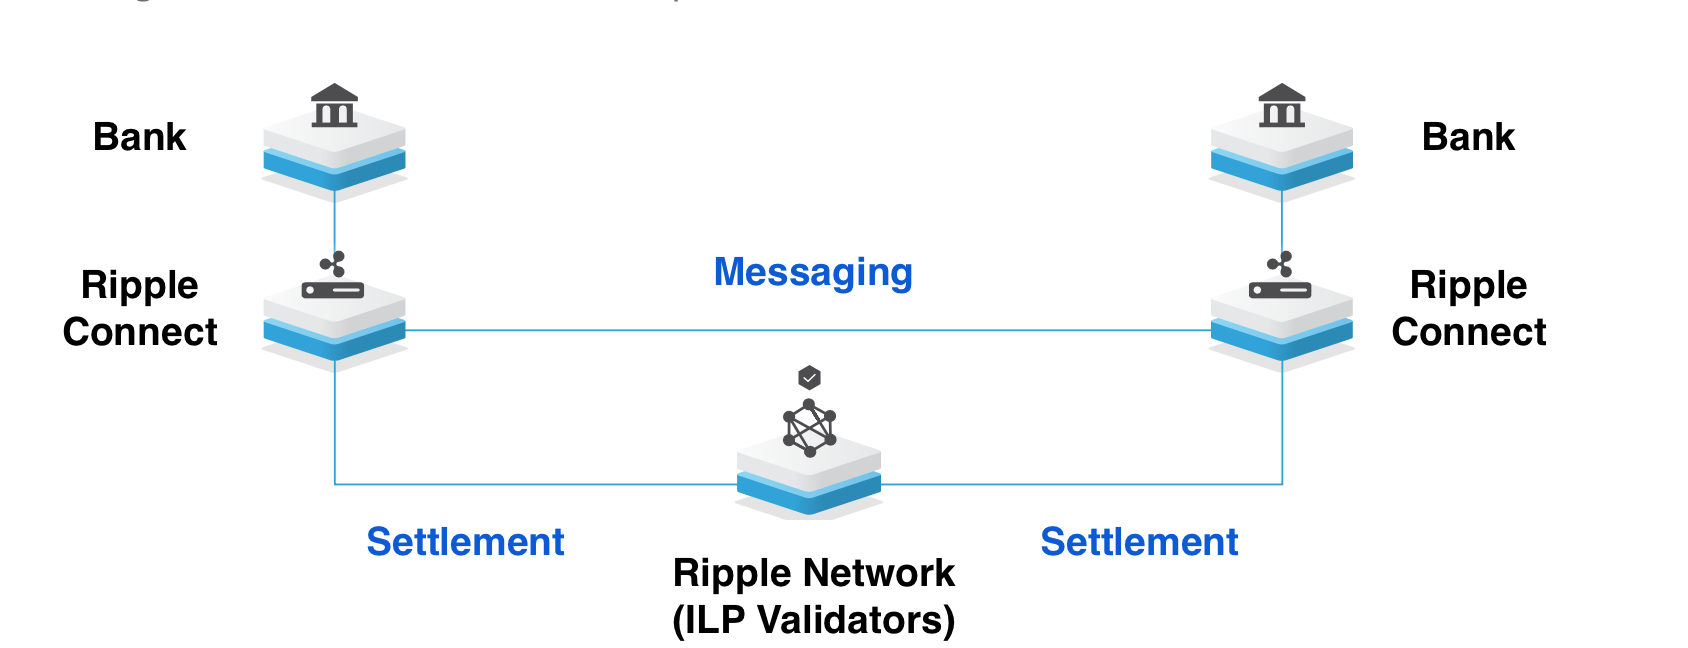
\includegraphics[width=1\textwidth]{ripple.png}
\caption{Ripple node overview \cite{Ripple:TP}}
\centering
\label{fig:Ripple}
\end{figure}

Ripple becomes a \textbf{technology service provider} in this case and banks are meant to have the Ripple Connect incorporated to be able to settle transactions over the network. The infrastructure is highly configurable and makes use of the Interledger Payment (ILP) validators (a byzantine-fault tolerant consensus algorithm) \cite{Ripple:ILP} \cite{Ripple:CP}. This protocol does not have access to the payment details, it cryptographically verifies whether the conditions for validity are met. 
\\ \\
The setup of the Ripple system is done by having a separate Ripple ILP Ledger which acts as a suspense account tracking the state of the funds. The process flow involves several API requests to Ripple Connect (getting the quotes, accepting them and locking them, for example). The actual payment process consists of 3 stages: sending the payment from the originating bank, executing the transfer over the Interledger Protocol and settling it, and receiving the payment at the beneficiary bank \cite{Ripple:TP}.
\\ \\
However, as it happens in Stellar, Ripple also uses its own cryptocurrency to stave off attacks by demanding a fractional amount for every payment. There are other concerns or criticisms against Ripple as well. In a review done by Jo Lang \cite{JoLang} there were issues raised such as the possibility of a fork in case more than 20\% of the network nodes do not agree on the validation of a transaction. All that being said, considering the system has been already in place for a few years, it has been subjected to higher amounts of peer reviews and reports contributing to the overall enhancement of the Ripple solution.
\\ \\
Ethereum was considered as an alternative for a brief period at the beginning of this project. However, there was a controversial hard-fork that happened at the end of 2016 meant to tackle the denial-of-service-like attack on Ethereum \cite{ethblog}. Given the decision was made without having an input from the majority of the users of the system or those that possessed the cryptocurrency used and most people were strongly opposed to the fork \cite{ethoped}, some of the trust in the system was lost \cite{ethhf}. Therefore, it was not studied in more depth and put among the candidates for a base system for this project. 
\subsubsection{Corda}
\label{sub:Corda}
The blockchain paradigm has the potential to revolutionise many areas - health services, elections and transparency in supply chains. However, the public nature of the ledger is frowned upon (at least for now) in the financial world. The final system to be presented in this section is Corda - born from the desire to have a blockchain-based solution that specifically caters to the financial industry and that is developed in concordance with expert guidance from the domain. Corda's proposition is based off the blockchain ideas, but the execution tries to maintain global databases at the core of the processes. Therefore, it puts forward the idea of a ``distributed ledger made up of mutually distrusting nodes" which enables the recording of different transactions in a single global database \cite{Corda:IP}. The platform is also abiding by the financial institutions desires of having a \textbf{regulated environment}. Moreover, by using the shared ledger and having the same perceptions about the data existent (transaction details, records, etc), there is no risk in mismatching records and therefore, no need for reconciliation.
\\ \\
This section will give an abstract introduction to the Corda ecosystem, present which requirements it is able to fulfill, determine the challenges in using this system and explore potential ways to expand on the existing codebase. This section is based on the whitepaper detailing the end-goal of the system - as opposed to other solutions presented up to this point, Corda is still in development. After having been open-sourced at the end of 2016 \cite{cordaops}, its parent company secured the largest investment for distributed ledger technology ever \cite{cordainv}, making it an almost guaranteed future success. This gave us confidence to have Corda as the codebase for our system, especially considering the involvement of the community in its growth.
\\ \\
From a high-level perspective, the end-goal is to allow parties to record and manage agreements reliably, privately and authoritatively \cite{Corda:IP}. The global ledger will have a distributed physical appearance, but will act as one logical component. The records contained on the ledger should be legally binding and open for investigation from compliance and regulatory entities. From the point of view of privacy, access to data is intended to be granted only to those who need it (therefore, the system works on a need-to-know basis) - the parties who take part in a transaction and the regulator entities present in the system. Therefore, instead of broadcasting transactions like in the typical blockchain systems, Corda makes use of the concept of \textit{flows} - multi-step transaction building protocols. These manage the transaction structure and ensure that all the requirements for a smart contract are met. For example, we would use a flow to perform a transaction between Bank A and Bank B and broadcast the transaction only to the regulatory entities present in the system, besides the transaction participants.
\\
\begin{figure}[!htb]
\centering
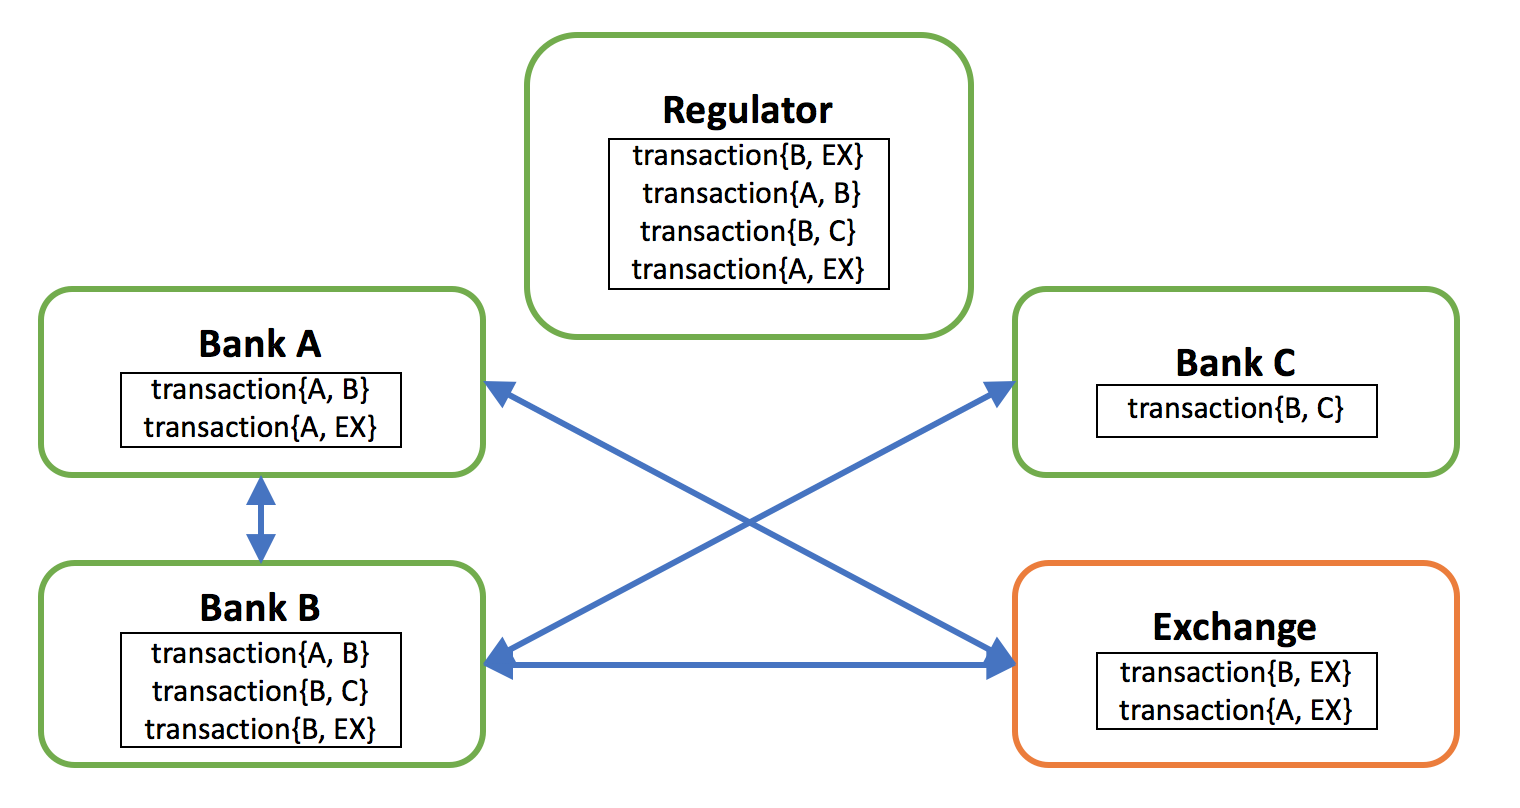
\includegraphics[width=1\textwidth]{broadcast.png}
\caption{Example of private transaction broadcasting and regulator surveillance}
\centering
\label{fig:broadcast}
\end{figure}
\\
Looking at Corda's most important aspects, we can observe how they satisfy the requirements we have previously set. Being specialised for use within regulated banking institutions and developed under the assumption of an adversarial security environment, protection of data and privacy have been critical in Corda's implementation. Data is shared on a \textbf{need-to-know basis}, therefore not everyone has access to all the records. This increases security because Bank C should not have access to a trade that took place between Bank A and Bank B. This can be observed in Figure \ref{fig:broadcast}. Corda does not employ a mining mechanism for the verification of data, nor a Proof-of-Stake approach. Instead, it uses the concept of ``pluggable services". The default should be the RAFT algorithm which is formally proven safe \cite{raft}, but this can be replaced by Byzantine fault tolerance systems. Moreover, the details of the transactions are kept private - using Merkle trees, they can be ``torn off" and only the root of the transaction will be validated cryptographically (the rest of the information is useless for the signing authorities and therefore hidden) \cite{Corda:TP}. 
\\ \\
Performance-wise, data is not completely replicated in each node, which adds another layer of efficiency and reduces delays introduced by the necessity of data duplication. Corda works with smart contracts that define the business logic of the ledger and enforce the validity of transactions. The JVM used in Corda is extended with a custom sandbox that restricts usage by enforcing security requirements and deterministic execution \cite{Corda:IP}. However, there have not been any tests regarding the number of transactions per second or the load a node can resist until now. These are planned to be performed or researched as part of this project, providing both quantitative and qualitative results to support any claims made.
\\ \\
The ideal scenario would see a consortium of banks running Corda, after specific permissioning requests from each institution have been analysed and granted. The permissioning service would sign off the requests and add the new party to the semi-private network. One important requirement would be for all of them to contribute to the network in an equal manner (i.e. they provide nodes that run on servers that match the hardware requirements). This way, the standards of the consortium will be kept high for everyone to benefit from the Corda integration. There will have to be a cost analysis that takes into account the integration of the new system, onboarding the brokers on it and maintenance needs. However, instead of directly replacing all the current systems with Corda, the founders seek a phased approach. This is supported by the platform's gradual integration of new nodes or its ability of combining networks based on applicability potential. This links well with the usability criterion, through which we want to ensure that both the engineers who have the job to integrate this system into the current banking processes and the users are going to be happy about the changes.
\\ \\
To be able to replace the Clearing Houses, Corda needs to prove it is reliable and persistent when dealing with transactions and contracts. Nodes are backed by a relational database which can be joined with data from the ledger, on request. Wallets (called \textit{vaults} in Corda) have the different assets that customers own and can also be accessed through SQL queries.  There will be further analysis into how the reliability is provided with Corda, as well as looking into data storage in Section \ref{sub:Performance}.
\\ \\
From the business logic perspective, transactions follow the Bitcoin structure, having inputs, outputs and signatures. The ledger records the ownership of assets through states. Corda does not use a cryptocurrency to represent other assets, especially cash. Therefore, the issue that may arise in this case is related to national fiat currencies which might not be fungible in some cases (because unless the issuer is a Central Bank, it could go bankrupt) \cite{Corda:TP}. We will be looking at asset representation and compare this with alternative solutions and cryptocurrencies in Section \ref{sub:cashissuers}.
\\ \\
Given that it has been less than six months since the code became open sourced, there are still a lot of unknowns with Corda. Many of its premises are not implemented yet, but the system in its current state was promising enough to constitute the basis for this project. It has to be noted that any tests performed on Corda code will not take into account possible optimisations that are expected to be done to the system after the implementation of all stated goals. The biggest challenge related to this project is the volatility of the codebase - development is in progress, therefore changes might occur at any point during the project. Along with these, there could be released similar applications or tests as the ones this project is attempting to present. Therefore, an active research will still take place even after the initial phase in which information about the system was gathered and any modifications and updates will be clearly signposted throughout the next sections. 
\\ \\
The potential ways to build on this system and present a prototype align well with the goals of the thesis. First of all, a suite of applications targeted at particular concepts present in Corda will be developed. These will test modularly the properties of Corda and how or if they satisfy the requirements. Besides the distributed ledger system, Corda also provides developers the option of building their own CorDapps, which are basically templates for different pieces of functionality one might require in a financial context. Therefore, the applications that will be created during this project might take the form of a CorDapp, if needed. These applications are mainly aimed at analysing the following:
\begin{enumerate}
\item \textit{Features}: asset class representation, asset issuance, trading facilities, system expansion, persistence
\item \textit{Security}: internal and external transaction validation, signing facilities
\item \textit{Compliance}: regulatory requirements, auditing facilities
\item \textit{Performance}: scaling possibilities, speed tests (transactions per second, for example)
\end{enumerate}
There will be a theoretical discussion looking at performance metrics, supported by practical examples. Finally, the end-goal of the project is to present a demonstrative application that will encompass some of the major features Corda has to offer. This could take the form of a CorDapp, with a user interface that blends in with the existing ones used in Corda. We want to showcase the main points we are analysing and, if the result is a positive one, prove that Corda can change the banking world. Therefore, to support this, this project will also create new contracts containing various business logic constructs, flows and node configurations.
\\ \\
\textbf{Programming environment} 
\\ \\
The first thing people notice when looking at Corda's code is that it is written in Kotlin, a relatively new language that targets the JVM (Kotlin is available as a downloadable plugin for IntelliJ), along with some examples translated to Java code, too. For version control, the system used is git, and Gradle has been employed for the primary building facilities and dependency management. While the latter technologies are very common, choosing Kotlin as the programming language was an interesting choice. Not sticking with Java was a gamble that paid off in terms of productivity, according to the development team \cite{kotlin}.
\\ \\
The decision was prompted first by choosing the platform (JVM) - a ``scalable, thread-safe, garbage collected, cross platform runtime with a very large collection of well documented libraries that solve common business tasks" \cite{kotlin}. To choose the language, the developers looked at different features that they required like modern conveniences provided by different syntactic sugar and static typing, but they also wanted a language that was not too different from the mainstream ones. Between Kotlin, Scala and Ceylon, the first one was the most appealing to them. It has a near seamless Java interoperability, inlining of small functions like map or groupBy is done by the compiler front end instead of expecting the JVM to do it and all of the Java-oriented tools work without making any modifications to them. Moreover, in comparison with Scala, Kotlin has better type inference, better generics with type variance and a more modern syntax \cite{whykotlin}. 
\\ \\
We can look at this brief comparison of a for loop between Kotlin and Java. The Kotlin one uses higher-order functions and \textbf{it} - the implicit name for a single parameter. Moreover, looking at the string expressions, we can see the use of string templates - no need to append the parameters as in Java. We can notice the fact that semicolons are optional in Kotlin (as opposed to Java), as well as the two types of definitions in Kotlin: \textbf{var} - for variables and \textbf{val} - for immutable values. 
\lstinputlisting[label = {l:java}, language=Octave, caption = Java example]{/Users/mikecar/Desktop/Blockchain-dizzy/imgs/java.m}
\lstinputlisting[label = {l:kotlin}, language=Octave, caption = Kotlin example (translated from the Java one)]{/Users/mikecar/Desktop/Blockchain-dizzy/imgs/kotlin.m}

Although Kotlin is the main language used throughout the system, we can also find Java code: for example, some sample demos are shown in both Kotlin and Java, to make it easier for developers to understand what they have to do in Kotlin, given they already know how to do it in Java. For the front end, Javascript was the main language used throughout, along with Angular's framework and to access the database, we use the JDBC API which employs SQL.
\newpage
\section{Overall design}
\label{sec:Design}
While Corda is a very complex system, we will only be focusing on some particular areas in this project. Figure \ref{fig:design} helps give a bird's eye view of the network topology for a node, and will be used to explain the concepts we are dealing with. There is a network map service available which publishes information about the nodes existent on the network. Each node in the system represents a participant in the consortium (i.e. each node represents a bank or institution) and they communicate directly with each other using Apache Artemis AMQP/1.0 over TLS. 
\\ \\
The node represents a run-time environment of the Corda services with any CordApps added and flows registered - and these can range from trading facilities to issuance requesters, as will be seen in Section \ref{sub:Flows}. Moreover, they are backed by a relational database (which can be queried using SQL) and the information about the transactions performed and assets owned is kept in the \textbf{vault}. The vault also records the states that have been consumed by the node previously, keeping track of historical transactions as part of a queryable chain of operations.
\begin{figure}[!htb]
\centering
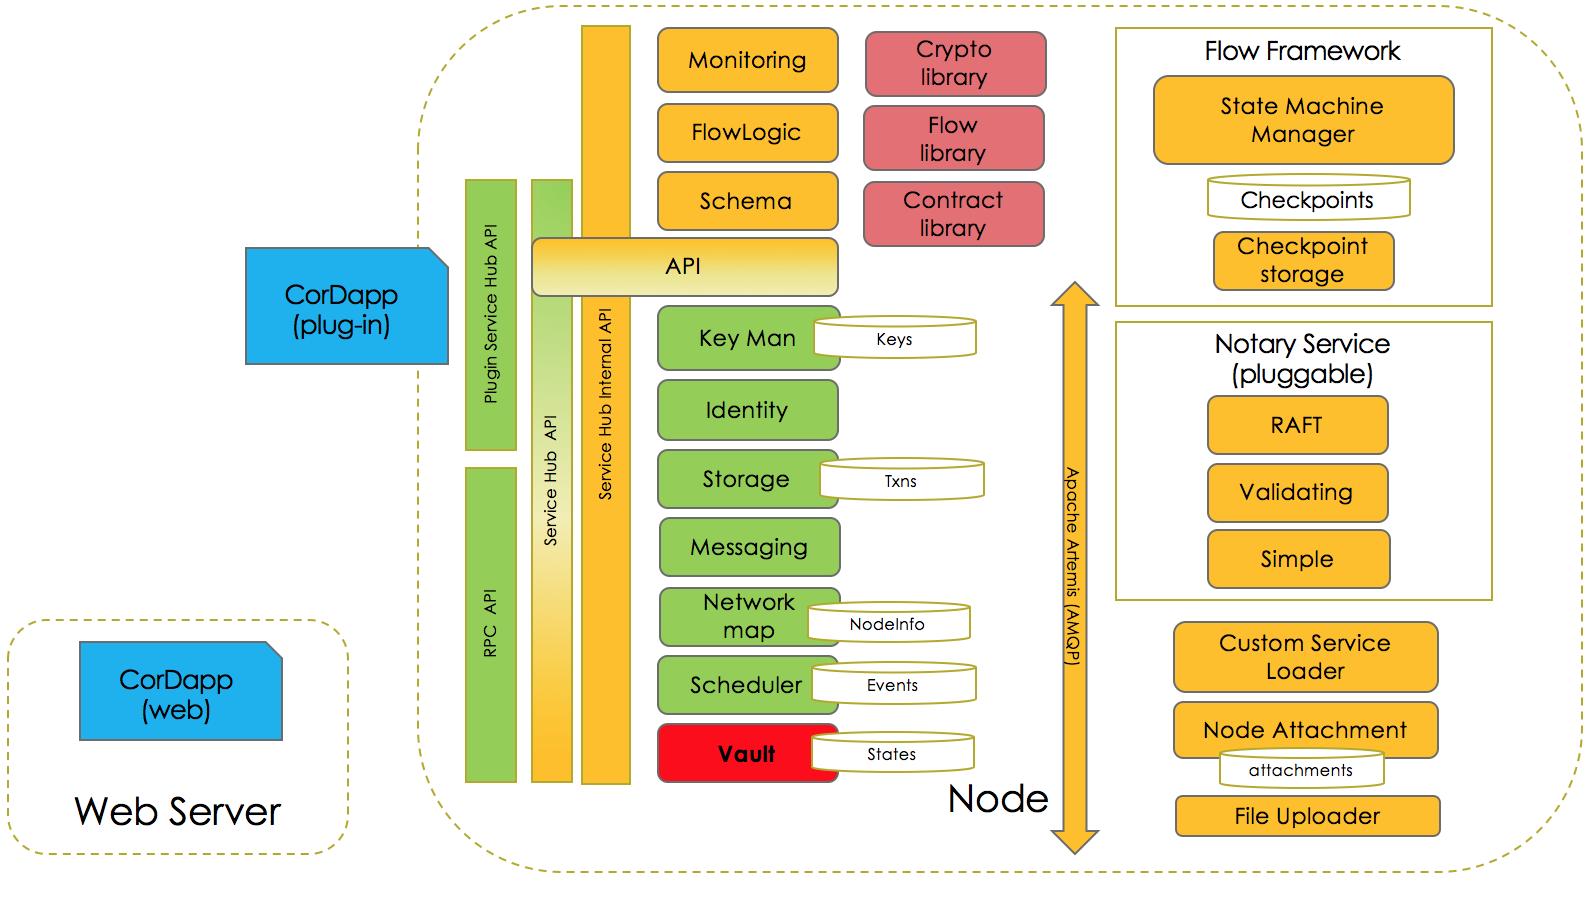
\includegraphics[width=0.95\textwidth]{design.png}
\caption{General architecture of the Corda ecosystem \cite{fig:design}}
\centering
\label{fig:design}
\end{figure}
\\ \\
We can observe the notary services which can be pluggable consensus algorithms and can be different depending on the needs of each part of the system (for example, we might choose to have a RAFT notary running on the subsystem of nodes of one company, but have a validating notary for external transactions). Data is shared on a need-to-know basis, so that the dependency graph of a transaction is provided to another node on-demand. Notaries follow this ideology as well when validating transactions - they do not need to know the underlying contents of the transaction, they can just cryptographically verify them.
\\
All communication takes the form of small multi-party sub-protocols called flows, which can perform different tasks and send information between multiple parties. With them, parties can perform or request notarisation, membership broadcast, transaction resolution and recording. While flows define the business logic for the actions parties can perform, smart contracts define the business logic of specific assets. Flows use smart contracts to define and manage states. These are used throughout the project, either by modifying existing flows (like the \verb|TwoPartyTradeFlow|) or creating purpose-built flows for bilateral trading and auditing.
\\ \\
\begin{figure}[!htb]
\centering
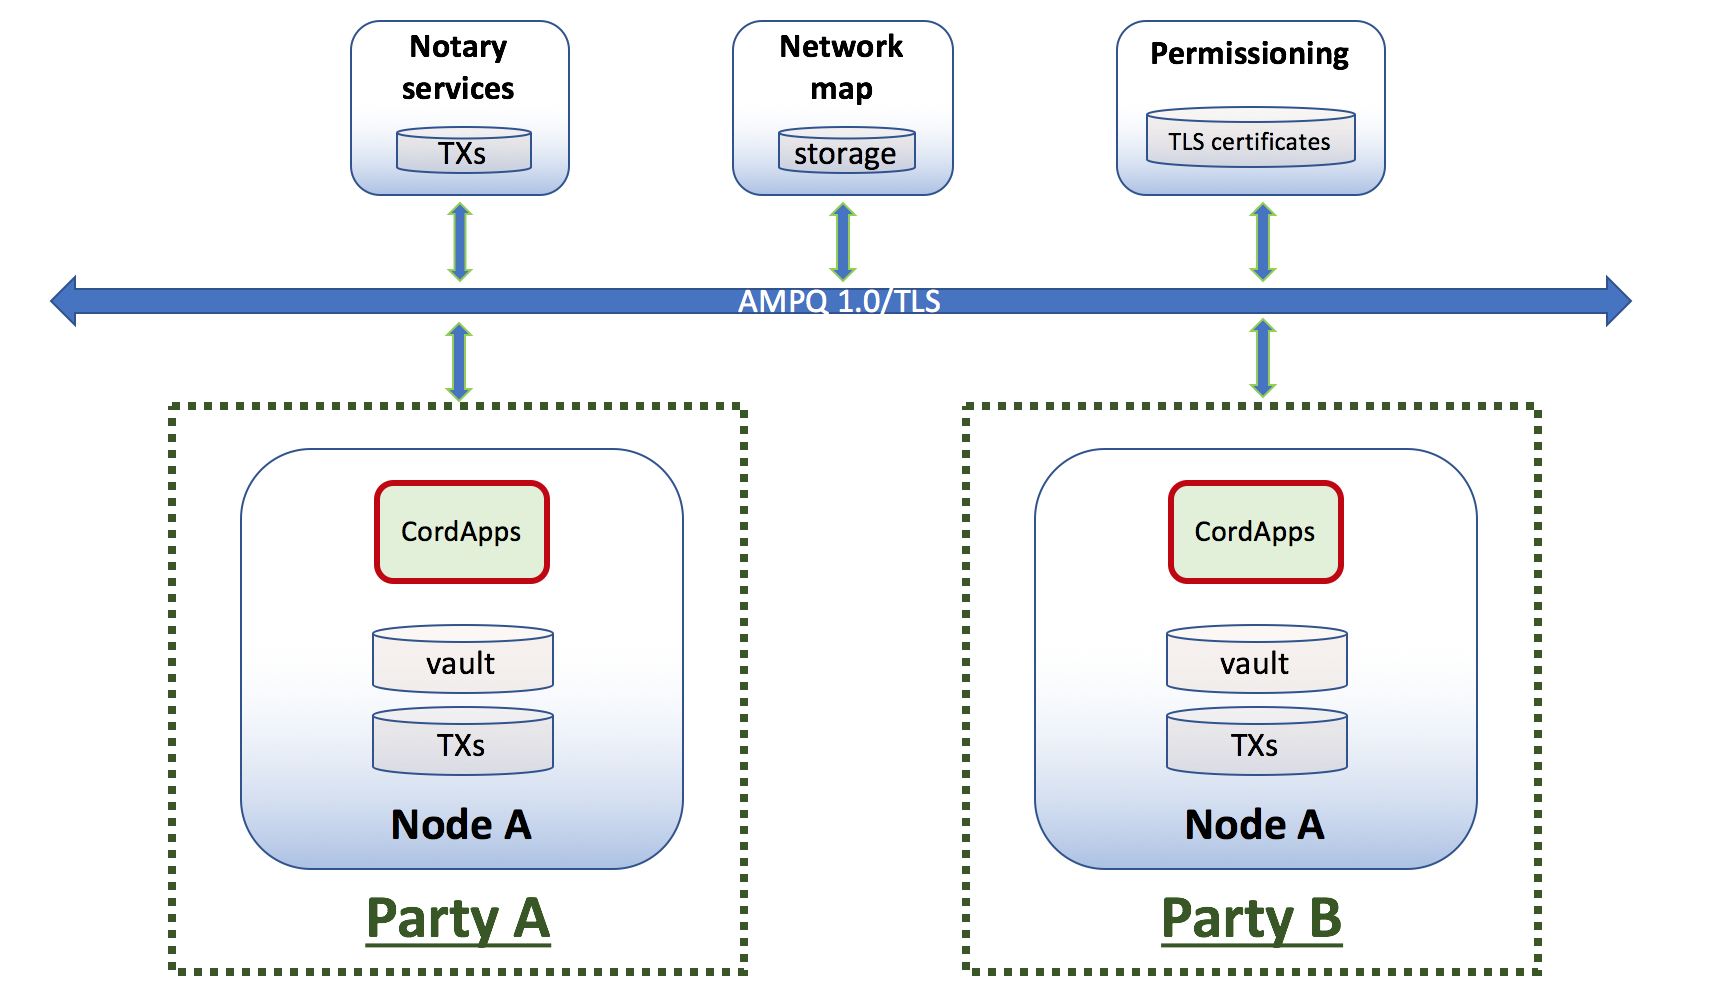
\includegraphics[width=0.8\textwidth]{designnode.png}
\caption{Inter-node communication structure \cite{nodestruct}}
\centering
\label{fig:system}
\end{figure}
\\ \\
Nodes also have remote procedure call APIs that aid interaction between different nodes and service hub APIs that offer information about the system the node is part of (notaries, regulators, vault access). Finally, there is a webserver provided so that Corda applications can service different sites depending on the features of the application. All these are part of the network, which looks like the the one in Figure \ref{fig:system} and shows how the nodes interact with each other in the larger eco-system. To be able to create this system of nodes, we first have to deploy them - this means creating a folder for each node, according to the rules defined for the component we are using. While in the final version, all the features would be merged together, currently we have packages defining different behaviours on different nodes. For example, the samples package offers some demo examples like a portfolio valuation demo or an application which performs interest rate swaps. We have used the trader-demo as the skeleton for this project. Once we have our nodes (either the general ones or application-specific ones), we have to start them up - registering them with the network map and establishing the port connections.
\\ \\
The four main concepts used throughout this project are states, contracts, transactions and flows. \textbf{States} will extend the \verb|ContractState|, which is the base class for every state that is present on the ledger. It contains a reference to the \verb|Contract| details and the participants, which are basically the parties from the network that can consume the state. A \textbf{LinearState} is a state representing a ``shared fact" which evolves over time. For example, we could represent a bond state with this state, given that we would have different changes to the value of the contract throughout its life. \textbf{OwnableStates} are states representing fungible assets like oil or gold, along with their current owner. We predominantly make use of these when we deal with cash states and the modifications they suffer.
\\ \\
\textbf{Contracts} define the business logic of a specific object, determining whether transactions are valid. They have a reference to the legal prose, stored as a hash for posterity in case of a legal challenge over what happened to a transaction. They also contain the \verb|verify()| methods, which check transactions for their internal validity.
\\ \\
\textbf{Transactions} are the objects transferred across from one node to the other in an attempt to perform a trade. Their life cycle follows a pre-determined course. We start by having a \verb|TransactionType.General.TransactionBuilder| which is a mutable container for any sort of transaction we might perform. We can add items (like states and commands) to the builder and we can sign it with a \verb|KeyPair| digital signature. Once we decide the transaction has all the required input and output states, along with the commands used to identify the type of transaction, we convert the \verb|TransactionBuilder| into am immutable \verb|WireTransaction|. Depending on the contract type and requirements, we have two options for a \verb|WireTransaction|. The first one is to have it signed by other parties - we would convert it to a \verb|SignedTransaction| which allows for digital signatures to be added to the transaction, based on checks performed beforehand, and then turn it into a \verb|LedgerTransaction|. The second one is to skip the additional signatures and convert it directly to a \verb|LedgerTransaction|. This type of transaction can be checked for contract validity before being committed to the ledger - an irreversible operation.
\\ \\
\textbf{Flows} are the actions that nodes perform to achieve different things - cash or asset issuing or trading, by exchanging messages among themselves. A \verb|FlowLogic| represents the actions executed by one side of the flow. Its \verb|call()| method defines the actions it has to perform - creating transactions, signing them, modifying them and sending them to the other nodes. To send information over to the other side of the flow, we would use the \verb|send()| method (which has an opposite \verb|receive()| method used on the receiving side). During flow execution, we have access to internal information about the node we are currently performing the actions from - the \verb|serviceHub|.
\\ \\
The \textbf{Service Hub} offers a flow all the information related to other nodes, the vault, past transactions and others. To retrieve information about other nodes' characteristics (i.e. to find notary or regulator nodes, to get a node instance from a string or to retrieve the name of a node from its IP), we can access the \verb|networkMapCache|. The storage for both the current and historic states of the node is found in the \verb|vaultService|, while additional information about transactions (like legal prose attachments) is found in the \verb|storageService|. To manage the node's digital signing keys (either searching for previously used keys or generating fresh ones), we use the \verb|keyManagementService|. 
\\ \\
The Corda system is organised under different packages. The most important ones to this project have been the core, finance and node ones. In the \textbf{core} package, we have the definition of different utilities, along with the cryptographic libraries used throughout the system and some of the messaging infrastructure. We also find the core RPC operations here - the methods that the node exposes to clients using the Java client library. This is where we need to add code to implement any vault operation - getting available shares, retrieving spendable cash or other consumable states. This package also defined the transaction types and the builder which we will use throughout during our flows.
\\ \\
In the \textbf{finance} package, we find a library of implemented contracts and some flows. In this place, we add our share contract definition, used for trading stock between nodes. Since cash (as a digital currency) should only be introduced on the ledger through a Central Bank authoritative node which has a special set of permissions, we use a mock entity in our project called Bank of Corda. The flows from this package define behaviour such as cash issuance, payments and exiting, which are used in conjunction with the Bank of Corda entity. 
\\ \\
The \textbf{node} package contains all the utilities employed to make the node run. These range from key management facilities and event management functions to database configurations. This is also where the \verb|FlowStateMachine| is implemented - this instrumentalises the flow logics and delegates actions to different nodes, depending on the behaviour requested. Considering we have multiple types of nodes in the system, this package defines each type - market participants (which are the basic transacting nodes), regulator nodes (with auditing facilities) and notary nodes (either a simple non-validating one or a RAFT or BFT-SMaRt cluster).
\\ \\
While additional applications are meant to be created as separate CordApps, we considered the work of this project more appropriate to be included in the basic code, hence the changes made were applied directly to the core codebase. While most of the work particular to trading was carried out in the \textbf{samples} package, we have touched upon all of the previously mentioned packages. Extending Corda in its current state proved very difficult because there are some tight couplings between different classes and modifying behaviour managed to break other features. One such example was a flow directing the actions between two nodes that were performing a trade. While this should be a generic flow (being able to trade any asset in return for another asset of similar value), it only implemented a currency versus simple asset swap. Therefore, the work carried out took into consideration the modifications brought onto the system as a whole and attempted to minimise any potentially disruptive behaviour from newly implemented classes and objects.
\newpage
\section{Implementation}
\label{sec:DesignImplementation}
For the implementation of the project, we have worked on the M10 version of Corda and the M9.1 version of the CordApp template. The creation of new features such as contracts and flows followed the structure that was present in the system to retain the familiarity for others who might extend the codebase further. 
\subsection{The \textit{ShareContract}}
\label{sub:Contract}
Contracts define the business logic of an asset. Since our goal is to be able to trade shares in Corda, we first have to build a contract expressing this asset. A well-defined contract presents the state of the asset - who issued what, when and at what price. In this new contract, we have a data class defining the state of the shares. This contains references to the \verb|issuance| (the party that initially issued the share - the exchange it was generated from), the \verb|owner| (representing the party which currently has the given share contract in their wallet), the \verb|faceValue| (the amount at which the shares were traded when the contract was created, used mostly for reporting purposes), the \verb|maturityDate| (used for timestamping reasons, it is usually right the instant of the trade), the \verb|qty| (the number of shares traded in the given contract) and the \verb|ticker| (the reference to the company whose stock we are trading). This extends the \verb|OwnableState| - like cash, shares are fungible and it does not matter whether they traded at different prices as long as we have them in our vault.
\\ \\
To be able to use the underlying infrastructure, new contracts should be defined by implementing the \verb|Contract| interface, a serialisable structure that defines business logic on the ledger. This means that every new contract we create must have a \verb|verify()| function, which is called every time a transaction involving the contract occurs. Participants to a trade call this function for every \verb|LedgerTransaction| they see on the network. This checks the internal details of the contract and whether every requirement is satisfied. For example, the verify function should check the timestamp, check whether the right amount of cash is being sent and check the correctness of the owner, as well as many other smaller checks. We have a separate \verb|verify()| function for each clause a contract defines: whether it's an issue, move or transfer.
\\ \\
For contracts to be registered on the ledger, we need to have a way of recording them. Since contracts are stored in the node's database, we need a new database schema representing a share. This is similar to existent schemas representing commercial papers, with the addition of the ticker symbol and the quantity. Each node's database will contain a table representing the shares it owns (using the schema that can be observed in Figure \ref{fig:schema}).
\begin{figure}[!htb]
\centering
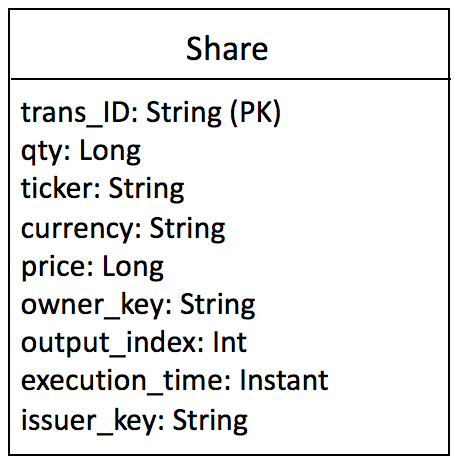
\includegraphics[width=0.4\textwidth]{schema.png}
\caption{Implemented schema for the share contracts}
\centering
\label{fig:schema}
\end{figure}
\\ \\
To see this in action, we can look at the state of the database in one of the nodes, after a few trades have been performed. This is shown in Figure \ref{fig:db}, where we can notice the output index, as \textbf{OUT}, defining the state of the shares. If the index is zero, it means that contract has been not been consumed, and is still in the possession of the current node. If the index is not zero, it means the contract has already been traded and the only reason why it is being kept in the database is for reporting reasons. To be noted that the transaction ID and the participant keys have been shortened for demonstration purposes.
\begin{figure}[!htb]
\centering
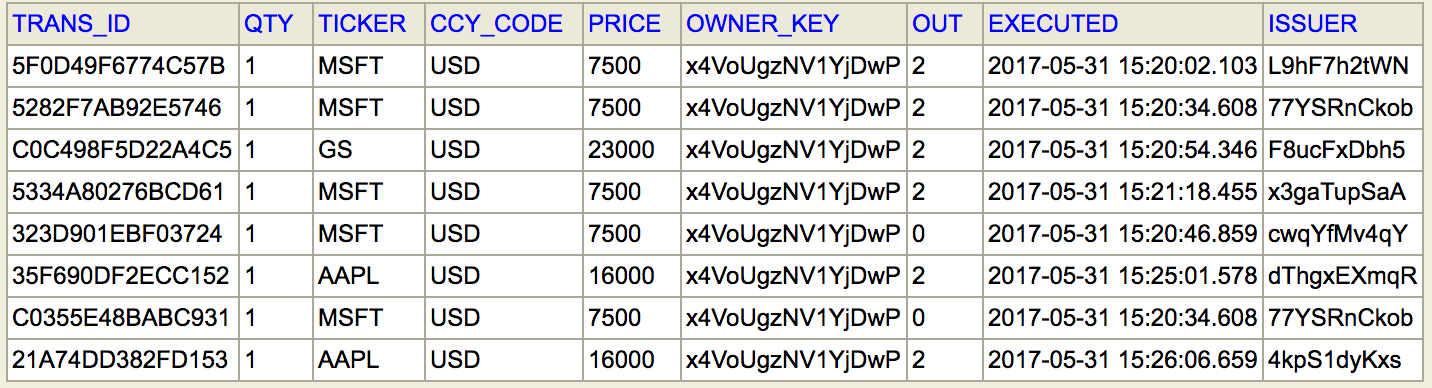
\includegraphics[width=1\textwidth]{db.png}
\caption{Example of the state of the database after performing some trades}
\centering
\label{fig:db}
\end{figure} 
\\
The next building block for our new contract is defining the required clauses. These are the actions that an agent can perform with a given contract. For a \verb|ShareContract|, there are three main actions: issuance, movement and transfer. The \textbf{issuance} is performed at the beginning of the share contract cycle and should contain the details of the initial issuer. This action would generally be performed when the shares are put on the market, by an authorised participant. The \textbf{movement} is performed after the issuance, when the authorised seller moves the shares to one of the participant nodes. While similar to the transfer, the movement is meant to be used in mocked approaches to populate the ledger. The \textbf{transfer} is the essence of the contract, performing the ownership exchange between the buyer and the seller, trading cash for assets.
\\ \\
For each command, there is a \verb|verify()| function as mentioned before. We can verify a plethora of requests according to the business rules, however, to simplify the understanding of the system, only a few important ones have been implemented. As examples, we have requirements like \verb|correct price for contract|. This verifies whether the money being sent over accurately matches the price of the share, as reported by an internal system. This is shown in Listing \ref{l:issue}, which describes the verify function of the Issue clause. To note that the verification checks currently performed are not exhaustive.
\\
\lstinputlisting[label = {l:issue}, language=Octave, caption = The verify function for the issue clause]{/Users/mikecar/Desktop/Blockchain-dizzy/imgs/issue.m}
To be able to present a realistic version of this verification, we have implemented a share price fetcher, that returns the real-time price of a given share from Yahoo! Finance. This retrieves the CSV file containing the requested details from Yahoo! using the finance quotes utility. We then parse the file to obtain the price which we return to the verify method. This would obviously be replaced by more performant reporting systems used in the industry (such as data retrieved from a company like Bloomberg). 
\\
In the case of a mismatch (i.e. when the amount of cash sent is smaller than the value of the share), the contract will report a verification failure and the transaction will not be carried through. While initially, we were requesting an equality relation between the two prices, we realised that there should be a threshold for price acceptance. In the real-world, trades do not usually happen at exactly the price reported by an exchange, so now the contract verifies whether the buyer of the asset is sending at least the amount of cash the exchange reports it should send.
\\ \\
Another requirement for clauses is found in the \textbf{move} and \textbf{transfer} ones. We want to keep the contract on the ledger by \verb|propagating| \verb|the| \verb|state|, so the transaction will have as output the contract as well, with some modified parameters. This differs from the CommercialPaper contract Corda implements, which instead of the \textbf{transfer} clause provides a \textbf{redeem} one. When the paper reaches maturity, its owner can redeem it for a higher amount of cash than the one initially paid. To perform this action on the ledger, we do not want to propagate the state - we want to dispose of the contract (the transaction having an empty output). While we could have modelled the share contract according to this ideology, it would have meant that for every transfer, we would first redeem the old contract, then issue a new one with a different owner. This is not appealing for a few reasons: it would involve more work done by the system (performing two commands instead of one) and it would provide complicated auditing facilities (instead of going through the transaction graph looking for one type of command (transfer), the regulators would be forced to search two types of commands and match them, increasing the complexity of the system).
\\ \\
However, to use these clauses on existing transactions, we need to define several functions. These will create or update a given transaction according to the business logic they define. We first have the \verb|generateIssue()| which returns a newly created transaction with the given parameters: price, ticker, quantity and owner (Listing \ref{l:genissue}).
\lstinputlisting[label = {l:genissue}, language=Octave, caption = Generating a share contract (from original codebase)]{/Users/mikecar/Desktop/Blockchain-dizzy/imgs/genIssue.m}
Secondly, the \verb|generateMove()| function modifies the owner of the contract in the transaction passed as a parameter (Listing \ref{l:genmove}). Finally, the \verb|generateTransfer()| would execute the shares-for-money exchange between two participants. Given the complexity of the transfer command, we have chosen to perform the asset exchanges within a flow rather than within the contract, especially since it involves more than one participant (for example, we need to both subtract cash from the buyer and subtract shares from the seller). This procedure is detailed in Section \ref{sub:transfer}.
\lstinputlisting[label = {l:genmove}, language=Octave, caption = Moving a share contract to a different owner (from original codebase)]{/Users/mikecar/Desktop/Blockchain-dizzy/imgs/genMove.m}
This contract is the basis of all the applications and flows developed in this project. It showcases delivery-versus-payment as well as ownership modification, proving that the clearing and settlement of trades could be done faster by employing this methodology.

\subsection{The flows}
\label{sub:TheFlows}
Flows represent the lower level network protocols that implement contract-specific business logic. These actions are performed sequentially, exchanging messages across multiple nodes. Since digitally signed transactions are used to update the ledger with the most current information, we need a way to perform the signing from each node, after we verify the correctness and completeness of the transaction. In theory, a \textit{continuation} is a ``suspended stack frame stored in a regular object that can be passed around, serialised, unserialised and resumed from where it was suspended" \cite{Corda:docs}. Although the JVM does not natively support continuations, Corda uses the Quasar library which implements them. Using continuations has several benefits: the code is free of callbacks (looks like sequential code), suspended continuations take up less space than suspended threads and abstracts away persistence and serialisation.
\\ \\
Suspendable functions (annotated by \verb|@Suspendable|) contain calls to send or receive methods - at this point, the flow framework will suspend the code and serialise it to disk. To be able to call the send-receive methods, the object being exchanged in the communication must be serialisable. A short discussion about any problems this requirement can present is done in Section \ref{sub:Flows}.
\\ \\
Some of the important flows that will be mentioned in the following subsections are the \verb|NotaryFlow|, the \verb|BroadcastFlow|, and the \verb|FinalityFlow|. The \verb|NotaryFlow| is called whenever we want to ascertain whether a transaction follows the set requirements for correctness. A snippet of what actions the notary would perform with this flow is given in Listing \ref{l:notary}.

\lstinputlisting[label = {l:notary}, language=Octave, caption = NotaryFlow code verifying transaction details (from original codebase)]{/Users/mikecar/Desktop/Blockchain-dizzy/imgs/notary.m}

Through this flow, the notary checks the transaction for correct timestamping, verifies whether the inputs given have been used in any other transaction (i.e. checks for double-spending) and checks whether the signatures on the transaction are sufficient for the it to be approved. When passing the transaction to the notary, only the minimum needed information is sent through, without any sensitive details.
\\ \\
The \verb|BroadcastFlow| takes a signed transaction (i.e. after it was signed by the participants and the notary) and broadcasts it to whoever needs to see it on their ledger. Usually, the transaction is recorded in the transacting parties' ledgers, along with the regulators' vaults. In some cases, we can add extra participants. For example, suppose Bank A and Bank B perform a trade, but Bank C is the ``parent" of Bank A and wants to oversee all their activity as well. In that case, we can add Bank C to the list of entities that will see the transaction. The \verb|FinalityFlow| is the higher abstraction of the two previous flows. It combines notarisation and ledger committing into one flow, broadcasting the transaction to all required entities. Once the finality flow is completed, the transactions are recorded on the ledger and the information cannot be modified any longer.
\lstinputlisting[label = {l:finality}, language=Octave, caption = FinalityFlow code notarising\, recording and broadcasting a transaction (from original codebase)]{/Users/mikecar/Desktop/Blockchain-dizzy/imgs/finality.m}
Because of the way messages are exchanged between the two parties participating in a trade, flows are started in a counter-intuitive way - the first party to initiate contact is actually the \textbf{seller}, not the buyer as in the normal trading situations. Since the project is creating a reporting facility, this does not influence any performance of actual trading. The price negotiations are done \textit{outside the system} and the trades are being input into the ledger only once the terms have been mutually decided by the two parties.
\subsubsection{The \textit{Issuer Flow}}
\label{sub:issuerFlow}
To be able to perform a trade, we first need to have capital. Although introducing cash on the ledger is a problem discussed in more detail in Section \ref{sub:cashissuers}, especially from a regulatory point of view, we do require nodes to have some money in their vaults to be able to transact later on. One solution is to utilise the mock version of a cash issuer, called \verb|BankOfCorda|. This is meant to act as a Central Bank, issuing cash for the parties in the system (without any pre-requirements). Of course, since this is just a demonstrative example, we allow every request for cash to be fulfilled, regardless of the amount a node asks for. 
\\ \\
Although the \verb|IssuerFlow| is meant to be used to issue different assets, the current implementation is particularised for the issuance of cash only. The project has used this flow as-is, without modifying its structure or business logic. To issue the cash, we have to request an amount in a given currency - we will get back \textbf{cash states} as opposed to just an integer representing the amount in a specific currency. This is related to the fact that cash is used in contracts, therefore we need to have usable states for the transactions. The way the flow is called in our applications can be seen in Listing \ref{l:cashissuance}.
\lstinputlisting[label = {l:cashissuance}, language=Octave, caption = Example of calling the issuer flow which populates a node's vault with cash states (from original codebase)]{/Users/mikecar/Desktop/Blockchain-dizzy/imgs/cashissuance.m}
The guideline for cash requests is to ask for several randomly sized amounts that sum up to the total required amount. This should be done because of the way cash is extracted from the ledger. Each of the requested amount is submitted for parallel execution, each of them calling the \verb|IssuanceRequester| clause of the \verb|IssuerFlow|. Once all the threads have finished and returned, the buyer has its vault filled with mocked-up cash. Since cash is being stored in smaller chunks instead of having a big pot of money, there is a heuristic to decide how to spend money. Whenever we consume cash from our vault, we need an input state to confirm this in the transaction (as opposed to the operation being just a simple subtraction from the vault). 
\\
\begin{figure}[!htb]
\centering
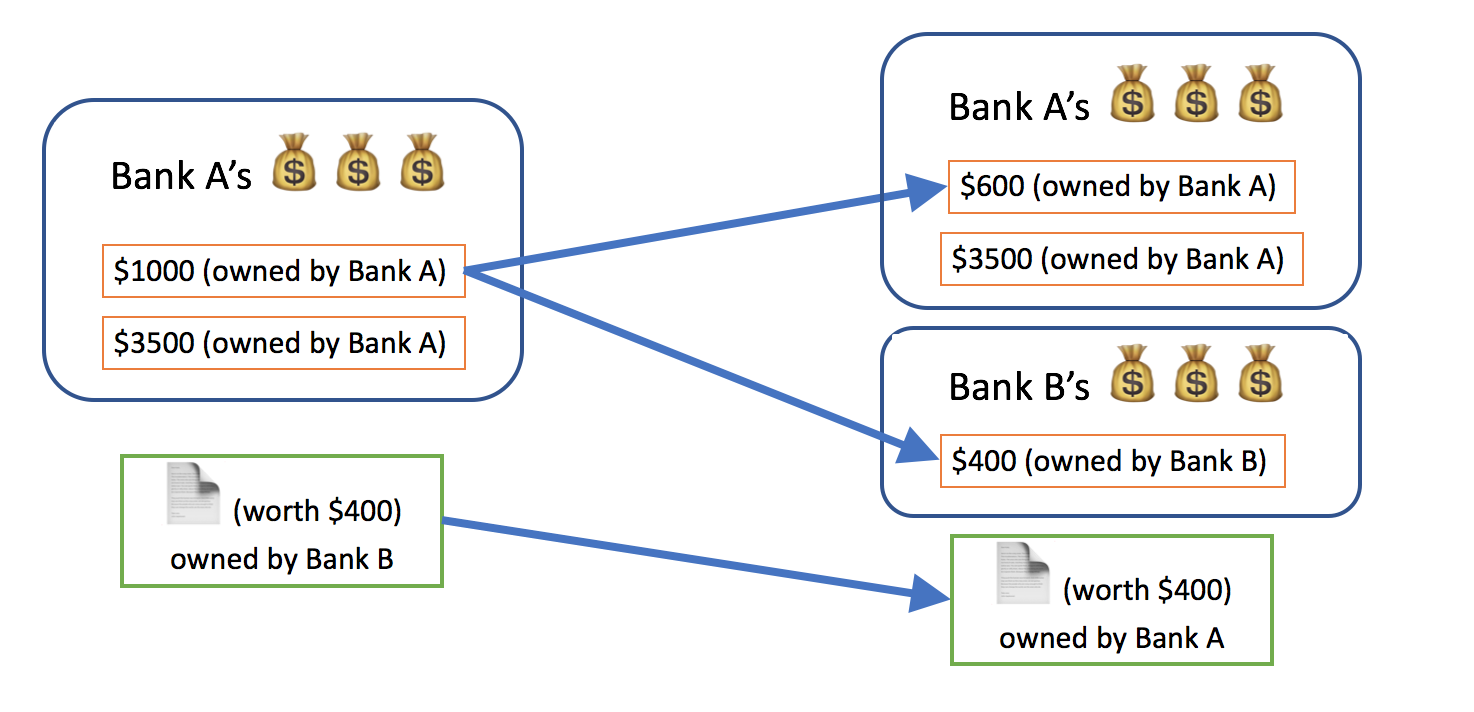
\includegraphics[width=1\textwidth]{cashspend.png}
\caption{Splitting cash states for change}
\centering
\label{fig:cashspend}
\end{figure}

An example can be seen in Figure \ref{fig:cashspend}. Suppose we are starting with two cash states in our vault (S1: \$1000 and S2: \$3500). The asset we are planning on buying is worth \$400. We find the first cash state that satisfies our requirement of containing at least \$400, which is S1 and we add it as an input to our transaction. However, we still want to receive change from our state, otherwise the pricing would be wrong. So we basically split S1 into S1a and S1b, each worth \$400 and \$600, respectively. These will be our output states, with different owners - S1a is owned by the asset seller, while S1b is owner by its initial owner (the buyer). To generalise this, we need to add as many cash states as needed to fulfill the price requirement of an asset. If the amount is exact, the buyer will not receive any change (no output cash state will be owned by him). However, in the case that the sum is over the amount needed for the asset, one of the cash states will be split in two pieces, with two owners. A similar approach is taken with shares, as presented in Section \ref{sub:spending}.
\subsubsection{The \textit{TwoPartyTrade, Buyer and Seller Flows}}
The \verb|TwoPartyTradeFlow| is the main flow that is able to perform trades in the system. However, since it was mostly created for a particular trading example (i.e. selling a commercial paper) its infrastructure was not employing generic types and the verification methods were too contract-specific. Therefore, to be able to sell other ownable states like shares by using the same flow, a few modifications were made, while keeping the structure of communication. Ideally, we would make this flow applicable to even more situations by trading \verb|OwnableStates| for \verb|OwnableStates|, not just for a specific amount of currency.
\\
\begin{figure}[!htb]
\centering
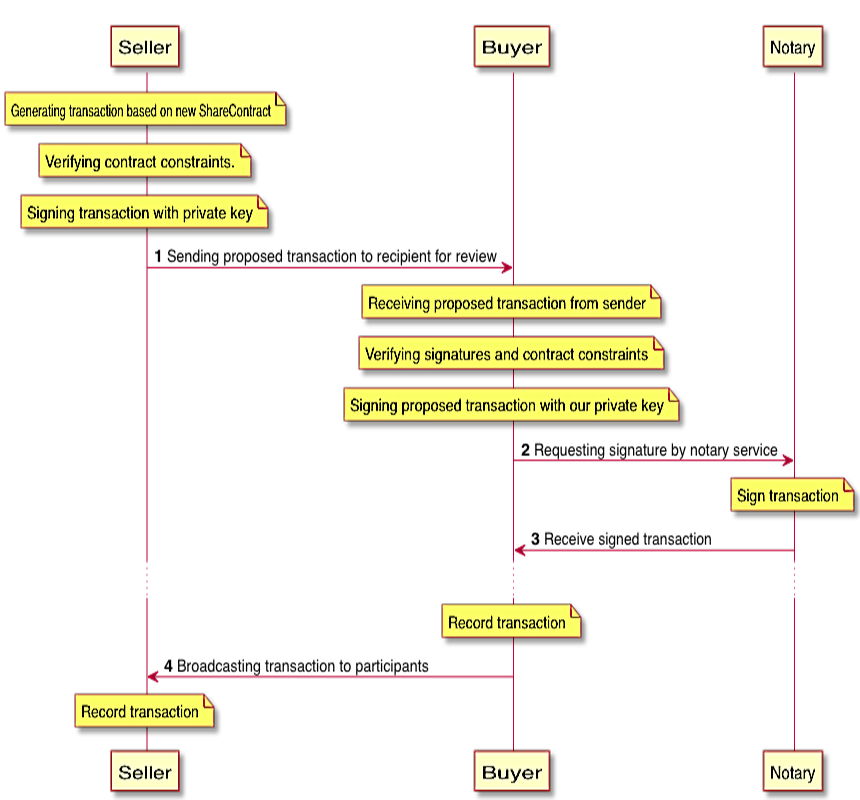
\includegraphics[width=1\textwidth]{tptf.png}
\caption{Two party trade flow sequence}
\centering
\label{fig:2ptf}
\end{figure}
\\
The individual \verb|Buyer| and \verb|Seller| flows are application-specific and they basically set up the trading terms before calling the delivery vs payment swap that the \verb|TwoParty| \verb|TradeFlow| executes. They were both vastly modified to fit the purpose of share trading. This swap has a straightforward depiction in Figure \ref{fig:2ptf}. 
\\ \\
As mentioned before, the seller is the one to make the first move. In this case, the seller acts as the exchange, generating shares as well. For the version of the seller that trades the shares it already owns, refer to Section \ref{sub:transfer}. First, the seller generates a \verb|ShareContract| with the details passed as parameters (through a \verb|generate| \verb|Issue()| call). The call to the seller flow can be made from several places: either from the command line (which delegates through to a Gradle task), from the webserver (which uses the web API) or from an IDE (for example for testing facilities, you can directly call the flow). 
\\ \\
Once we \verb|verify()| the contract's constraints and we sign it with the seller's private key, it can be sent over to the buyer side by suspending the current flow. The \verb|BuyerFlow| takes over which receives the details of the transaction and initiates the buyer clause of the Two Party Trade. What follows is an exchange between the two parties which performs several tasks, leading to a signed transaction which is returned to both the \verb|BuyerFlow| and the \verb|SellerFlow|. The buyer has to add as an input to the transaction the cash it will move out of its ledger. The seller does the same thing for the share contract the buyer will receive. The outputs are going to be the share contracts and the cash amounts. The process by which these are retrieved and divided from the vault is detailed in Section \ref{sub:spending}. 
\\ \\
After the transaction has been verified on both sides for internal correctness and signed by the notary for external correctness, the \verb|FinalityFlow| performs the ledger commit recording the transaction, and returns the final details of the trade. These are displayed from each flow and appear in the node's dashboard, as can be seen in Figure \ref{fig:transactionDetails}. The inputs are obfuscated for security purposes, so we can only see a hash of their content (i.e. the input cash and the input share contract). The cash splitting discussed in the previous section can be clearly observed (underlined in red - first part goes to the seller, the second one stays in the buyer's vault). The share contract is underlined in blue, showing that ten shares in the GS stock have been transferred to the buyer in that particular instant, for \$220 a share. Lastly, we can observe the balance of the buyer, printed at the end of the transaction, underlined in green. 
\begin{figure}[!htb]
\centering
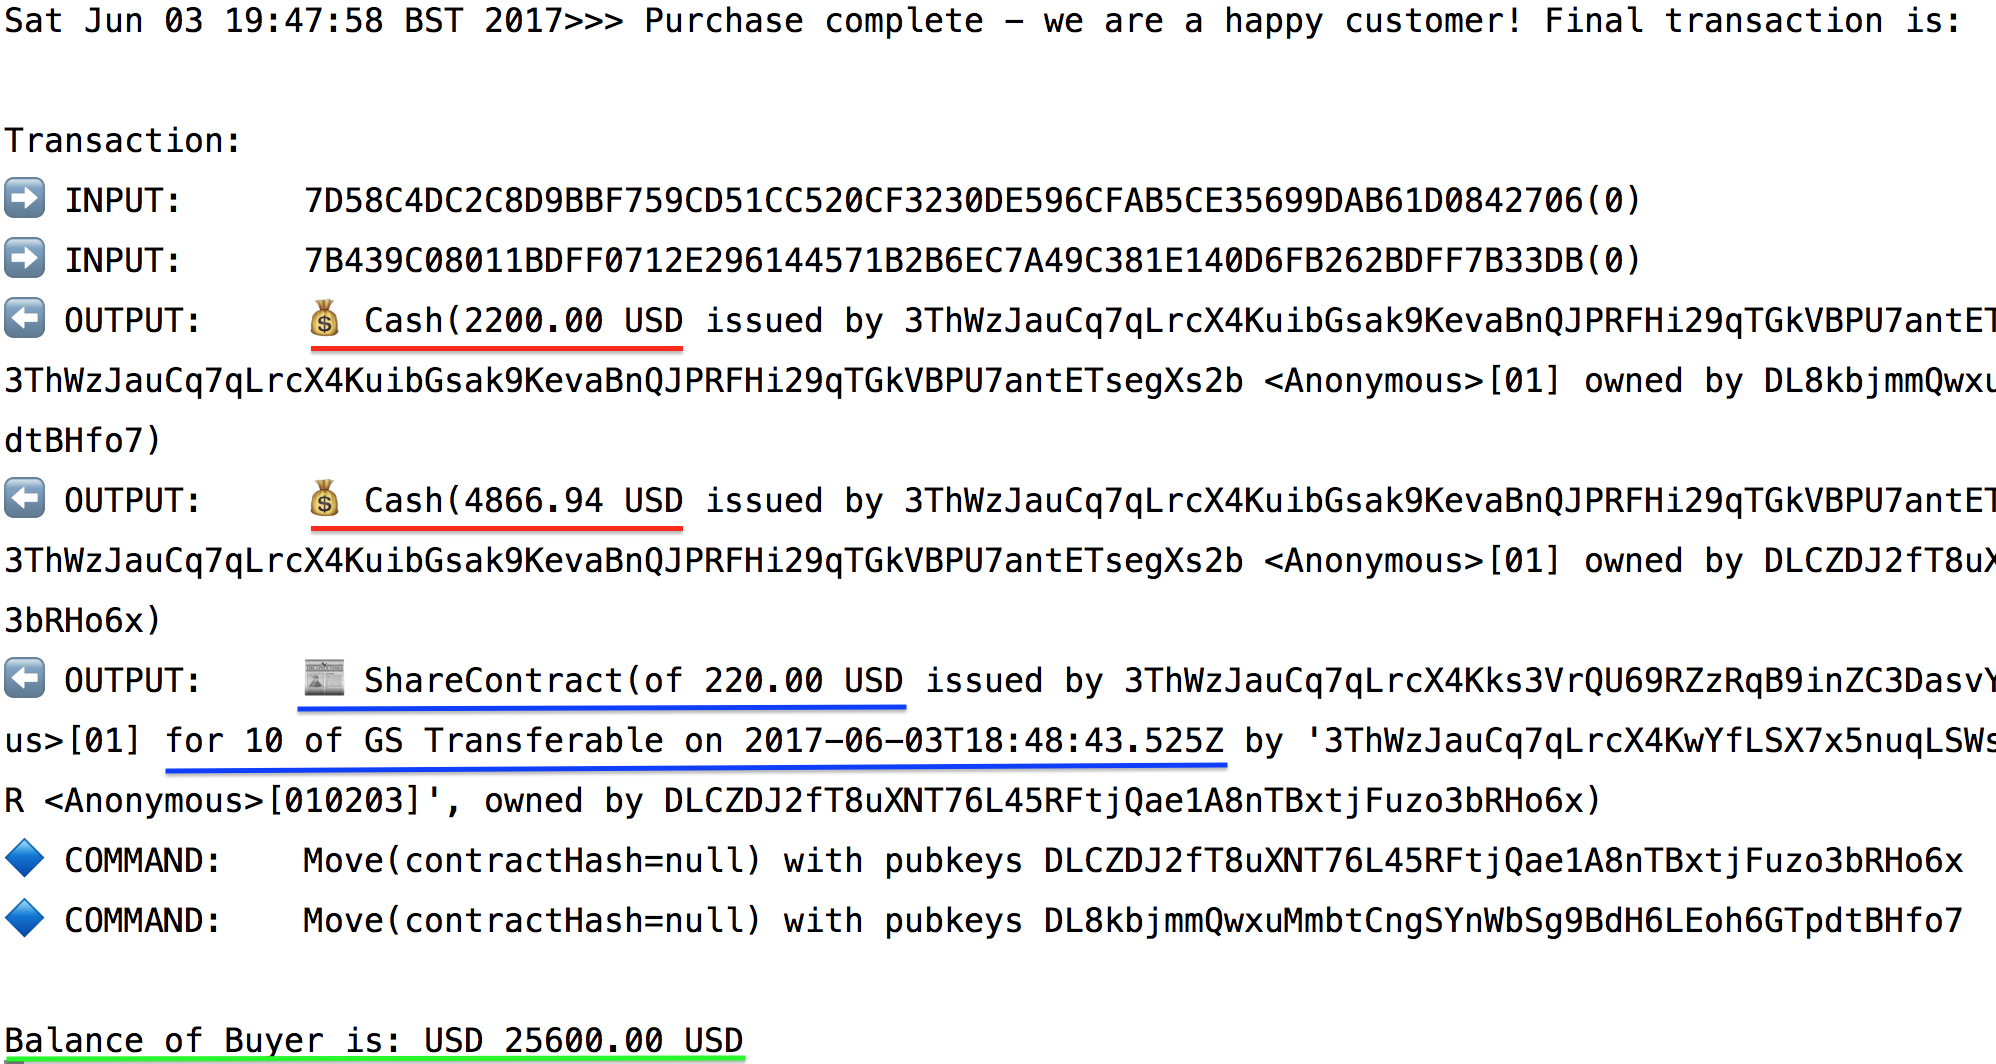
\includegraphics[width=1\textwidth]{transdet.png}
\caption{The resulting details after a TwoPartyTrade was performed with freshly-issued shares}
\centering
\label{fig:transactionDetails}
\end{figure}
\subsubsection{The \textit{Buyer} and \textit{Seller Transfer Flows}}
\label{sub:transfer}
At this point, we have all the infrastructure that permits us to populate the banks' vaults with assets, either cash or shares. The goal of the project is to be able to accurately represent trading between two parties in Corda. Although there are some building blocks available, they only partly emulate this trade (the \verb|TwoPartyTradeFlow| only deals with \textit{some} assets, without having a generic code and the \verb|SellerFlow| performs a sale by generating a contract on the spot, not by using the vault). The following flows have been fully implemented for this thesis, hence the reason we will go into more detail about what actions they perform and what were the challenges encountered.
\\
Firstly, to formally present the idea of the flows, we can think of Alice and Bob's trading idea that motivated this project. One of them has some shares, the other has some cash and they want to exchange the ownership of these (at a fair price). The difference in this case, as opposed to the \verb|SellerFlow|, is that we have to search our vault for the number of shares that we want to sell. This process follows a similar approach as the cash-splitting described in Section \ref{sub:issuerFlow}. We gather all the share states we need until we reach at least the amount requested, then we create two output states (one of shares going to the buyer, one of shares remaining in the seller's possession). 
\\ \\
Therefore, the \verb|SellerTransferFlow| adds the share-spending states to its transaction builder. The transaction builder will change throughout the flow, after additions of commands, states and signatures, until it matures into a \verb|SignedTransaction|. From the seller's side, after the states are added to the builder, we verify the contract for internal correctness and sign it with the seller's private key. Once this finishes, we require the signature from the buyer side as well (which means the flow has to suspend and delegate to the buyer). To perform this action, we use the \verb|SignTransferFlow| (briefly explained in \ref{sub:signtr}. At this point, the transaction on the seller side (for share spending) is complete and the last step remaining is running the \verb|FinalityFlow|. But, we need to create a transaction that will take care of cash as well. So we send the details needed to the buyer for it to deal with its side of the process. The call to send the details of the transaction to the other flow can be done at any point during the seller flow - it does not interfere with the processes that are happening on this side of the node. In Listing \ref{l:stf}, we can see that we have a send and a receive operation dealing with the cash transaction. These can also be replaced with a \verb|sendAndReceive()|, which has the same functionality.
\lstinputlisting[label = {l:stf}, language=Octave, caption = Code from the call method of the SellerTransferFlow]{/Users/mikecar/Desktop/Blockchain-dizzy/imgs/stf.m}
In the step where we are running the \verb|FinalityFlow|, we would eventually add the code to broadcast the transaction to the regulator nodes as well. The code for this should follow the pattern seen in Listing \ref{l:regs}.
\lstinputlisting[label = {l:regs}, language=Octave, caption = Broadcasting transaction to regulator nodes (from original codebase)]{/Users/mikecar/Desktop/Blockchain-dizzy/imgs/regs.m}
Once the \verb|BuyerTransferFlow| is called (by the \verb|send()| method in the seller node's flow), it receives the untrusted items from the seller. After thorough checks regarding the asset decided upon, prices and quantities (a snippet of the buyer's \verb|verify()| function can be seen in Listing \ref{verify}; this can be extended to include many other checks!), it begins its cash-spend transaction building process. 
\lstinputlisting[label = {verify}, language=Octave, caption = Verification checks for untrusted data received from the seller (in Kotlin)]{/Users/mikecar/Desktop/Blockchain-dizzy/imgs/code.m}
Using the same process as in the cash-splitting previously presented, it adds input and output states to the transaction, accurately representing cash movements. At this point, the transaction is verified internally by the buyer, then signed and sent to the seller for its own verifications and signature.
\lstinputlisting[label = {l:btf}, language=Octave, caption = Code from the call method of the BuyerTransferFlow]{/Users/mikecar/Desktop/Blockchain-dizzy/imgs/btf.m}
Once the confirmation is received, the two flows have \verb|SignedTransactions| in their possession, waiting for the \verb|FinalityFlow|. So the two finality flows are called, committing the transactions to the ledger. If one of the flows does not terminate successfully, the other one will be forced to roll back the changes as well, ensuring atomicity. 
\\ \\
Although a better idea would have been to create only one transaction with both the cash and the share inputs and outputs, there was an impediment. Communication between the two nodes is done with serializable items. To be able to create one transaction, we would have had two choices: start building the transaction in the seller, then send the builder over to the buyer to finish adding the rest of the details or send all the information to the buyer and let it build the transaction. The first idea did not work because the transaction builder is not a serializable object (the Kyro library that deals with serialization within Corda did not accept the \verb|TransactionBuilder| as a whitelistable class). Modifying the underlying structure of the builder was not appealing because of the other flows that were based around this structure. 
\\ \\
Therefore, we looked at the second option of sending all the required information over to the buyer (price, quantity, the share contract). The Kryo library required however to have all this information wrapped into a serializable data class. But again, the same problem happened as in the first case - the \verb|ShareContract| is not a whitelisted serializable object which meant that it could not be sent over to the buyer. After researching the serializable objects that can indeed be used, the only one that posed some interest was the \verb|SignedTransaction|. However, once a transaction reaches that level of maturity, it can no longer be internally modified - which means that if the seller sends a \verb|SignedTransaction| over to the buyer, it would not be able to add the cash states to it. 
\\ \\
The solution to the serialization problem was to create a data class containing only serializable attributes - the quantity, the ticker, the price and the public key of the owner. These would be needed for verifications in the buyer (is the price accurate for the share given? do we have that much money in our vault? is the quantity the same as what we requested?) and for the building of the cash transaction. 
\lstinputlisting[label = {l:ser}, language=Octave, caption = Serializable data class]{/Users/mikecar/Desktop/Blockchain-dizzy/imgs/ser.kt}
At the end of the flows, we have the confirmation for the transfer. Figure \ref{fig:innodeconf} shows the confirmation in the node's dashboard - we see the results after a transaction for 2 shares in AAPL, bought by Bank B. We can see the clear splitting of shares that took place (from an initial amount of 5 shares owned by Bank A) - the red underlined assets represent Bank A (which received \$320 and the change of 3 shares) and the blue ones represent Bank B (which received the 2 shares and the change from its randomly-sized cash state). Meanwhile, Figure \ref{fig:outnodeconf} shows the more succinct confirmation that appears on the machine that spawned the nodes (the same confirmation appears on the site, see \ref{sub:sharedEX}). This shows the transactions IDs, which can be used in the auditing phase described in Section \ref{sub:history}.
\begin{figure}[!htb]
    \centering
    \begin{subfigure}[b]{1\textwidth}
    	\centering
        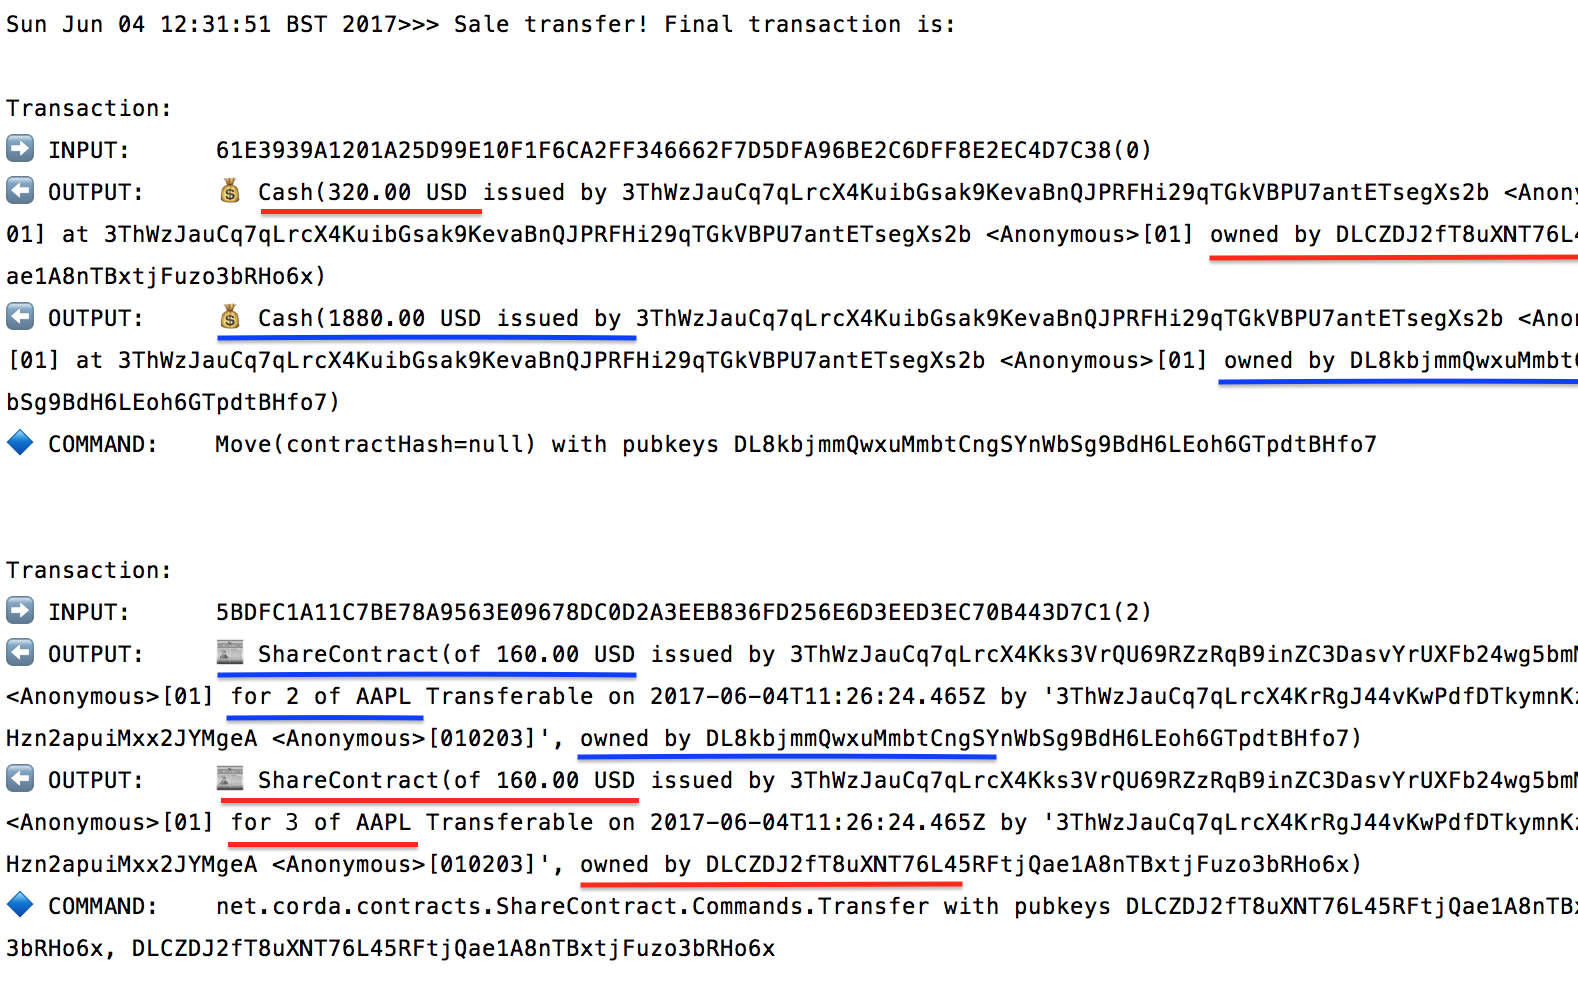
\includegraphics[width=1\textwidth]{innode.png}
        \caption{Confirmation in the node's dashboard}
        \label{fig:innodeconf}
    \end{subfigure}
    ~
    \begin{subfigure}[b]{0.8\textwidth}
    	\centering
        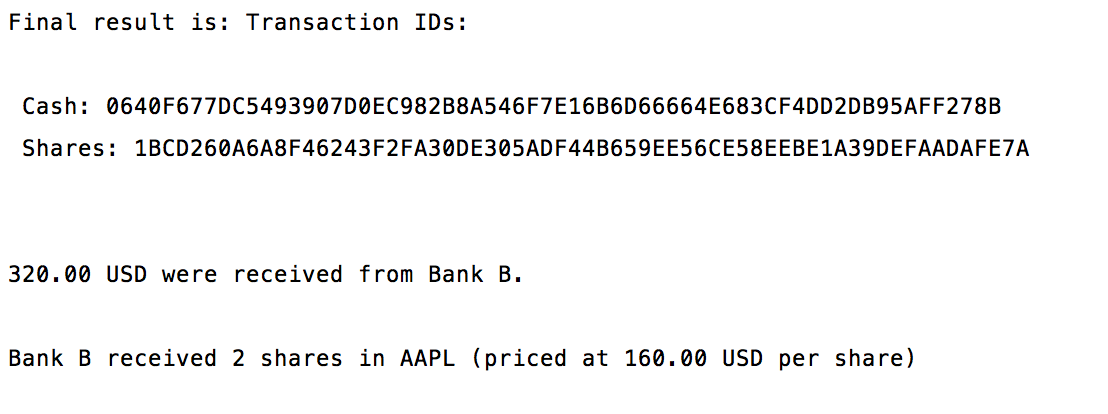
\includegraphics[width=1.2\textwidth]{outnode.png}
        \caption{General succinct confirmation (used for the site)}
        \label{fig:outnodeconf}
    \end{subfigure}
    \caption{SellerTransfer confirmations}
    \label{fig:confs}
\end{figure}

\subsubsection{The \textit{Signing Flow}}
\label{sub:signtr}
This flow automates the process of retrieving signatures from counterparties. Of course, whenever a counterparty gives its signature for a transaction, it evaluates the contents of the transaction for correctness from their side as well.
\\ \\
Whenever it is called, it gets as a parameter the transaction we are concerned with (which should be at least partially signed, by its creator). First, we verify this partially signed transaction according to the contract rules. Next, the flow determines who all the signers for the transaction are. Now, it has to convert the transaction into a \verb|SignedTransaction| by getting all the counterparties involved in the transaction to sign. Collecting the signatures involves sending requests to the respective parties and receiving their confirmation (or, if the party does not want to sign, cancellation). Once we check that all the signatures have been correctly received, we send the transaction to the notary for the final signature. The \verb|SignedTransaction| is now in its complete state and can be used further by the flow that called this Signing Flow.


\subsubsection{The \textit{History Flow}}
\label{sub:history}
One of the most important requirements for the system to be accepted by the industry was its ability to provide an infrastructure for compliance checks. The most common way this would be done is by looking at the transaction history and then, for each transaction, find out the details of when it happened, what the trade was about, who it involved and so on. For this to be possible, we defined a special-purpose node, called the Auditor. This is the entity that performs all the regulatory checks in our system. It acts in a similar way as the notary - flows can be called for the auditor, it is registered on the network map for every node to see and has a restricted usage (for example, the auditor cannot \textit{perform} trades, only oversee them). Moreover, just like we can have a group of notaries acting as one entity, the same thing applies to the auditors.
\\ \\
Although this is one of the main points discussed in the Corda whitepaper as well, the infrastructure for regulatory checks is not completely implemented. There are building blocks in place that signpost the progress made in this area. For example, there is a facility to traverse the transaction graph history looking for particular commands or states, but its functionality is very limited (currently, you can search for the initial issuance of a share). The network infrastructure is already in place, meaning that we can register the auditor node with the rest of the system. This enabled us to build a flow that would perform a similar operation to what the final regulatory implementation will do: find the details of a given transaction and examine its contents.
\\ \\
From the compliance point of view, this thesis is not concerned with the verification functions that an auditor has. However, the focus has been on accessibility of data - can we find the transaction if we know its ID? Does it show all the details that we need? What are the various possibilities to achieve this? Well, ultimately, the auditors will be added to each transaction as a passive participant - that is, the transaction will be broadcast to them even though they are not one of the parties contributing to the transaction. Once this is done, the transaction will appear in their vaults, but they will not have the option to use the states it contains. However, in the current system setting, the transaction broadcast does not send all the information necessary for the regulators. Although this will be eventually rectified, we wanted to determine if there is currently a way to work around this.
\\ \\
The idea is that if we have the transaction ID (which is the only information stored in the auditor's vault), we want to get the details of the transaction (which are stored in the participating nodes' vaults). The auditor cannot access the vaults of the banks directly (i.e. it cannot perform SQL queries on their internal databases). It can delegate this task to each node in the system, though. Then, the node would lookup in its own database whether it is in possession of the given transaction ID - if it is indeed, then it must return the details to the auditor. This is done by querying the vault for information on the transaction, which is stored in the \textbf{CONTRACT\_SHARE\_STATES} table. A snippet of the SQL query used for this flow can be seen in Listing \ref{l:query}. This querying tool is discussed in Section \ref{sub:query}, too.
\lstinputlisting[label = {l:query}, language=Octave, caption = Query extracting transaction information from the vault]{/Users/mikecar/Desktop/Blockchain-dizzy/imgs/query.sql}
There are tampering concerns in this setup - the bank could retrieve the correct transaction details but send bogus data to the auditor. This concern will be addressed in the future implementation of regulatory flows which will not depend on a node's trustworthiness since the data is kept on the auditor ledger as well (and cannot be tampered with). 
\\ \\
\begin{figure}[!htb]
\centering
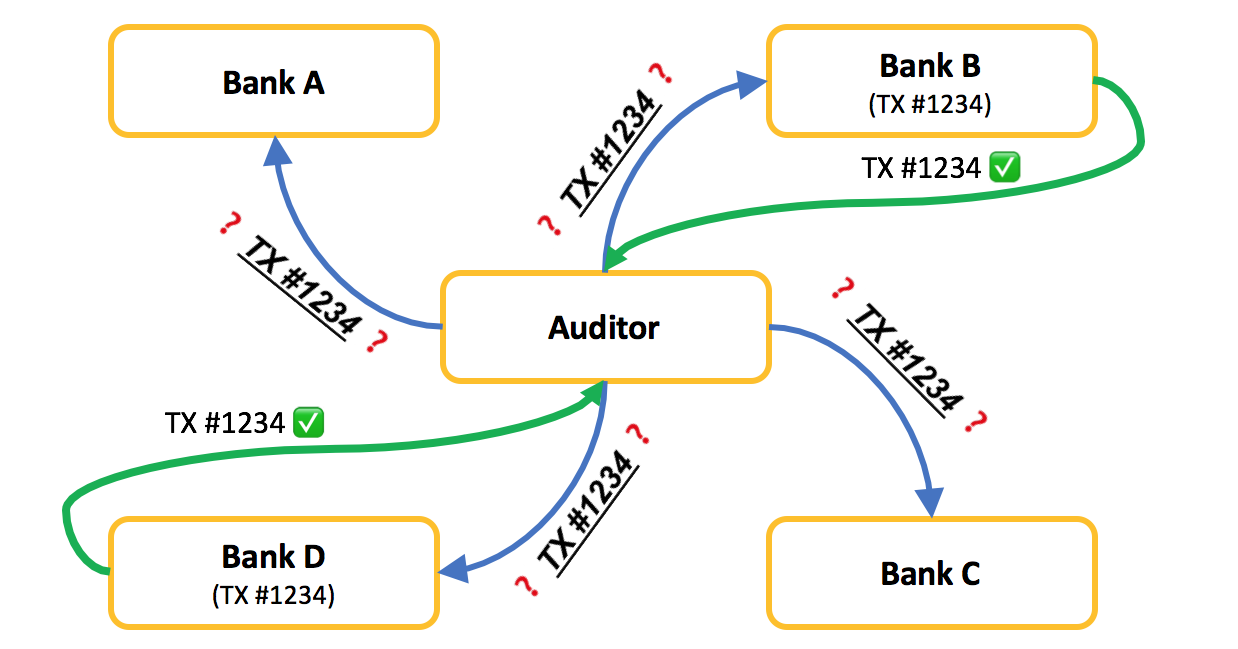
\includegraphics[width=1\textwidth]{audit.png}
\caption{The auditor's request for transaction details, along with the banks' response}
\centering
\label{fig:audit}
\end{figure}
\\
The history flow works by searching every node for a given transaction - this is visually depicted in Figure \ref{fig:audit}, where we see the regulator asking for the details of transaction \#1234 on the network (in blue lines). The regulator uses the information received from the first flow that returns the details (the green lines from Bank B and Bank D). In our system, we are currently just printing the transaction details (Figure \ref{fig:auditdetails}. In the real-world, the regulator flow would have a series of checks that it would perform to prevent against money-laundering practices or terrorist funding (AML and CTF rules \cite{amlctf}).
\\ \\
\begin{figure}[!htb]
\centering
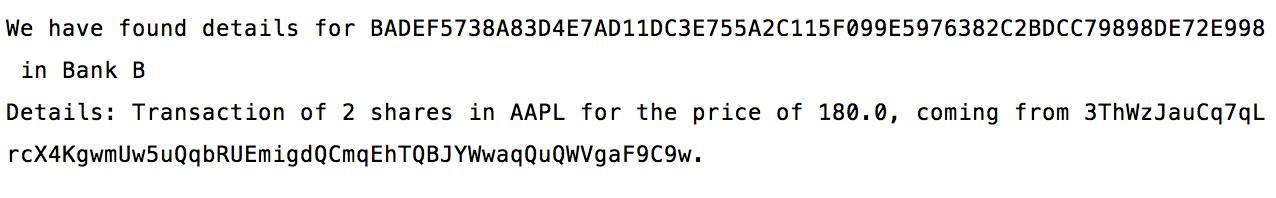
\includegraphics[width=1\textwidth]{auditdetails.png}
\caption{Minimal auditing details for a given TX ID}
\centering
\label{fig:auditdetails}
\end{figure}
\subsection{The Vault}
\label{sub:vault}
The vault, otherwise known as the wallet, holds all the information about the states that a node interacted with throughout its existence, both consumed and unconsumed. It stores the cash balances: a map of currencies to amounts, representing how much money an individual possesses in each currency. It also stores all the share contract states: contracts that specify how many shares of a company the individual has or had (because we keep recording the contracts that have been used, for posterity). The vault can be queried for information, either by accessing some of its fields (\verb|cashBalances| being a good example of this) or by performing SQL queries retrieving answers to specifically directed questions (``how many shares in stock X do I own?" or ``what are the stocks i have a stake in?").
\\ \\
Since accessing the vault essentially represents a database transaction, there have to be measures put in place so that the database's integrity is maintained at all times. Whenever we read or write to the database, we use a \verb|ReentrantLock()| to prevent inconsistencies. Whenever a transaction takes place, some states from the vault might get soft locked (for example, during a trade, a share contract might get temporarily soft-locked to prevent others accessing it; when the transaction finalises, the lock is removed and the state of the contract is modified accordingly - if it was used, it is converted into a consumed state, otherwise it remains as before). This represents a safety mechanism against dirty reads and writes.
\subsubsection{Querying the vault}
\label{sub:query}
To be able to perform the cash and share splitting aforementioned, we first need to retrieve their states. We can look initially at the \verb|unconsumedStatesForSpending| method in  \verb|NodeVaultService.kt|, which returns all the states that can be used to satisfy a given cash requirement. With the aid of an SQL join query, we retrieve all the spendable cash states in the vault. Going through the returned states, we make sure that the total cash balance is able to pay off the required amount. If that is not the case, we retry to get states from the vault - perhaps some state recently became spendable or unlocked (there is a maximum number of retries available). Otherwise, we successfully return the cash states that can be used. 
\\
A similar function for shares did not exist. Matters are mostly similar in this case, with one change - we group states based on their ticker and retrieve the summed up amount of shares for each. A sample of the states that exist in the database is depicted in Figure \ref{fig:shareStates} (cash states in \ref{fig:cash} and share states in \ref{fig:shares}). To be noted that the shares that have an \textbf{output\_index} of zero are unconsumed (constraint present in the SQL query for unconsumed states for cash/share spending).
\begin{figure}[!htb]
    \centering
    \begin{subfigure}[b]{1\textwidth}
    	\centering
        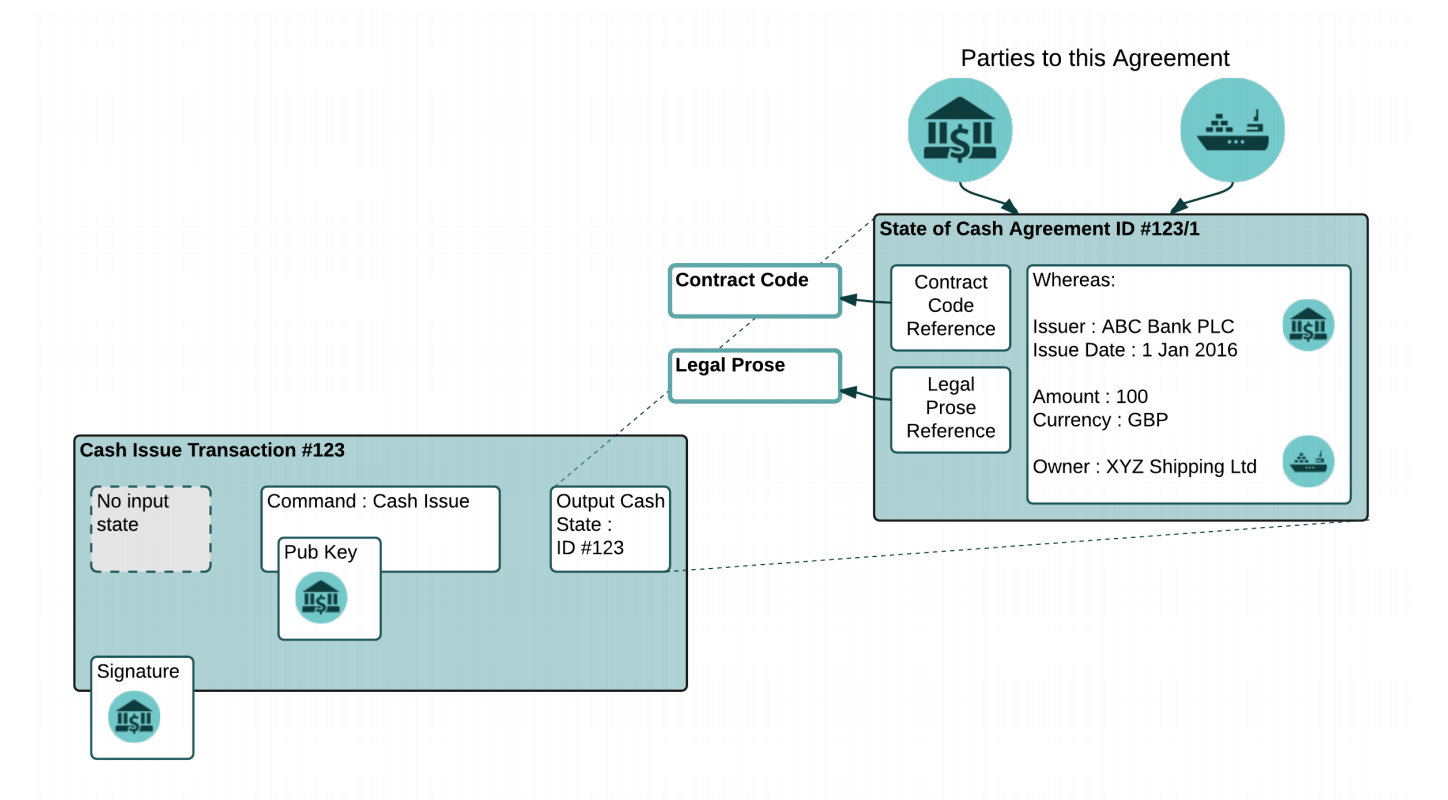
\includegraphics[width=0.6\textwidth]{cash.png}
        \caption{Cash states from a bank's vault}
        \label{fig:cash}
    \end{subfigure}
    ~
    \begin{subfigure}[b]{0.8\textwidth}
    	\centering
        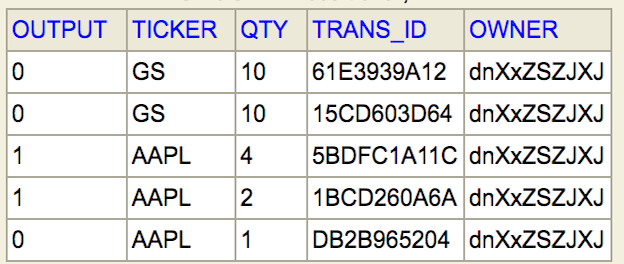
\includegraphics[width=0.75\textwidth]{shares.png}
        \caption{Share states from a bank's vault}
        \label{fig:shares}
    \end{subfigure}
    \caption{Vault contents, including already used states}
    \label{fig:shareStates}
\end{figure}
\\ \\
Another similar query we can make relates to a functionality created for internal visualisation of nodes - it shows exactly what the vault of a node contains (i.e. the balance and the shares it has). This display feature makes use of a vault access method defined in \verb|getShareBalances()|. We select the tickers and the quantity we have (accessible) in them. We only include spendable stock, as normal. The result of calling this method can be observed directly in the graphical example presented in Section \ref{sub:sharedEX}. 
\\ \\
Since all the transaction details are stored in the vault, we can access them at the auditors' requests. Given a transaction ID, we can determine the share contract that it is related to in the \textbf{CONTRACT\_SHARE\_STATES} tables. The \textbf{VAULT\_STATES} table stores information about the transaction IDs, hashes and participants, but no internal details, which have to be extracted from the share states table. If the select statement does not return anything, then the transaction does not belong to the current node. An exception would be when the node underwent some data loss and did not repopulate its vault with the backup data. Otherwise, if the select returns one row, then we can use the transaction details. To note that the select statement can actually return at most one row - transaction IDs are meant to be unique (since they are hashes). Hash collisions have no effect on nodes or auditor if they were to happen, because there would only be an exception in the regular 1:1 mapping of transaction ID to transaction details. 
\subsubsection{Share spending}
\label{sub:spending}
Share spending follows a similar heuristic as the cash splitting - we get as many share states as necessary, then split them into two: some go to the buyer, some go to the seller as change. The function that performs this is \verb|generateShareSpend()|, which gets as a parameter a transaction builder that will be modified during the execution of this method. We get the acceptable shares by calling the \verb|unconsumedShares| \verb|ForSpending()| mentioned above. This returns a list of ShareContract states that we need to peruse - the private method \verb|gatherShares()| acts as a check to verify whether the states we have are enough to sell the required amount of shares to the buyer. If they are, it gathers assets from the given list of states, sufficient to match or exceed the required amount. The method returns a pair which contains, on one hand the list of states and, on the other, the total amount of shares (which we need to know to be able to split the contracts). Since we use all the states from the list returned, we need to add them to the transaction builder as input states.
\\ \\
Now, for each state in the list of states, we deriving the share state by modifying the contract owner - this means that in this case, we change the ownership of share contracts \textbf{without creating new ones}. In the case that we have change to give back, we spawn two contracts depending on the amounts required. At the end, we need to add all the states (both the derived ones and the newly spawned ones) as outputs to the transaction builder. Since this call is made for a \textbf{Share Transfer} we are also required to add the \verb|Transfer| command to the transaction builder. This can be seen in Listing \ref{l:ss}.
\lstinputlisting[label = {l:ss}, language=Octave, caption = Generating share spends]{/Users/mikecar/Desktop/Blockchain-dizzy/imgs/gss.m}
\subsection{Gradle generalisations}
\label{sub:gradle}
Since we have discussed every building block needed for our applications, it is appropriate to explain the way the gradle tasks have changed since the beginning of the project. Initially, there were only three tasks available: deploying the nodes, the issuance call and the sale call. However, these had mostly hardcoded values: a specific amount of cash to be issued and only to a specific bank; the sale involved a commercial paper which had nothing to do with the way our project was heading and again, the two parties involved in the trade were hardcoded names for two market participants. Moreover, all the calls were made under the assumption that all the nodes are hosted locally, without having different IPs. An in-depth discussion about the network and the way nodes can actually be spread out over more than one machine can be found in Section \ref{sub:Nodes}.
\\ \\
To be able to perform complex trades, both from the command line and from a web interface, the gradle tasks had to be improved either by passing in parameters depending on each task or by determining different values (for example, the IP that a node is hosted on). We also improved the offer of gradle tasks available: we have the regular node deployer, but we also have a separate task that deploys nodes with webservers attached. We added a task for adding a node on-the-fly (Section \ref{sub:flynode}), a task for performing generic sales and generic trades, a task to display cash and asset balances of a node, two tasks that are control the random marketplace (Section \ref{sub:mkt}) and a task for auditing services. These can be found in the trader-demo package, in the \verb|build.gradle| file. A snippet from the gradle file can be seen in Listing \ref{l:rst} - the task which triggers a stock trade between two parties.
\lstinputlisting[label = {l:rst}, language=Octave, caption = Gradle task to trigger the seller transfer process]{/Users/mikecar/Desktop/Blockchain-dizzy/imgs/rst.m}
\subsection{The web interface}
\label{sub:web}
Especially in the development phase, flows are triggered by calling gradle tasks from the terminal. However, when the system goes into production, not everyone who will use it will know how to use a terminal, for example. Therefore, the need for an abstraction layer that hides most of the low-level work is needed. Some of the demos offered by Corda's creators have very basic web interfaces. The applications developed in this project also need such an interface, to open up the system and enable more people to use it than just programmers.
\\ \\
To enable this behaviour, there are a few components that need to be put in place. First of all, the node configuration needs to set up a web port, on a previously unused port number. Secondly, we need to specify which functions we are mapping to what URI - this is done by defining an API file (described below) and defining the directory from where web resources are being served. The API file defines several GET and PUT methods that are used throughout the webpage. Examples of these include the node's name GET method (Listing \ref{l:get}) or the PUT method that is called to sell shares (Listing \ref{l:put}). Some of these either access the node's vault or trigger a flow asynchronously.

\lstinputlisting[label = {l:get}, language=Octave, caption = Node name getter]{/Users/mikecar/Desktop/Blockchain-dizzy/imgs/get.m}

\lstinputlisting[label = {l:put}, language=Octave, caption = PUT method to sell shares]{/Users/mikecar/Desktop/Blockchain-dizzy/imgs/put.m}
From the front end point of view, we have an HTML file defining the structure of the webpage and an angularJS module which controls the behaviours on the page. For the former, the mentionable feature is the way it handles with different types of nodes - we want to have a clear differentiation between market participants (i.e. banks) and the exchange (which is only there to sell fresh shares to the other banks, since it cannot trade). This means that for each type of node, we have a different web interface - Figure \ref{fig:node} is displayed from a regular node's web server, while Figure \ref{fig:exch} is displayed from the exchange (which has no vault anyway). In the exchange's figure, you can see the details of the sale menu. A similar menu appears in the Bank's site when it wants to perform a trade, and this is further documented in \ref{sub:apps}. Even though there are exceptions in place on the back-end dealing with insufficient funds or shares, we have an extra layer of safeguarding. We cannot even attempt to sell stocks that we do not own. We cannot attempt to sell shares to entities that do not exist. We also cannot try to sell negative shares or shares of negative prices. 
\begin{figure}[!htb]
    \centering
    \begin{subfigure}[b]{1\textwidth}
    	\centering
        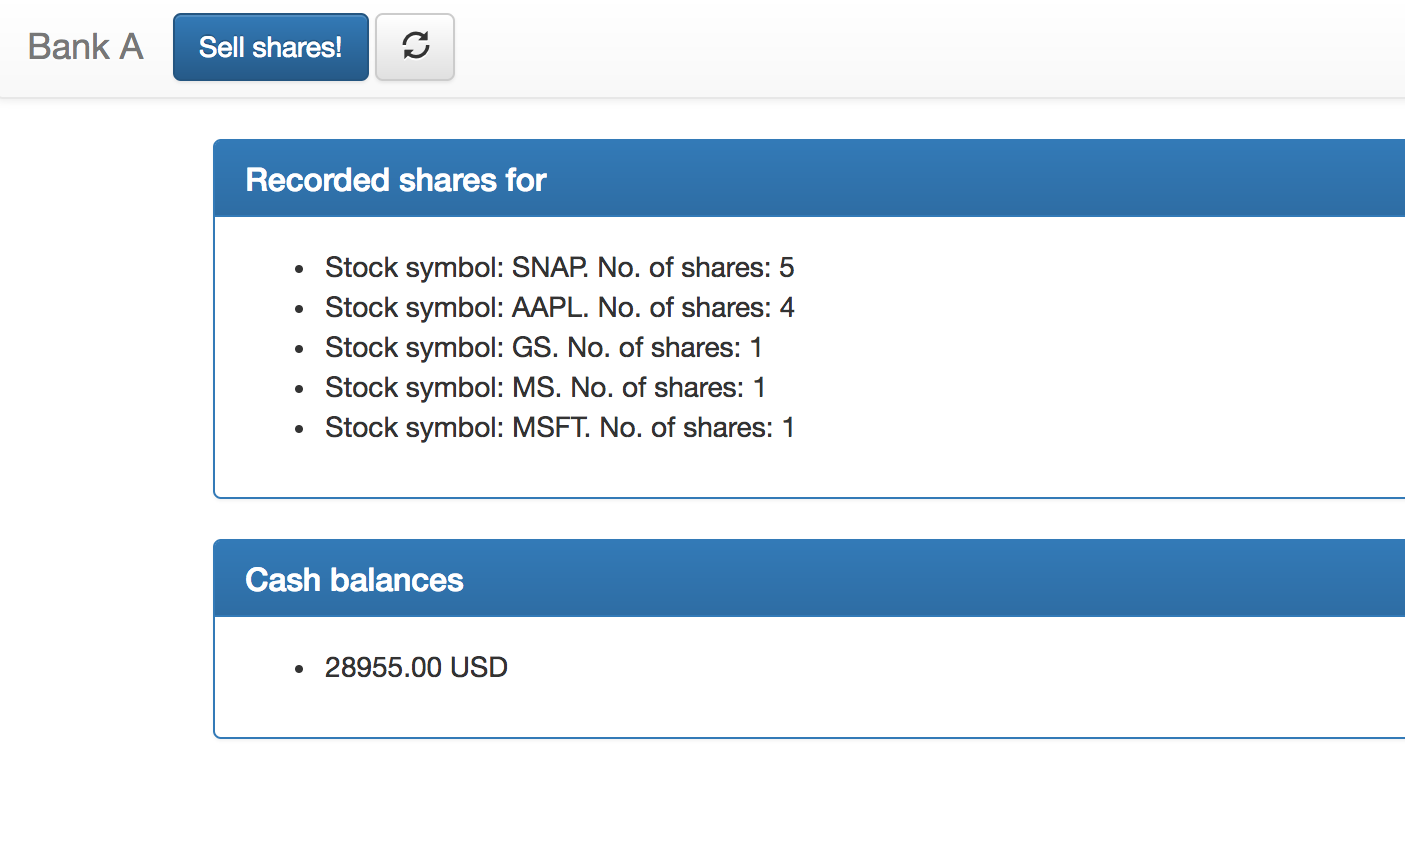
\includegraphics[width=0.85\textwidth]{node.png}
        \caption{Bank A's web interface}
        \label{fig:node}
    \end{subfigure}
    ~
    \begin{subfigure}[b]{0.85\textwidth}
    	\centering
        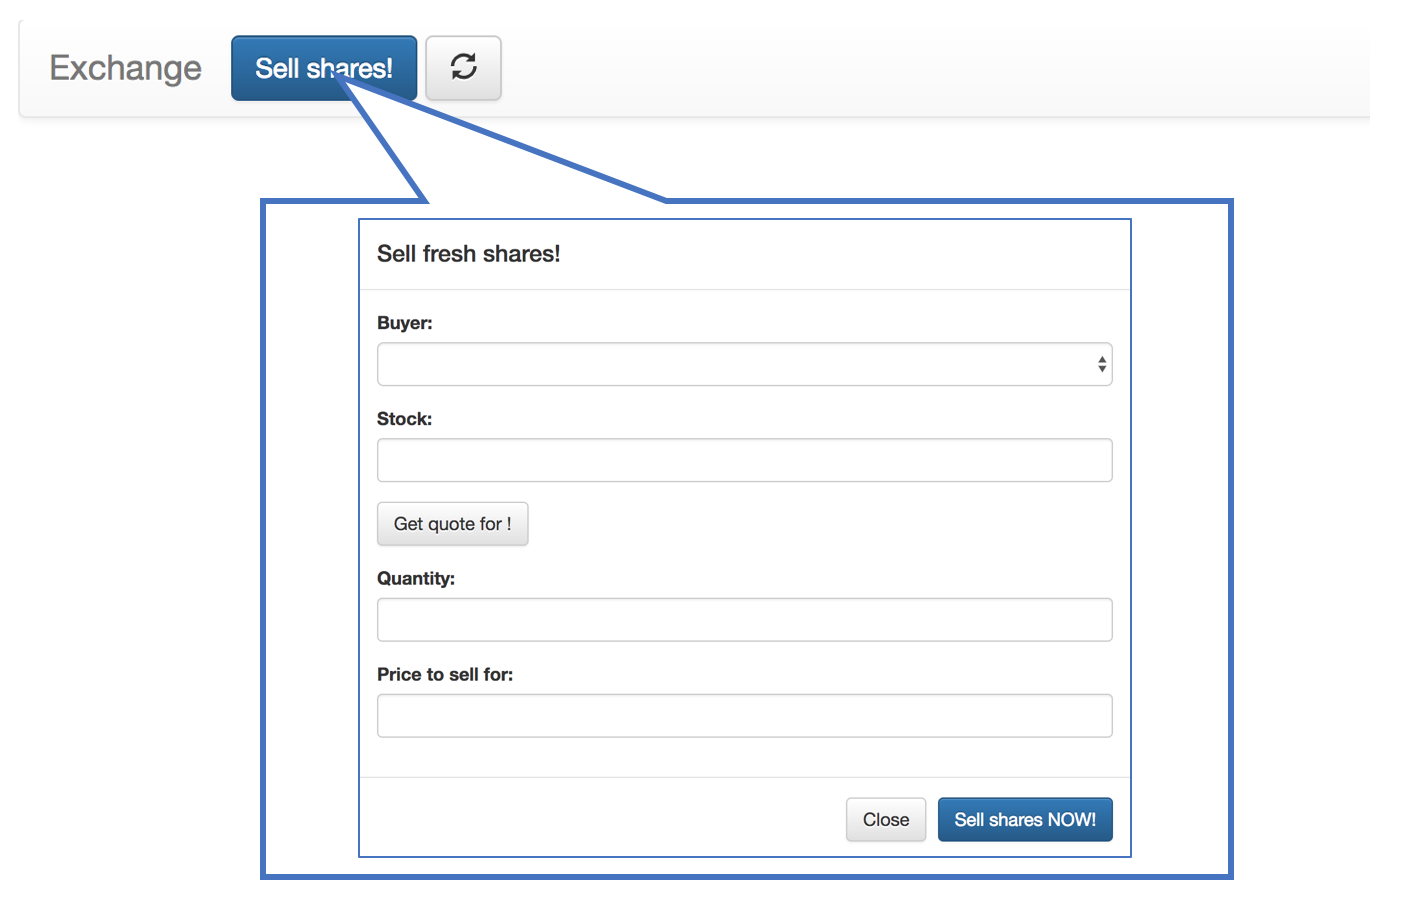
\includegraphics[width=1\textwidth]{exch.png}
        \caption{The exchange's basic web interface}
        \label{fig:exch}
    \end{subfigure}
    \caption{Vault contents, including already used states}
    \label{fig:WEBinterfaces}
\end{figure}
\\ \\
In the angularJS module, we have several modals that deal with different parts of the web page. The main controller (\verb|DemoAppController|) calls most of the GET methods to determine the current node's identity, its peers and its cash and share balances. The \verb|ModalInstanceCtrl| deals with the the menu that opens up when we decide on selling shares - it can create a trade between itself and a counterparty and it can get real-time quotes from Yahoo! Finance. It also validates any purchase order, according to the rules set out before (no negative shares, just text input for freetext boxes). The final modal deals with displaying messages, which happen after a transaction is triggered - either a confirmation that it was committed to the ledger or a detailed error explaining why it could not be finalised.
\\ \\
Although the web pages are currently in a very basic format, they are meant to demonstrate the fact that the applications can be really easy to use, without requiring any previous programming knowledge. The structure is similar to the one used in other demos, giving a unifying theme throughout. From a security point of view, the current demos do not work on HTTPS and are not using certificates. However, a discussion about these points can be found in Section \ref{sub:Security}.
\newpage
\section{Applications}
\label{sub:apps}
After the presentation of each building block altered or created for the purpose of this thesis, we will now present the applications that bind all of these together. Their goal was to showcase specific features of the system and prove that having Corda as a codebase is both achievable and worthwhile. First of all, we will present a distributed system that has accessible web interfaces for every participant. This will demonstrate that trading can be easily done in our project, taking only a few seconds to reach consensus between parties, clear the trade and settle the transaction (as opposed to the current three-day standard). Secondly, we will look at the scalability of the system from the point of view of transactions: can we emulate a real-life market along with its random variables? Lastly, we will look at scalability from the point of view of participants as well: what happens when we want to expand our consortium of banks? 
\\ \\
These applications are presented in depth from a technological point of view in this section. However, given that some of them present some restrictions and limitations, we will re-visit them in the Evaluation Section (Section \ref{sec:Evaluation}). There, we will look at node configurations, network restrictions and performance metrics.
\\ \\
As a preamble to the description of each application, we will first explain their structure. This is also explained in the User Guide (\ref{sec:UG}), detailing how one could potentially deploy, start and use the nodes. Given our Corda implementation, we have a gradle task that can be triggered to deploy the nodes. This creates a folder with a number of nodes, each having their own permissions, configurations and port numbers. While this process is done locally, we do not want to stop here, because the nodes are meant to be working from different machines, with different IPs. At this point, we move the deployed nodes to the desired machines (with \verb|scp| or the help of a flash drive) and replace the IP with the correct one. Note that this step is only required to be performed \textbf{once}.
\\ \\
Starting the nodes means that each node's execution is performed in a separate terminal. On a Mac, there is no support for X11 anymore so throughout the thesis the examples are using XQuartz. This only affects the graphical interface of the terminal windows, not the performance. Once the nodes are registered with the network controller and connect to their database servers, they are ready for usage. At this point, we can choose to execute flows from within the nodes' dashboards or from a main controller (using gradle tasks).
\subsection{The \textit{Distributed web system}}
\label{sub:sharedEX}
The first application was created to demonstrate the ease of use of the system. We chose two virtual machines to distribute our eight nodes to. To expand the network either by adding more machines or more nodes, the only modification is in the node configurations of the new nodes - they have to have the IP of the network controller. In this case, the notary acts as a network controller as well, having the information about all the nodes on the network. Among the nodes, we have Bank of Corda (a cash issuer meant to emulate a Central Bank), the Exchange (a share issuer creating new shares; mock facility to populate the vaults of the network participants) and the other five banks which perform trades among themselves.
\\ \\
\begin{figure}[!htb]
\centering
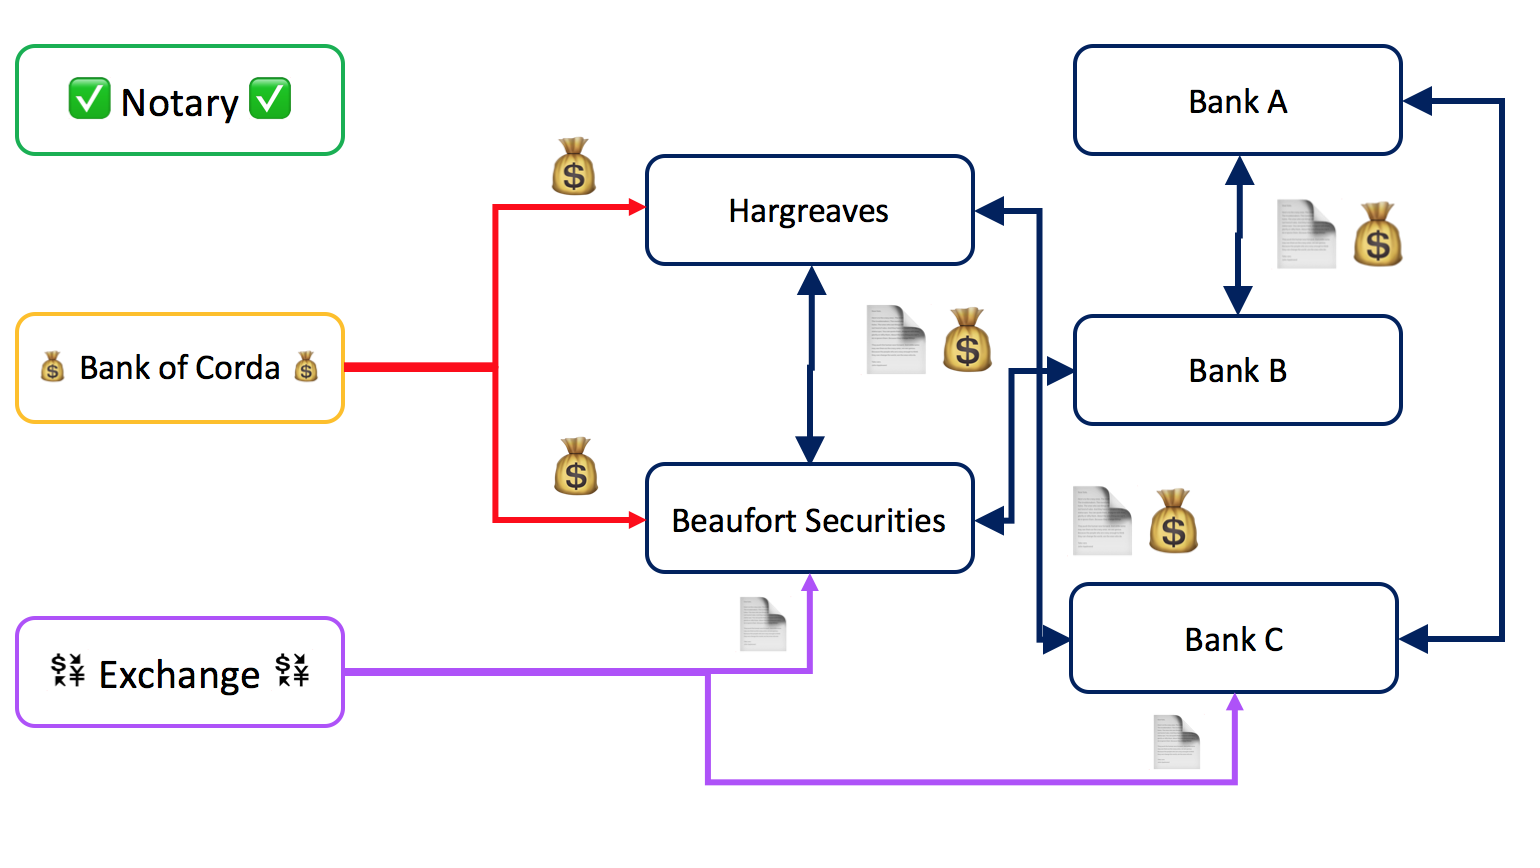
\includegraphics[width=1\textwidth]{archdiagramSHEX.png}
\caption{Architecture of the application}
\centering
\label{fig:shEx}
\end{figure}
\\ \\
All of the banks and the exchange have a dedicated web server, used to serve the graphical interface. Commands can be executed via the terminal of one of the VMs, as well. The only command that is pre-executed (it cannot be executed on the website) is the cash issuance. This is purely done as a safety measure since we wanted to recreate a real-world example, where banks cannot request money continuously. 
\\
\begin{figure}[!htb]
\centering
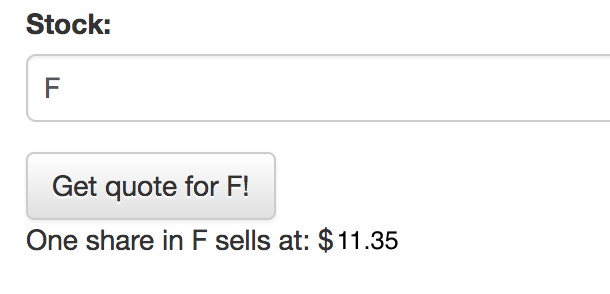
\includegraphics[width=0.55\textwidth]{quote.png}
\caption{Real-time quote for stock F}
\centering
\label{fig:quote}
\end{figure}
\\
A graphical description of the application's architecture is shown in Figure \ref{fig:shEx}. As it can be seen, the Exchange is the only one permitted to perform the \verb|SellerFlow| (the purple lines), while the banks can all perform \verb|SellerTransferFlows| among each other (the black double-ended lines). Bank of Corda issues cash to the participants (represented by the red cash lines). To note that while only a few connections are shown on the architectural diagram, this was done solely for the purpose of having a clear image - Bank of Corda \textit{can} issue cash to all of the banks (all the black-box participants) and the Exchange \textit{can} sell fresh shares to all the banks, too!
\\ \\
To give a sense of what the application is able to do, we provide an example run. Suppose that Bank C wants to buy 10 shares in Ford Motor Industries (F) at the price offered in the exchange. As mentioned before, we have to activate the transaction from the seller's side, in this case the Exchange - this action would be performed by a broker. When we input the parameters of the trade that we want to perform, we can also check the real-time price of a share in F by clicking the \verb|Get Quote!| button (Figure \ref{fig:quote}). \\ \\
\begin{figure}[!htb]
\centering
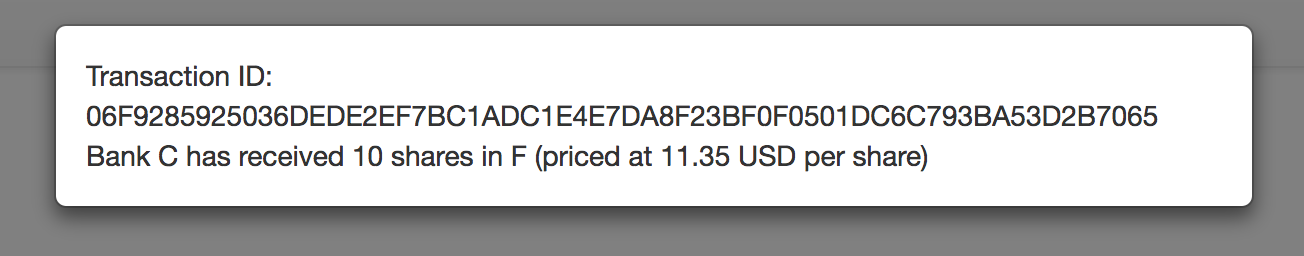
\includegraphics[width=1\textwidth]{conf1.png}
\caption{Confirmation of fresh shares generation and sale}
\centering
\label{fig:conf1}
\end{figure}
\\
\begin{figure}[!htb]
\centering
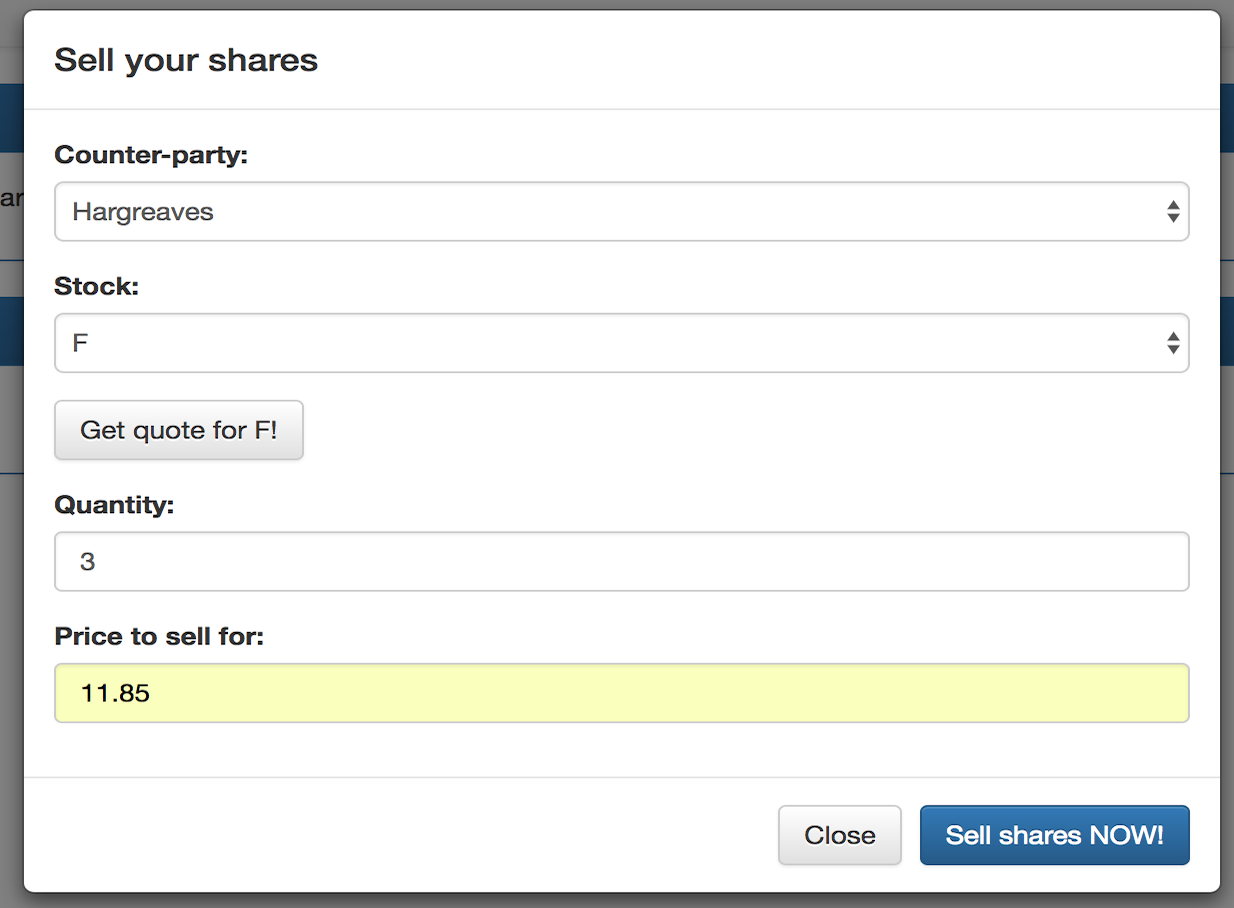
\includegraphics[width=0.65\textwidth]{shareSale.png}
\caption{Share sale menu in one of the market participants}
\centering
\label{fig:shareSale}
\end{figure}
\\
After submitting the transaction for processing, we get a confirmation like the one in Figure \ref{fig:conf1}. Behind the scenes, a \verb|SellerFlow| creates a new ShareContract, changes its ownership to Bank C and a delivery-vs-payment process takes place. We can now refresh our vault view in Bank C's site and move on to the next operation.
\\ \\
We have some shares and we have some cash in our vault, but now we want to trade some of those shares. Suppose there is an external broker request for a trade of 3 Ford shares from Hargreaves. In Bank C's share sale menu, we input the details of this transaction (Figure \ref{fig:shareSale}). For this operation, internally a \verb|SellerTransferFlow| is triggered, performing an asset swap by using existing shares from the vault as opposed to creating new ones, like in the Exchange's case.
\\ \\
Again, for this we get a confirmation or a failure notice. The confirmation takes a a different form, showing the transaction ID of both the cash and the share state (Figure \ref{fig:conf3}). 
\begin{figure}[!htb]
\centering
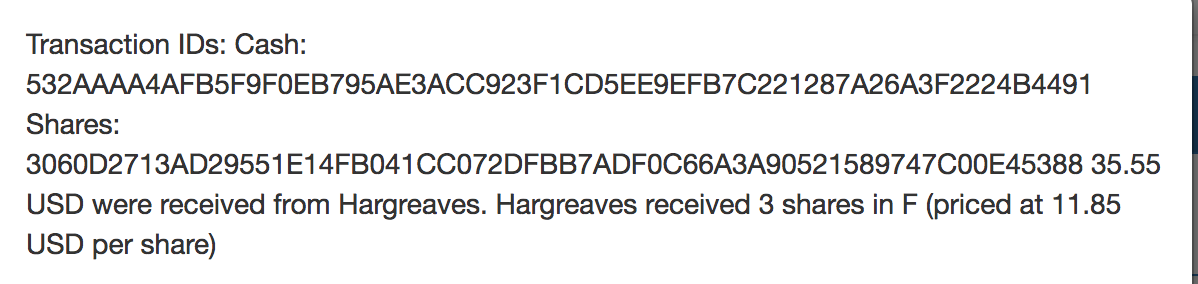
\includegraphics[width=1\textwidth]{conf3.png}
\caption{Confirmation of successful share transfer (with cash and share transaction ID reporting)}
\centering
\label{fig:conf3}
\end{figure}
\\ \\
However, if the price we set for our transaction is inappropriate or we do not have enough assets in our vault, we receive a failure notice (Figure \ref{fig:conf2} and Figure \ref{fig:conf4}).
\begin{figure}[!htb]
\centering
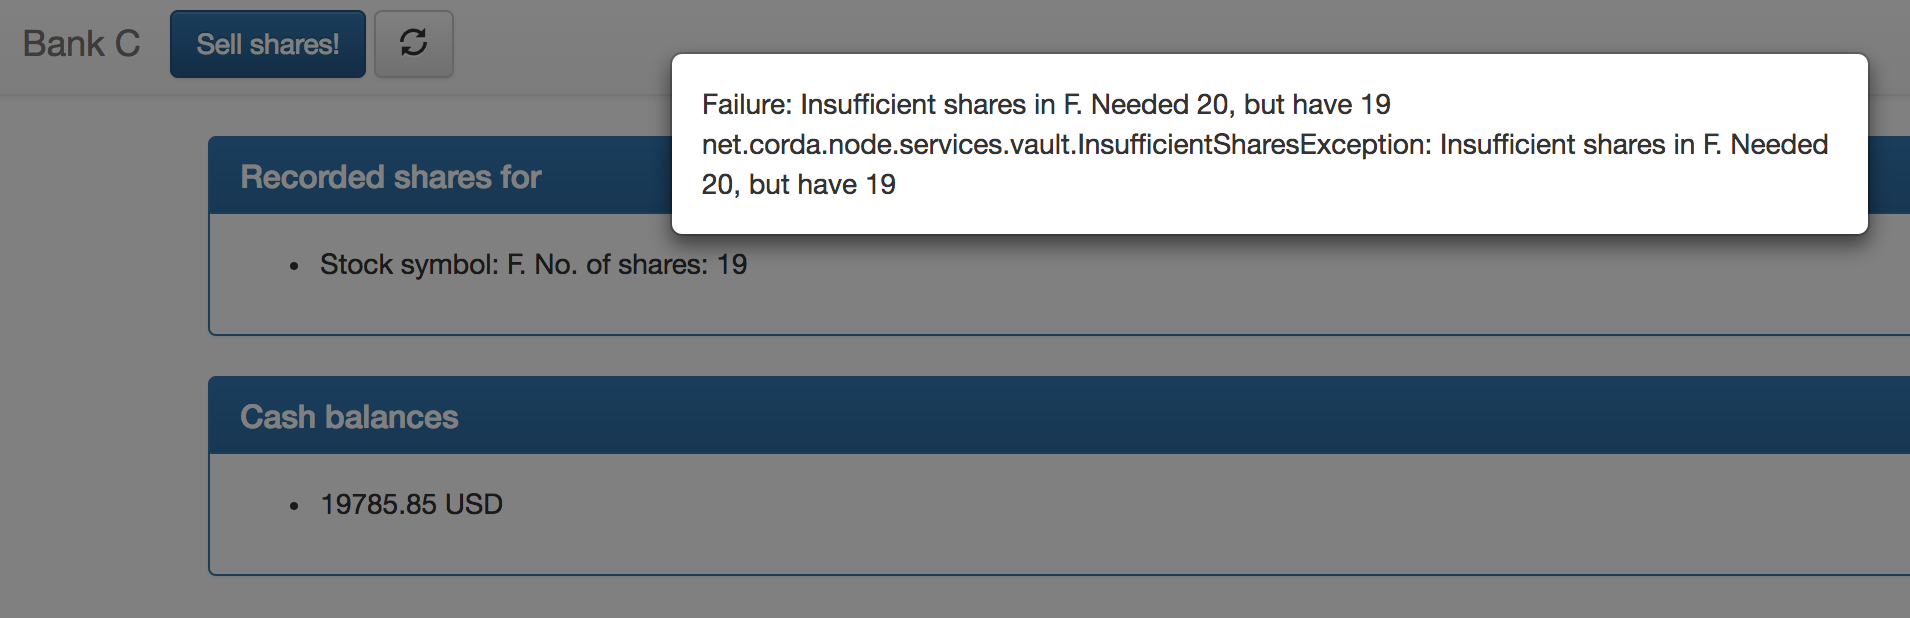
\includegraphics[width=1\textwidth]{conf2.png}
\caption{Failure notice due to insufficient assets in seller}
\centering
\label{fig:conf2}
\end{figure}
\\ 
\begin{figure}[!htb]
\centering
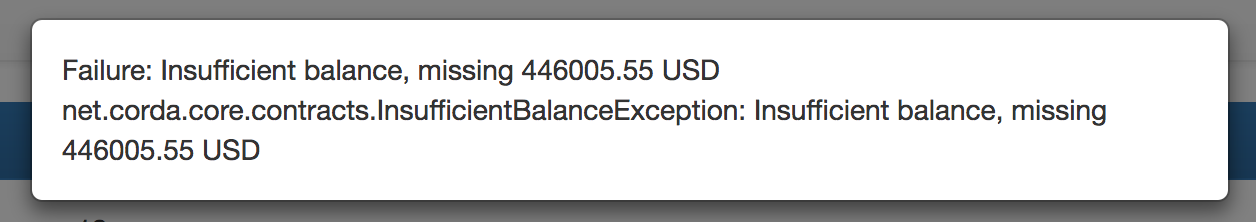
\includegraphics[width=1\textwidth]{conf4.png}
\caption{Failure notice due to insufficient funds in buyer}
\centering
\label{fig:conf4}
\end{figure}

\subsection{The \textit{Random distributed marketplace}}
\label{sub:mkt}
If the previous application shows that share contracts can now be traded between market participants in a matter of seconds, this application goes one step further. A marketplace has a plethora of random variables and trades occur very fast, very often! To simulate such an environment, we decided to create an application that will just perform random trades between random participants. This means that we randomly pick a stock and we attempt to sell it to someone in the market. There are a few things that can happen and we need to be guarded against them - we might not have the stock in our vault or the buyer might not have enough money. Although the application is relatively primitive, it fulfills its goal of proving the scalability of the system. Transactions are not being delayed just because all the market participants are trading almost at the same time - the explanation for this is provided in Section \ref{sub:Performance}.
\\ \\
\begin{figure}[!htb]
\centering
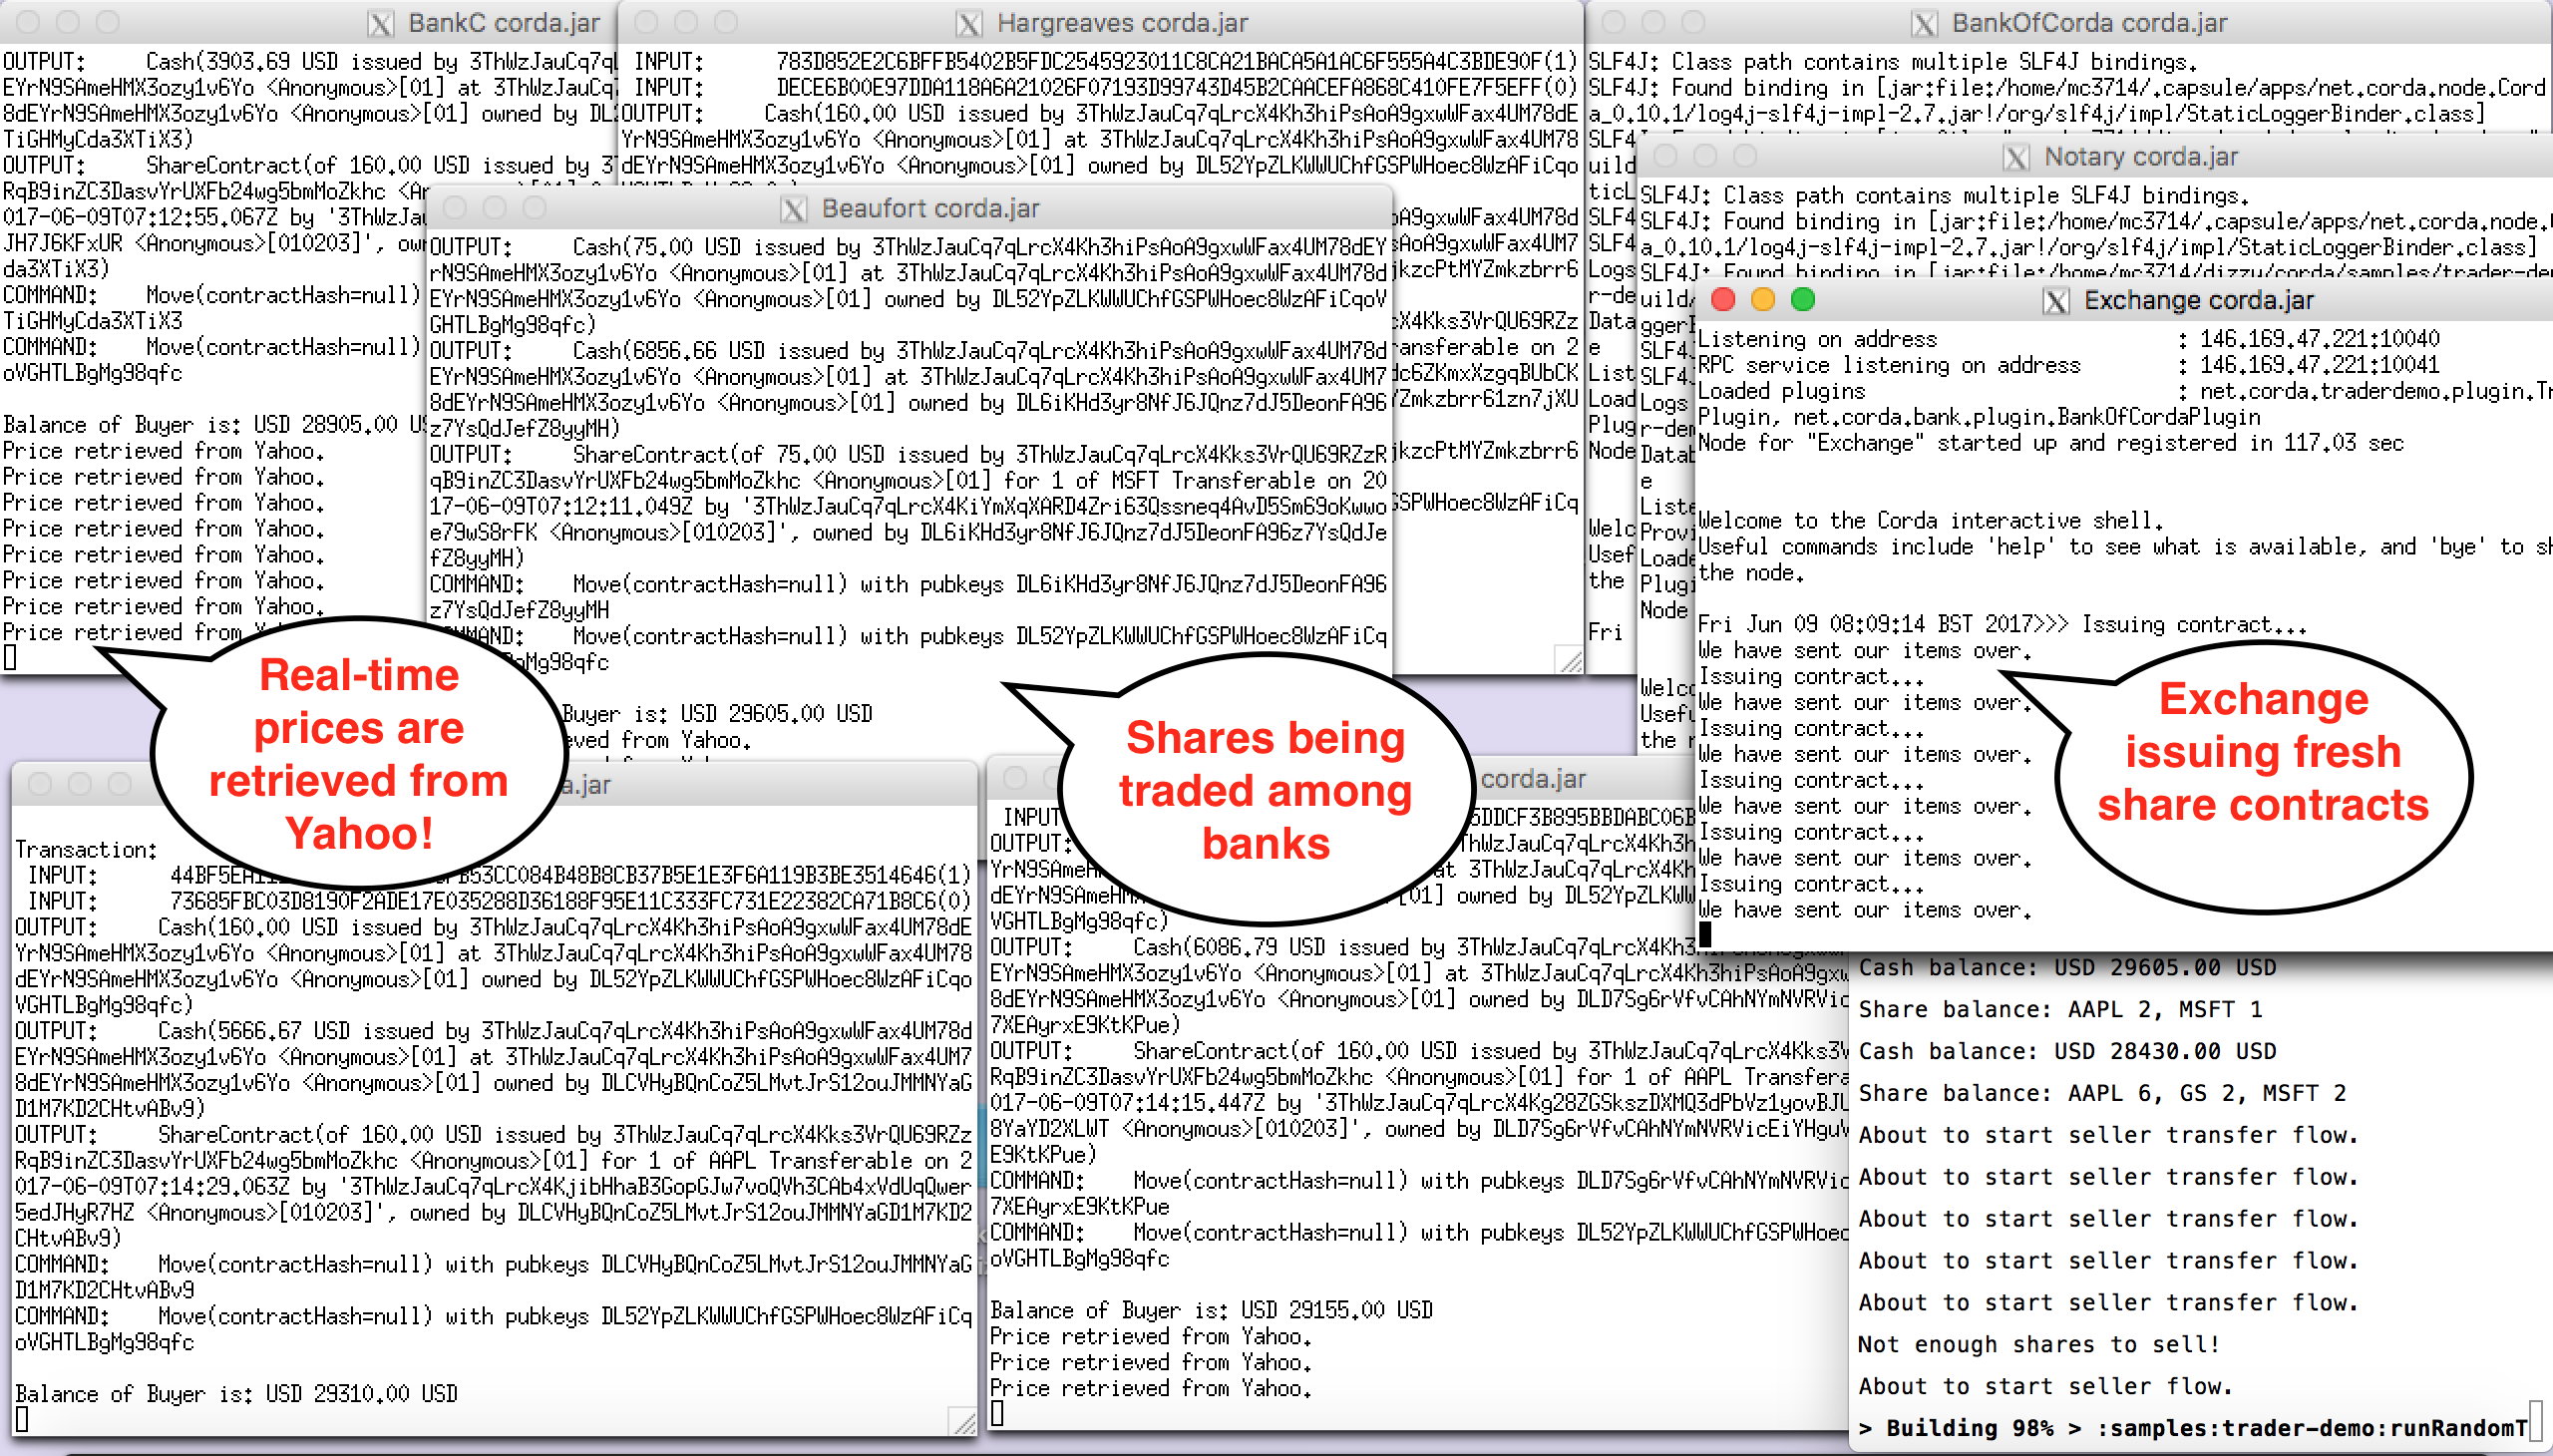
\includegraphics[width=1\textwidth]{random.png}
\caption{The random distributed system}
\centering
\label{fig:random}
\end{figure}
\\ \\
The architecture of the system is similar to the one in the previous application. The main difference is that there is no input from a ``broker" in this case since everything is done automatically. A snapshot of what the system looks like in the middle of trading can be seen in Figure \ref{fig:random}.
\\ \\
To assess the state of the ledger from time to time, there is a call to query the vaults of the participants once every twenty transactions. This way, we can ensure that trades are indeed taking place correctly and assets are being exchanged between the participants. An example of this can be seen in Figure \ref{fig:balances}, which details the vaults of each participant, in order (starting with Bank A and ending with Hargreaves).
\\ 
\begin{figure}[!htb]
\centering
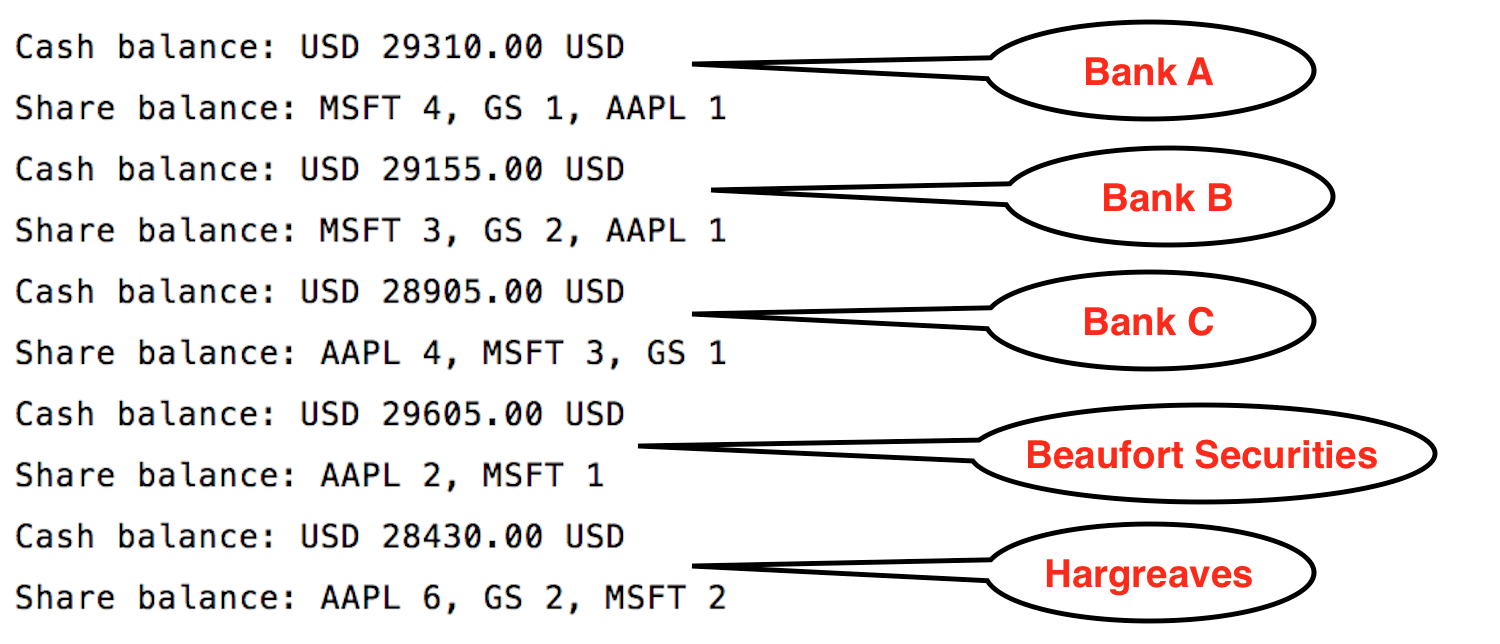
\includegraphics[width=1\textwidth]{balances.png}
\caption{Balances of the five market participants}
\centering
\label{fig:balances}
\end{figure}
\\ \\
An improvement this application could have is to implement a multi-threaded trade system. While currently the transactions are being created and performed sequentially, within one banking consortium, we could expand this further. Having a transaction-per-thread system would increase even further the number of transactions that can be performed by the market participants. Moreover, now there are four nodes per machine. Ideally, the nodes from the real-world system would have a dedicated machine to run on, so there would be even more possibilities of performing trades.
\\ \\
The bottleneck would shift to the notary node, which would still have to deal with all transactions in the system. This problem can be solved either by introducing a notary group (multiple notary nodes, each being able to validate transactions in parallel) or by splitting the system into two groups, each with their own notary. While this application helped discover more about the performance and scalability potential of the system from a practical point of view, there is also a more theoretical approach to these matters in Section \ref{sub:Performance}.

\subsection{The \textit{on-the-fly node addition}}
\label{sub:flynode}
Scalability can also be assessed from the point of view of system contributors. How many banks can we have in the system? Does their addition influence performance? This part discusses the ways that nodes can be introduced into the system, determining an optimal solution for this task.
\\ \\
\textit{Changing the build script:} Since nodes and their configurations are defined in the build.gradle file, an idea would be to change the task deploying the nodes by adding a new one (Listing \ref{l:nodebad}). This is cumbersome, includes modifying actual source code and does not represent good software practice. This method was used during development to test whether node addition had an influence on existent nodes. We found out that the existent nodes are not affected by the deployment changes, but they do have to be stopped and started again if we want them to recognise the newly deployed node.
\\ \\
\textit{Copying a fresh node instance:} After the initial deployment, nodes have a basic structure: the configuration file, the corda.jar which contains the binaries used by the system and the libraries needed for correct functioning. If we wanted to add a new node, we could duplicate one of these nodes (the folder) and change its configuration by modifying the node's parameters (port numbers, name, location, permissions). Once the nodes are started up for the first time, they connect to the network controller and set up their certificates. Again, for this to take effect in the new node, we would have to stop the running ones and restart them after we copy the new node's folder. While this is the method the Corda developers are currently using to deploy new nodes, this project wanted to take things a step further and aim for no node restarting.
\\ \\
\textit{On-the-fly deployment:} The goal was to deploy a new node while all the existing nodes were still running, to mimic a scenario that would happen in real-life. To maintain a performant system, you should not be required to stop everything just to add a new participant. Therefore, this solution deals with the restarting issue by using a separate gradle task meant to add a new node (to the same node group) that is related to the same notary and cash issuer as the others (Listing \ref{l:nodegood}). The deployment is similar to the previous two solutions - a new folder is created, but this time, there is no need to change the configurations since these are being fed into the node folder from the gradle task. The remaining step is to start the node (and optionally, its web server) and this is achieved by calling a small script which runs the newly deployed node. Whenever we perform an operation from one of the market participants, we will see the newly added node as a peer on the network and we will be able to trade with it. Therefore, this is the optimal solution for adding new nodes to the consortium. 

\newpage
\section{Evaluation}
\label{sec:Evaluation}

\subsection{Nodes}
\label{sub:Nodes}
\subsubsection{Network}
The most important feature in a distributed ledger is the possibility of spreading out the nodes on different machines, in different subnets, in different regions. The demo applications developed by Corda's creators (especially their commercial paper trading demo) have been built so they can run on only one machine. However, we wanted to have more flexibility in terms of where the nodes are being hosted. Therefore, the first step was to distribute the nodes on virtual machines. However, this functionality is currently not automated. The node configurations can be accessed and modified, but this process is manual for the time being. The configuration of a node specifies its name and location, the network map service controller it belongs to, its ports and its permissions. We have the RPC and P2P ports used for inter-node communications and optionally, a web port in case the node has a web site attached. The permissions represent the users that can access the node and, for each of them, the list of flows they are able to call. An example of a configuration file can be found in the Appendix.
\\ \\
At this point, connections can be established \textbf{only} if the machines are on the same subnet. This behaviour can be seen in the following figure, with the 3 nodes being run on 2 Azure VMs (Controller, Bank B and Bank C are on machine1 and Bank A is on machine2, having different IPs, but on the same subnet). However, no trade is able to take place between the 2 machines in their demo because of insufficient configurations. \\ \\
\begin{figure}[H]
\centering
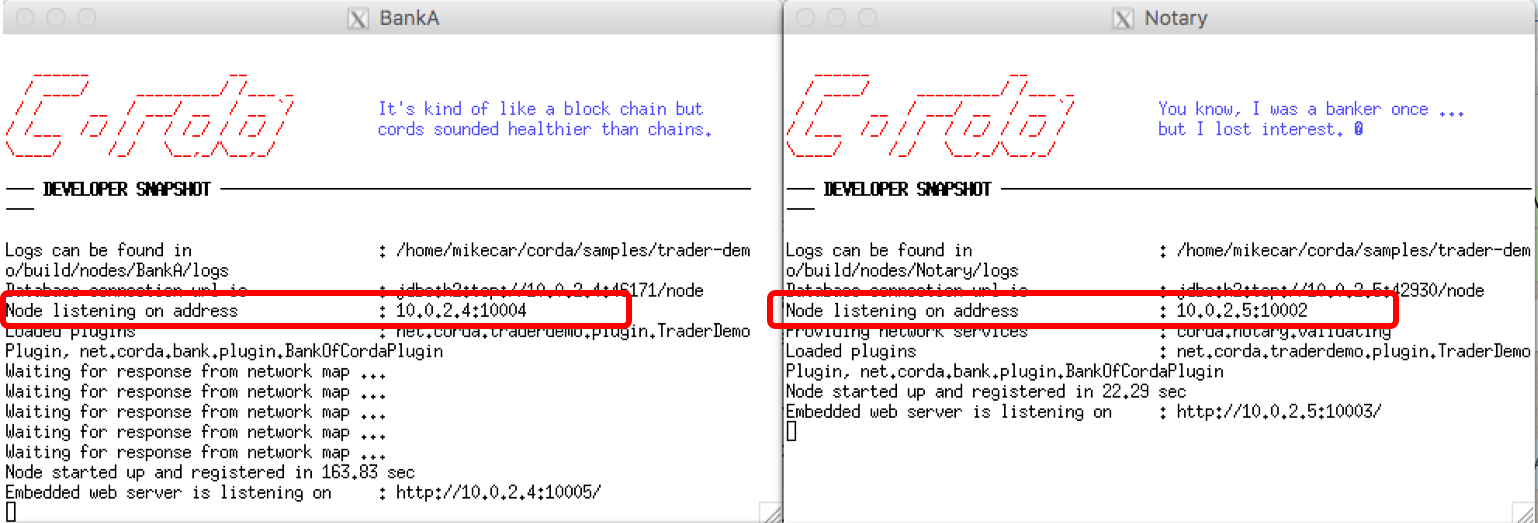
\includegraphics[width=1\textwidth]{diffips.png}
\caption{Distribution of nodes on 2 machines (different IPs)}
\centering
\label{fig:IPs}
\end{figure}
For the applications developed, we ensured that the configurations of the nodes allow them to both be spread out on several machines and be able to perform operations from them. An attempt to move nodes on machines that are not on the same subnet has been made as well, but this is a behaviour that is planned for future implementation by the developers. Even so, for the moment, we can consider that we have a subnet dedicated to the banking consortium. To be able to achieve a uniform performance throughout, the network participants should have the same network characteristics in terms of speed and bandwidth.
\subsubsection{Nodes and vaults}
\label{vaultnode}
The current node infrastructure is still in development. Because of this reason, currently there can only be one vault attached to one node. This means that, if we represent a bank with a node, then a bank can only have one customer. Of course, this is not the case in the real-world so we have to find a way to work around this. Although the final version of the Corda project does plan on having multiple vaults per node, for the moment, this thesis worked under the assumption that we can only have one customer for each node.
\\ \\
\begin{figure}[!htb]
\centering
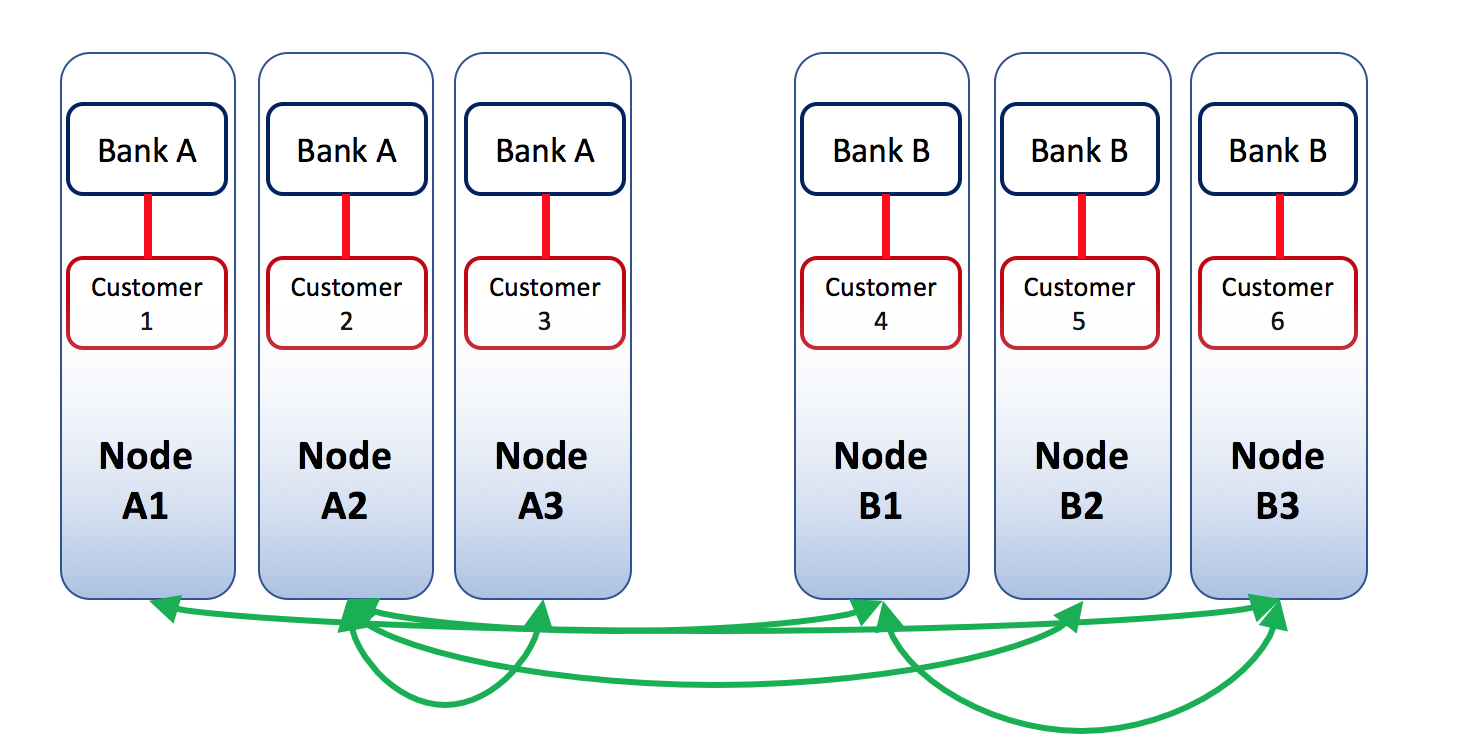
\includegraphics[width=1\textwidth]{bank1.png}
\caption{One node per customer}
\centering
\label{fig:bank1}
\end{figure}
\\ \\
This leads to a few points that have to be settled in this scenario. Since a bank has more than one customer, how can we accurately represent it with nodes? One solution would be to create a node sub-group for a Bank (say, Bank A). Therefore, we would have as many nodes as Bank A has customers! While this represents the situation correctly, it does not mean that it is efficient. Each node will have to be hosted (ideally) on a separate machine and, while the opportunities for parallelism are very good in this case, there would be some resource contention and higher energy consumption. Flows would be initiated by each node (so, for each customer, the custodian or broker of that account would run the flows directly from their nodes) A diagram of what this scenario would look like is shown in Figure \ref{fig:bank1}.
\\ \\
Another option would be to have an entity that oversees and controls all the information and operations that take place within it. This router-node would act as a super-node, delegating flows to each particular node and redirecting input and output accordingly. This is presented in Figure \ref{fig:bank2}. 
\\ \\
\begin{figure}[!htb]
\centering
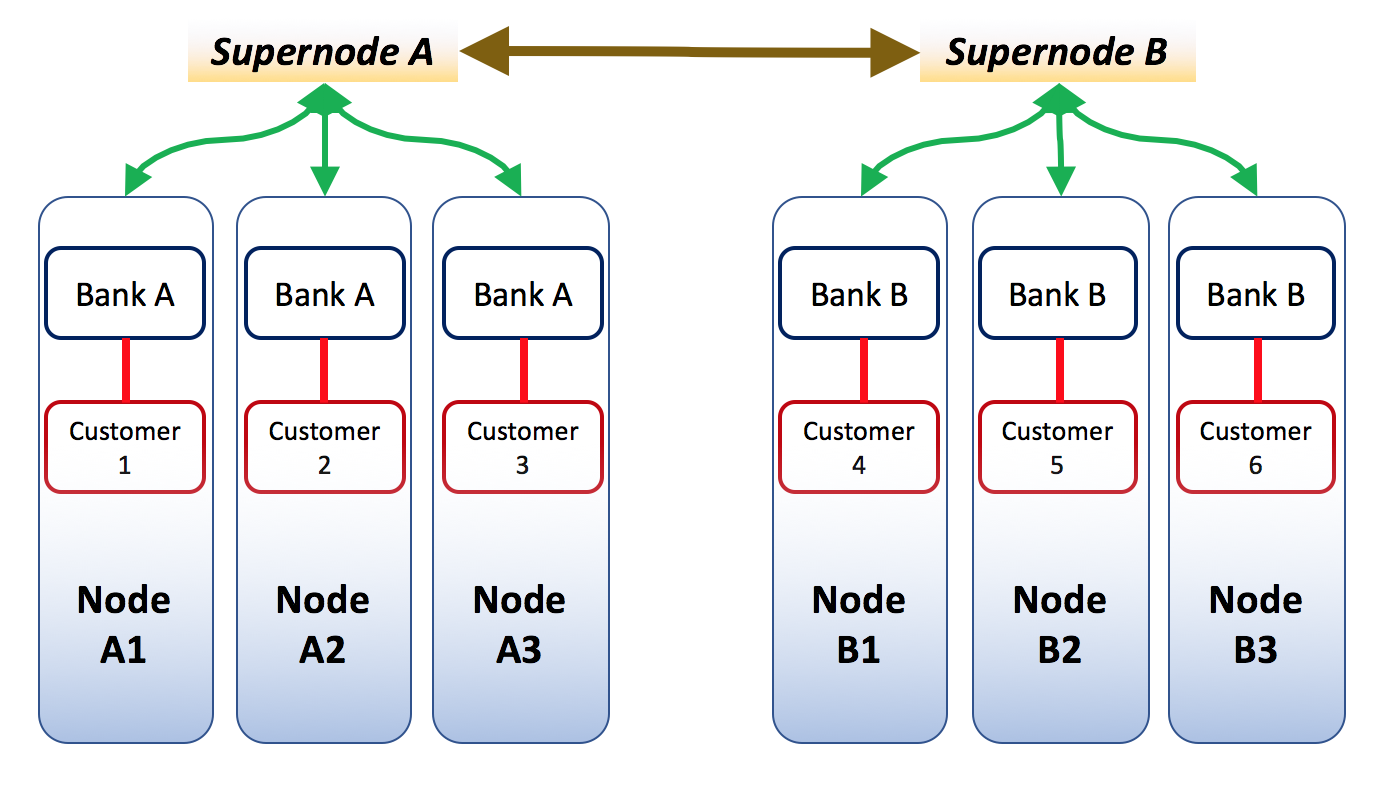
\includegraphics[width=1\textwidth]{bank2.png}
\caption{Supernodes delegate flows}
\centering
\label{fig:bank2}
\end{figure}
\\ \\
\begin{figure}[!htb]
\centering
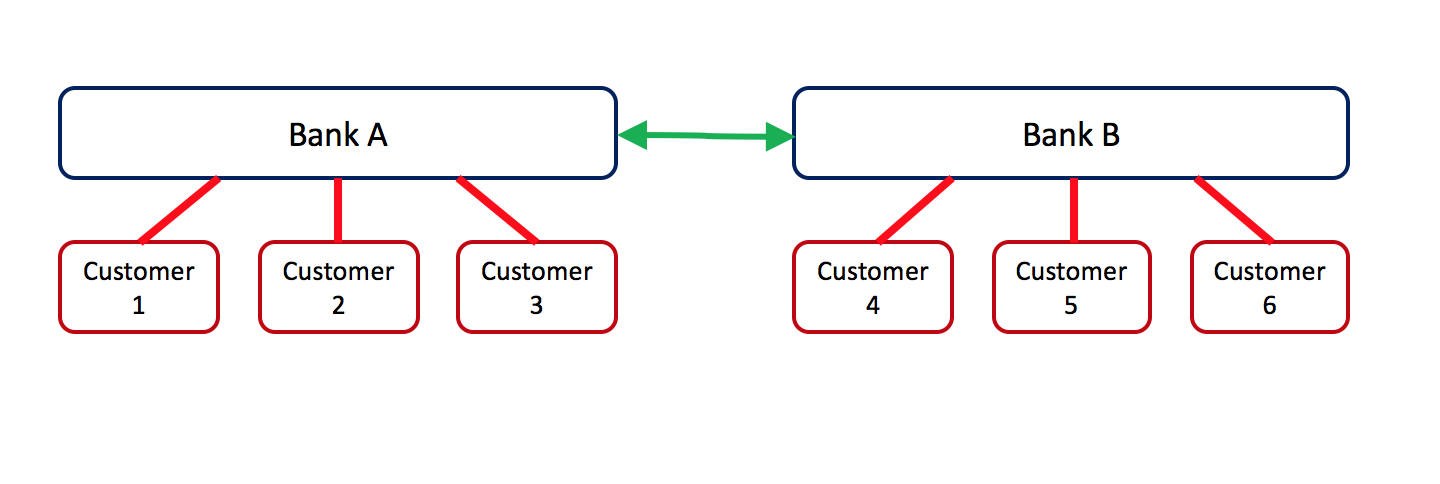
\includegraphics[width=1\textwidth]{bank3.png}
\caption{Ideal, final node to customer vault representation}
\centering
\label{fig:bank3}
\end{figure}
\\ \\
The previous solution is similar to the final version of the system, which sees the node acting as a router for all the vaults instead, emulating the current banking views. This can be seen in Figure \ref{fig:bank3}. 
\\ \\
Given that this part is still up for modification in the codebase, we have decided to use the assumption that each bank has exactly one customer (a one-to-one relation between nodes and vaults) in the applications developed. It is expected that any changes made to the node infrastructure would have a limited effect on the applications - the only major change that will need to be done is the correct redirection of funds and assets to a vault that is located \textbf{within a node}, rather than just the node itself.

\subsubsection{Zombie nodes}
\label{sub:zombies}
One issue that came up during the development of the applications was the imperfect exception handling mechanism for nodes' internal failures. Since there have been plenty of node deployments for the duration of the development, some of them were triggered without ensuring that all the previously running processes have been shut down correctly. This sometimes led to node fragments (configurations, open ports, blocked resources) being left uncleaned. The applications do not support dynamic port changing (at least for the time being), which meant that when they were re-deployed, they would not behave normally. Bad behaviour included nodes being unable to fully start up, unable to register with the network map controller or unable to perform connections with other participants.
\\ \\
Another problem that generated ``zombie nodes" was bad database accesses. If a flow contained an error related to suspendability or serialisation, the node would fail and affect the database. This database corruption would stop the node from being restarted correctly. A full clean-up was necessary to remove any node fragments, as well as checking whether any processes were left running (and killing any of those).
\\ \\
This fragility is constantly being dealt with in the newer releases of Corda: serialisation problems for starting flows are fixed in version M11.1 and Artemis connection problems are being worked on for an upcoming release. However, this prompted the need for contract and flow tests, verifying their behaviour in a confined environment. 
\subsection{Flows}
\label{sub:Flows}
As discussed in the previous section, problems introduced by bad flow terminations had to be limited as much as possible. An integration test facility was created to ensure all the flows behave correctly, without posing any operation threat during their execution within an application. For this to be productive, there is a dynamic port numbering (new ports for every run), as well as using a lighter version of the nodes which enables faster testing. This also enabled us to test the auditor feature in an easier way.
\\
The integration tests are also used to prove permissioning facilities. We register different sets of flows to different nodes and we prove how an unauthorised user cannot have access to a node's internal system or, how a node that does not pre-register a flow is not allowed to use it. This related to the way Bank of Corda and the Exchange have a protected usage characteristic - for example, the Exchange is the only one allowed to run the \verb|SellerFlow| which generates new shares.
\subsection{Cash and asset issuers}
\label{sub:cashissuers}
This project discussed money at length. We used ``cash" to perform trades, but what exactly is this cash, how did it get there and what is its value? Well, in the real world, cash - the coins and notes we are so used to now - is actually worthless. There's just pieces of metal or paper, without any real value. However, since they were released by a Central Bank, they represent an obligation of payment for the user. This means that cash is actually a form of an IOU (``I owe you") - a deposit is a bank's obligation to convert the physical money into currency (that you can put into your account, for example).
\\ \\
As shown in Section \ref{sub:DistributedLedgers}, most available blockchain systems use their own form of cryptocurrency to avoid interacting with Central Banks for money issuing. Although initially it was conceived with the goal of interchanging money anonymously, this soon became a problem with illegal trades being performed on the Dark Web. It was discovered that anyone can track the transactions performed anyway, so the traceability of transactions (and, inherently, of money) could easily be done. However, newer systems (compatible with Bitcoin) attempt to make it harder for people to track the transactions by de-anonymising users. This would enable people to use bitcoins for money laundering or illegal trades and then bring the bitcoin back onto the public market for trades made by law-abiding users. This makes it a problem for our system and we desire both a direct interaction with Central Banks for digital money reflecting existing fiat currencies and a way to have the currency's provenance easily analysed \cite{tumblebit}.
\\ \\
Another problem with using cryptocurrencies is that they are quite volatile. Bitcoin first traded for roughly one tenth of a cent per bitcoin, in 2009 \cite{first}. That price increased slowly over time, however, in May 2017, its price more than doubled. Although Bitcoin is nowhere near mainstream usage or acceptance, the surge in price could be an effect of increasing demand for the currency in markets like the Asian ones \cite{voxbubble}. Many critics say that the recent price changes are signs of a bubble, because ``ascents this steep are rarely unsustainable" \cite{bubble}. This hints at even more volatility along the way as opposed to the solution Central Banks would turn to when trying to digitalise their monetary systems. Even more, as mentioned previously, the cryptocurrency market would have to be highly regulated before mainstream use and definitely extensive controls would have to be put in place to enable them to be used in the financial world.
\\ \\
Therefore, Corda and this project argue that to move the current banking system to an improved version, we need to introduce Central Banks as part of the system without relying on cryptocurrencies (although they could be traded on the system, as well). Besides the legal issues it would solve, digital cash would bring plenty other advantages as well: it widens the range of options for monetary policy (meeting a bank's target price of stability would be much easier, because we could just ``drop" newly created cash to all citizens), it encourages competition and innovation in the market (the regulatory framework would make it easier for the financial sector to offer different kinds of accounts) and it makes the financial system safer (by clearing in central bank money directly, instead of doing it in bank deposits, we reduce the concentration of liquidity and credit risk in the system) \cite{digcash}.
\\ \\
To implement this system, Central Banks would have to own their own nodes - in a similar fashion as the way we set up Bank of Corda. These nodes would introduce money into the system, just as they would do with fiat currencies. This differs from cryptocurrencies because this money would actually be legal tender according to the government. The good news is that Central Banks are preparing for this change - they are getting ready to listen to the demand of the industry calling for newer systems using innovative technology. 
\\
\begin{figure}[!htb]
\centering
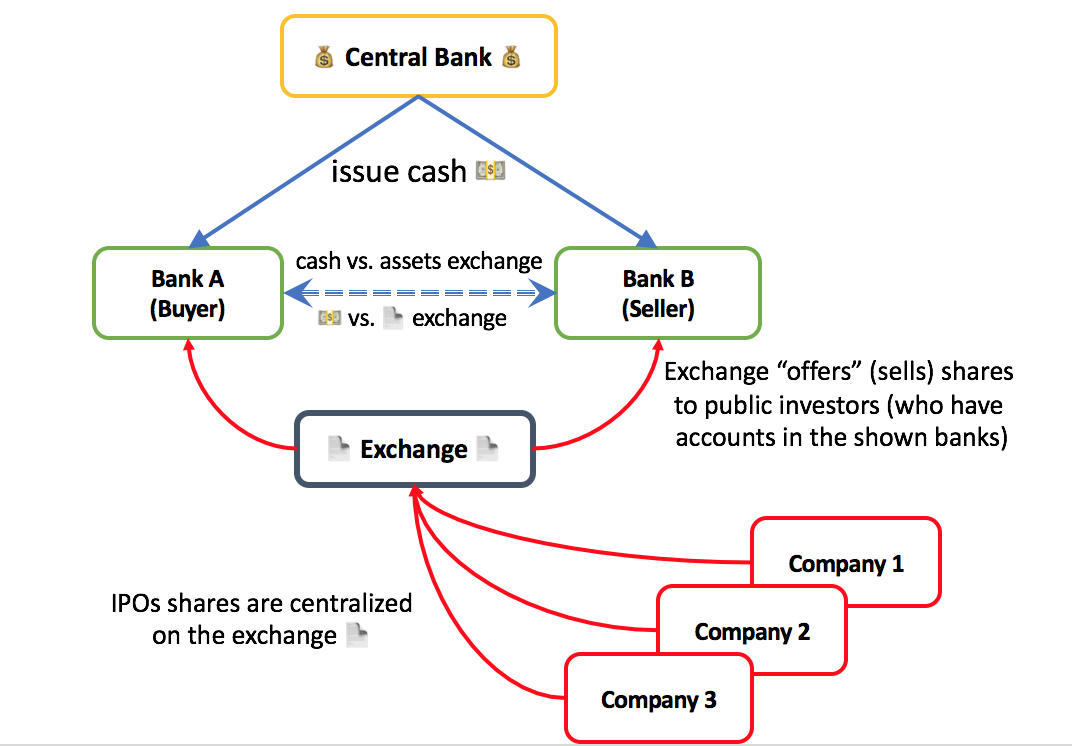
\includegraphics[width=1\textwidth]{issuers.png}
\caption{Issuing cash and assets in our system}
\centering
\label{fig:issuers}
\end{figure}
\\ \\
As an example, Bank of England's governor emphasised that they are looking into proof of concepts regarding the security of distributed ledger technologies and will expand the bank's systems to allow for DLT integration. Moreover, he recognised the advantages this would have on the accuracy, efficiency and security of wholesale payments, clearing and settlement \cite{markc}. Along with him, other central banks around the world are seeking similar goals (counting amongst them Bank of Japan, Bank of Korea and the Reserve Bank of Australia \cite{centralbanks}. 
\\ \\
A similar problem arises with the introduction of some assets to the market and their representation. There are a limited number of shares in a company, and they have been open for trading to the public market at an IPO (initial public offering - when the shares are sold for the first time). Arguably, this would be similar to the way we developed the Exchange node. We could have multiple nodes that act as entities dealing with companies' IPOs by creating the shares and selling them for the first time to one of the market participants. A diagram of how the system behaves with these components is shown in Figure \ref{fig:issuers}.
\\ \\
The provenance chain of these shares is easily explorable, with the possibility of analysing the transaction graph and finding details about the initial transaction. For example, in our project, the initial sale attaches a paper (eventually meant as a legal document of some sort) to the transaction. This can be retrieved from shares performed later on by crossing the transaction graph and looking for the issuing command. An example of this can be observed in Listing \ref{l:TG}. 
\lstinputlisting[label = {l:TG}, language=Octave, caption = Transaction Graph Search snippet]{/Users/mikecar/Desktop/Blockchain-dizzy/imgs/issuance.m}
\subsection{Performance}
\label{sub:Performance}
After thorough usage of the Corda system, it is clear that it is using an industry-standard technology stack. We see the support for messaging queues, with Apache Artemis Broker being included (but having the possibility of using any other AMPQ). This provides features such as journaling, load balancing, flow control and automatically retries to send messages (using a backoff strategy). There is a relational database with a JDBC interface - currently the database provider is H2, but there are plans of making this a flexible choice for people to be able to choose their own desired database provider.
\subsubsection{Nodes}
The performance of nodes is an important criterion to establish the overall performance of the system. While there are currently load testing facilities with which we can apply different strains on nodes and inspect different extreme conditions, they are only open to the internal development team of Corda. Nevertheless, we wanted to observe some node characteristics, even though under less strict (and formal) conditions. After successive testing on different machines, we established the average number of nodes that can be run on a ``classic virtual machine" is around 4-5. A ``classic machine" has a 4 GHz CPU and an 8 GB RAM and we have tried both Azure solutions and internal ones (provided by ApacheCloudstack). Having up to five nodes per machine means that we can have up to ten processes (for example, in the \textit{Distributed Web system} we have two processes per node - one for the corda binaries and one for the web server). This is not surprising given that each instance of Corda requires around 1 GHz to function correctly. Once more nodes are added, the machines either slow down (becoming unusable) or they fail to connect to each other.
\\ \\
This system deterioration is only noticed when nodes are added to \textit{the same machine}. However, if we consider the case that is more closely related to the real-world situation, we would have plenty of machines running nodes, so this would not pose any problems. Since connections are done in parallel for each transaction, the optimal performance is achieved when we have one node per machine.
\\ \\
We can choose to have node groups, grouping similar behaviour or simulating membership groups. One example of this in the final version of the project (where we have more than one vault per node) can be a group of nodes representing the same bank, distributing customers equally. Another option could be to have one bank node duplicated among many machines - although this suggestion would have to come with some infrastructure changes: for example, in the transaction committing we would employ a ``first past the post" system and the other requests would have to be declined. 
\\ \\
The same grouping of nodes can be seen in notarisation, as well. For example, if we choose our notary to be a RAFT cluster, we would have several notary nodes belonging to the same group, each of them being able to notarise a transaction (at the same time, for example). The downside of this is that the transactions have to be propagated into all the notary nodes' persistence database. More details about notaries' performance with respect to transactions can be found in Section \ref{sub:TP}.
\\ \\
Since we have node groups, it is easy to define different rules for each group. Although a group usually represents one entity, it can also be used by all the banks or companies covered under an umbrella (like Bank A and its subsidiary). A diagram for this situation is presented in Figure \ref{fig:notaries}. For example, from a notarisation point of view, we could have a \verb|SimpleNotaryService| (that does not provide any transaction verification, just commits it as is, shown in the blue lines) for the transactions that happen within one node-group if it represents an entity. This would make sense, because there is no incentive for a bank to perform a double-spend against itself. For cross-group transactions, we could provide a single or distributed notary service (like the RAFT cluster shown) that checks the entire transaction for correctness as well (the transaction is the green line, while the orange dotted line represents the transaction verification by the cluster).
\\ \\
\begin{figure}[!htb]
\centering
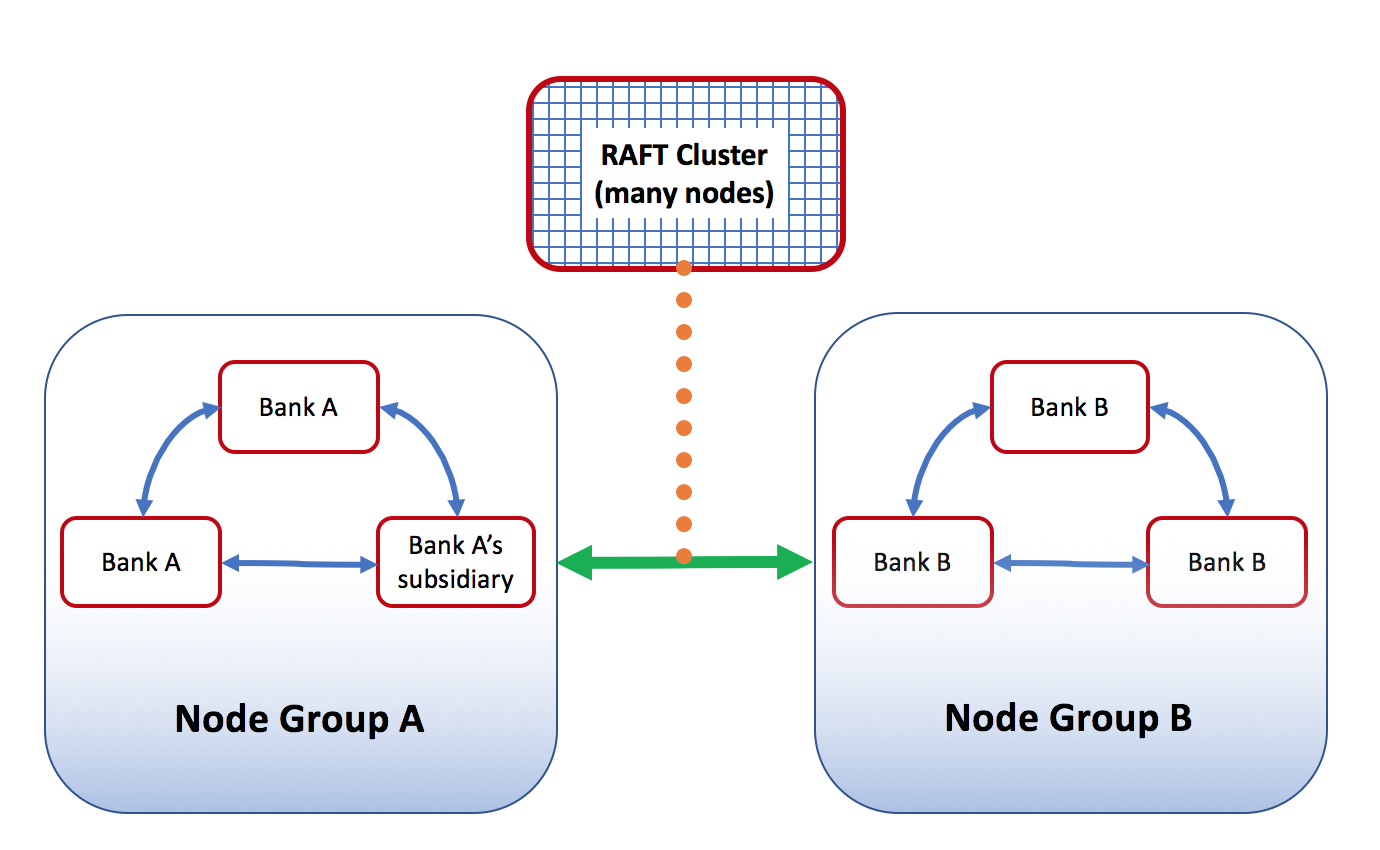
\includegraphics[width=1\textwidth]{notaries.png}
\caption{Cross-group transaction notarisation compared to inner group ones}
\centering
\label{fig:notaries}
\end{figure}
\subsubsection{Transactions}
\label{sub:TP}
We are interested in transaction performance as well. The creation of a transaction could potentially take an arbitrary amount of time - negotiations between the two parties could be carried out (although in our applications these are performed externally and the two participants cannot not end up disagreeing in the system, by definition) or they could be depending on states that do not exist yet. Either way, the performance related to creating transactions is irrelevant - however, we need to explore the performance of transaction transmission (sending and receiving them between participants, committing them). 
\\ \\
\begin{figure}[!htb]
\centering
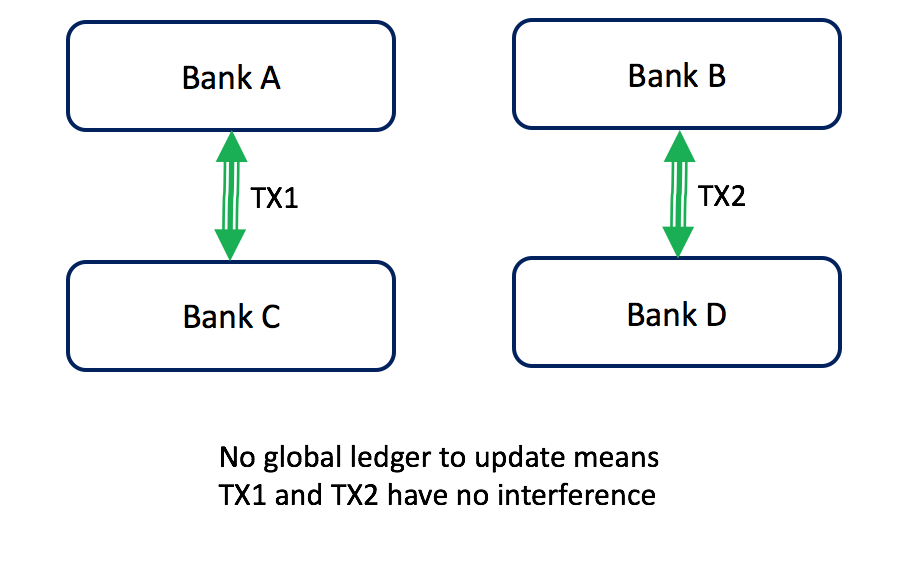
\includegraphics[width=0.6\textwidth]{singular.png}
\caption{Parallel transactions}
\centering
\label{fig:trading}
\end{figure}
\\ \\
Since we have a recommended transaction processing power of 100,000 transactions per second, we want to be able to reach that capacity. Bitcoin currently has the ability to process around 7 transactions per second because they have to be recorded in the global ledger (the chain has to be modified by adding the last verified block). This sequential processing limits its capacities. Corda on the other hand, has a different transmission ideology. If there are only two participants in the transaction, why does everyone need to know about it? Well, they don't. So Corda's peer-to-peer transaction transmission works on a need-to-know basis. Suppose in a system with four banks (A, B, C and D), bank A wants to trade with bank C and bank B wants to trade with bank D. 
\\ \\
\begin{figure}[!htb]
\centering
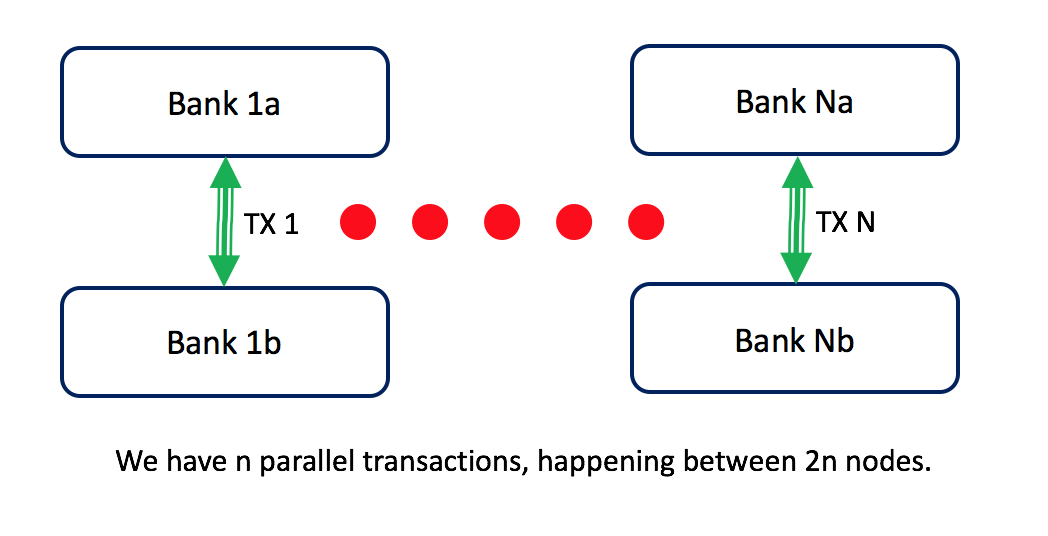
\includegraphics[width=0.6\textwidth]{parallel.png}
\caption{Many independent parallel transactions}
\centering
\label{fig:infinity}
\end{figure}
\\ \\
Like in Figure \ref{fig:trading}, the two transactions are completely independent of each other - there is no ``global ledger" for them to update, therefore they can happen simultaneously. This shows how scalable the system actually is. Since transactions are processed in parallel, without interfering with one another, theoretically there is no speed limit regarding the number of transactions we can have every second (Figure \ref{fig:infinity}). Of course, nodes can transact between them (for example, we can have node 1a transacting with node 5b). Even so, internally, transaction committing does not add any latencies to the process.
\\ \\
Moreover, the fact that there is no theoretical global limit means that an increase in trade volume has no effect on the transacting parties. However, notarising these transactions introduce a bottleneck for processing since they have to be signed before their committing to the node's ledger. But, as mentioned previously, we can have notarising groups - multiple RAFT clusters, for example, that can perform notarisation in parallel. Although the internal node structure has not been optimised for performance yet, some preliminary tests offer some insight into how the notaries perform in practice. Under heavy loads, a one-node, non-validating notary gets around 13 TPS. Given the same conditions, a 5-node non-validating cluster can achieve around 12 TPS (slightly lower because of the database replication) \cite{jira}. These results are coming from tests performed before the initial node optimisations. 
\\ \\
If the latest developments are taken into account, along with the usage of the BFT-Smart library for notarisation, things change for the better. The sustained throughput of raw transaction data for a notary cluster of 1000 clients reaches around 80,000 transactions per second \cite{bftsmart}. The idea is that the more notaries we have, the closer we get to having no global TPS limit. It is also expected that the number of notaries will grow along with the number of members joining the banking consortium. For example, for an initial setting, the same notarising algorithm on a 200-client cluster can achieve around 65,000 TPS.  
\\ \\
One downside to having the parallel transaction messaging happen only between its participants is that there is no global ledger recording all the transactions. This can pose the risk of data loss at the node level, because there are no backups done by the system. Therefore, each node has to individually manage their database backups to protect themselves in case of failure. Although we have the authoritative auditor nodes that register transactions, they might not have all the data required to restore the node's state. One example of this would be internal asset management - for this manipulation, transactions might not be broadcast to the regulators because they pose no interest to them. In this case, there would be no safety net for a node's owner, no other data source that could be used to retrieve lost information. As such, there should be a global requirement for nodes to have their own backups.
\subsection{Security}
\label{sub:Security}
Security is a very important topic to discuss when it comes to the financial world implementing a new system. We have to ensure communications are performed in a secure manner by verifying the identities of the involved parties. We need to guarantee the digital signatures are accurately representing the correct parties and transactions contain all the required signatures for them to be considered ready for committing. For the web interface, we need to mitigate any potential risks that would arise from using unsafe communication channels. And finally, in case of a potential breach of safety, explore the ways in which this can be diminished and eliminated in a fast and inexpensive manner.
\\ \\
Initially, we looked at proving the safety of the system using BAN logic. While it supports reasoning about timeliness (with beliefs expiring over time, as appropriate in our system as well) and it offers a formal structure for the proof, BAN logic has been used for analysing exchange protocols, examining whether the information is trustworthy \cite{banlg}. This is partly useful for our system - we want indeed to verify whether the messages being exchanged are coming from trusted sources, but the way transaction verification is done takes a different form: instead of exchanging a message from party A to party B, we are also adding extra information to the message each time we delegate processing to one of the parties. Even so, at the end of the exchange, after the message can no longer be changed and the two participating parties have verified the contents of the transaction, the notary will perform its check, too! Therefore, we considered BAN logic to be less applicable in this case for a formal proof. Even so, BAN logic would only prove the ideal situation (i.e. the theoretical solution) and not the actual implementation which presents a concern that we would have had to consider.
\subsubsection{Transactions and Notarisation}
Transactions undergo two different types of checks, and we need to understand potential security problems for these verifications. The internal checks are contract-related, each party having access to the details of the transaction and performing its own internal inspections. In the case that the two parties have different Corda binaries that they are running or the flows they are using have different characteristics (which could potentially happen, although not recommended), it is the party's responsibility to examine the contract for all the requirements desired. This is done three-fold: once in the seller, regarding the initial transaction (that only contains the states added by the seller), then in the buyer, after it adds its own states (and at this point the transaction is complete - no additions are to be made; hence, the transaction is converted to an immutable state), then again in the seller to ensure that the final transaction satisfies the initial requirements. The security of this is guaranteed by the digital signatures - every party signs with their private key after they modify the transaction, but they also have to sign \textbf{once the transaction becomes immutable}. This ensures that both parties have seen (and confirmed) the final transaction.
\\ \\
External validation of the transaction, preventing against double-spending or improper usage of states is performed by the notary. The security concern is what happens if the notary gets corrupted or hacked? There are two possibilities: denial of service and rogue signing. The first means that the notary would voluntarily stop signing transactions that are correct and valid, effectively prohibiting any business to take place in the system. The second one would inhibit the role of the notary, making it vulnerable to signing even transactions that are using consumed input states, bad timestamps or that present double-spending. This is identical to what happens in traditional blockchains when an attacker gets control of more than 50\% of the network or manages to compromise the validators. 
\\ \\
For the final planned implementation of Corda, notaries will not be just individual machines (very prone to attacks since the attacker only needs to hack one machine to control its notarisation). A notary will be a logical service composed of multiple machines \cite{attack}. To get the entire validating cluster to behave inappropriately, there are practically two options. The first one is still related to physically hacking the machines (taking control of as many nodes as you need to overthrow the entire network). For a RAFT notary, you could hack only one node and manage to corrupt some traffic that goes through the network but, because of the load-balancing the algorithm does, you would not know which transaction you are affecting. Hence, to be able to pinpoint the specific transaction to corrupt, you need to have 100\% reliability - and this is achieved by corrupting \textbf{all} nodes part of the RAFT cluster. This all has to be done without the attacker getting caught, of course. For the alternative notarisation systems used based on byzantine fault tolerance (BFT) algorithms, an attacker needs to hack more than one node, but not necessarily all of them. The second way of gaining control to the notarisation service is related to persuading (by bribing, threatening or corrupting) the owners of the machines to give over control of the system. However, both cases have a high level of risk attached to them considering they involve the violation of criminal laws. 
\\ \\
Looking at systems that use proof of work, the difference is quite large. Of course, you can still hack the miners and, but you can also get what you want by just spending enough money. There are no legal breaches in this case, because miners have never agreed to any rules (the users assume they are being truthful because of the incentivised system presented by the blockchain). Although a theoretical possibility, miners have actually been reduced to a small number of non-anonymous users with compute farms that enable them to solve the calculations required, meaning that the trust system is very similar to the one presented in Corda. The advantage we have in our system is performance (checks are done more efficiently, faster, and without any information breaches due to the transaction fragmentation preventing the notary from seeing actual transaction details), finality (the proof of work checks only compute an approximation, while the algorithms used by RAFT and BFT give complete results) and cost (spreading a notary cluster on multiple machines is cheaper than having a compute farm in terms of electricity consumed).
\\ \\
Another security benefit encountered in Corda's transactions is related to the need-to-know data sharing. Compared to other implementations that keep a global ledger of public information, Corda distributes the transaction information only to those involved in the contract. Therefore, we are mitigating the risk of accidentally leaking sensitive data to other parties. Hacking one transaction becomes harder since we do not have access to it in all the nodes. Although the attacks could be directed to institutions rather than individual transactions, the permissioning system in place ensures that such attacks would be unsuccessful.
\subsubsection{Web}
\label{sub:websec}
From the point of view of the web interface, the security controls will be put in place for every application developed that hooks into the Corda system. Nodes are already offering security guarantees through the use of HTTPS for connections (mitigating the risk of a man-in-the-middle attack) and the use of certificates for authentication. The certificates will only be released by R3 CEV (the parent company of Corda), adding an extra layer of security for the permissioning. 
\\ \\
The current applications developed on Corda are not using an HTTPS connection, nor are they permissioned with certificates. The reason for this is that it would have been cumbersome to use industry standard techniques for security for such low-level testing. In practice, when the web sites are going to be deployed to actual companies, all the standard safeguards will be in place. 
\subsubsection{Regulations}
\label{sub:reg}
Regulators fully embrace the introduction of a distributed ledger system for trade clearing. This stems from the improved reporting facilities available with such a system, as well as the more effective way of auditing transactions. This fits in well with the requirements of MiFID II, which asks for high quality, complete reporting of trades. However, there are also changes to regulations that will have to be made for this system to be able to replace the traditional banking systems. One of them is related to the legality of transactions - there are currently no laws protecting customers solely on the basis of a digitally signed transaction. However, given that the digital signatures have legal value, it is clear that in the case of a dispute, we could solve it by analysing the contract details and transaction signatures (which would both be legally binding).
\\ \\
One piece of regulation that will change due to the introduction of this system is Regulation T. Clearing and settlement is measured in seconds in Corda, not days. Therefore, Regulation T (the protection measure against counterparty risk), which prohibits trading on money or shares that are unaccounted for (freeriding), would no longer be applicable. This opens a few possibilities for the world of trading. Since cash accounts no longer need to wait for days to trade without posting collateral, we would see a reduction in money lost because of trades that could not be performed due to a lack of settled funds. This could also prompt a merger between the two types of accounts (margin - in which you have an amount of collateral deposited anyway, and cash). The frequency of trades could see a pick up in activity, as well, meaning that the banks' technological infrastructure would have to be stress tested for an increase in trading volume, too. 
\\ \\
Clearing houses would end up having less responsibility, potentially becoming obsolete after more developments in the DLT domain. They could still be used for processes that happen before the transaction gets to our system, such as trade matching and affirmation. Regulations and laws regarding them would see changes as they might be in the same situation as Regulation T - inapplicability. 
\\ \\
The following table (pictured in Figure \ref{fig:summary}) shows a summary of how Corda fulfills the main requirements set out at the beginning of the project.
\begin{figure}[!htb]
\centering
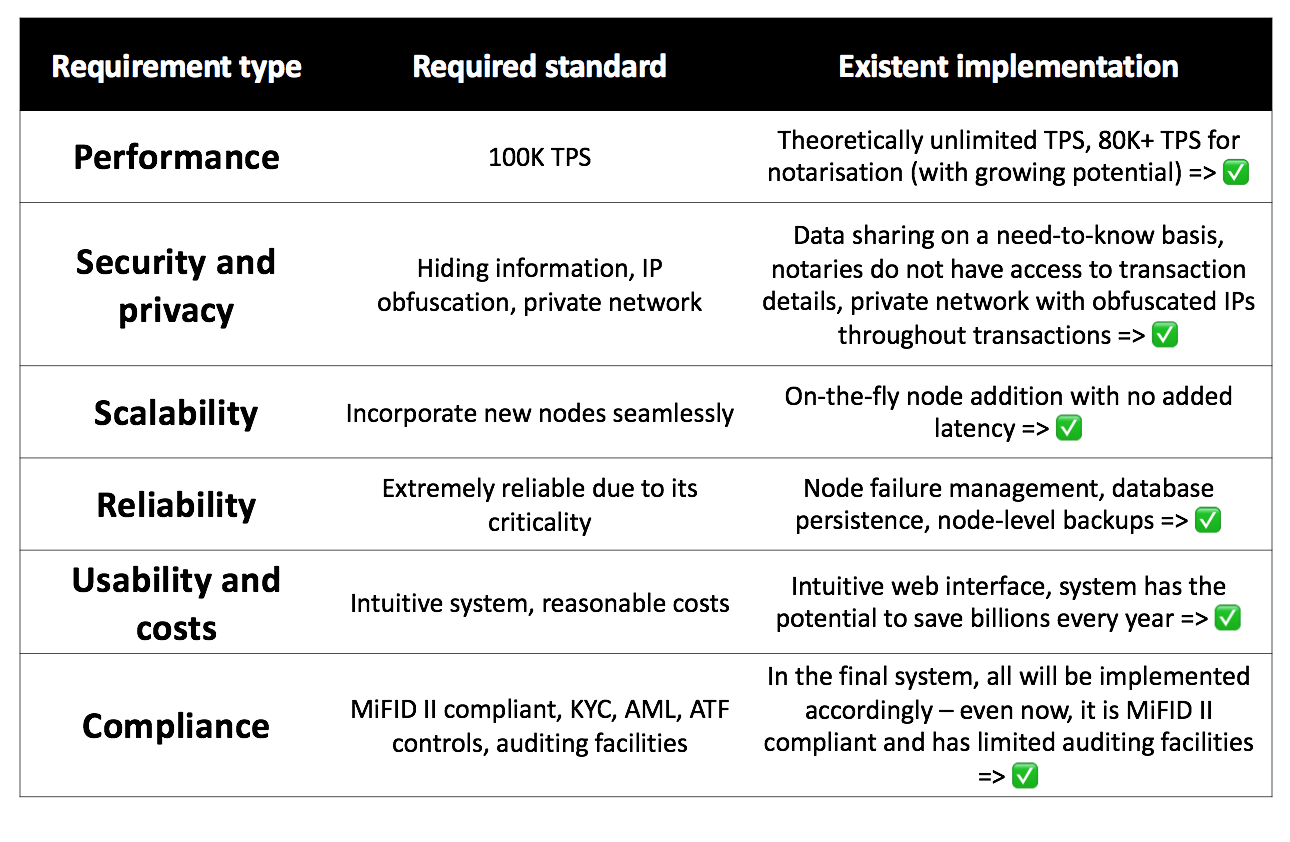
\includegraphics[width=1\textwidth]{reqtble.png}
\caption{Requirement summary}
\centering
\label{fig:summary}
\end{figure}
\newpage

\section{Future work}
\label{sec:Future}
This project offers a glimpse into what the financial world could look like once distributed ledger technology is implemented for its most cumbersome and inefficient tasks. However, there is a long way to go from this work to an actual implementation in the real-world. There are improvements that can be done on this project, as well as developments that can be done on the Corda codebase. 
\\ \\
In this project, the trader demo that features most of the share transfer code could have been developed as an independent CordApp. This would have facilitated the post-deployment management of the plugin and would have isolated this extra piece of behaviour from the core Corda code. Moreover, CordApps are the recommended manner of extending the Corda codebase. The obstacle in doing this from the beginning of the project was the poor structural changes from version M9 to version M10 in the CordApp template. The template was incomplete from the point of view of connections that had to be made (a node running the plugin could not connect to the network map service, for example) and references (you could not implement some pieces of functionality without referring to core Corda code). Moreover, given the extensive changes that were required for the Corda codebase (making the \verb|TwoPartyTradeFlow| implement generic asset exchanges, for example), it was more appropriate to develop share transfers as part of the core implementation rather than an add-on to the core code. Nevertheless, to support the system's modularity, migrating this facility to a proper CordApp is expected.
\\ \\
Moreover, node vault accesses have been simplified for the purposes of share retrieval. In a fully formed system, the accesses in \verb|NodeVaultService| should be more restricted based on ownership and historical movements. This was not convenient at this point because of the limited number of nodes and transactions present in the system. Once this number is increased, the restrictions will make more sense, and this is expected to be implemented in a version released for general consumption.
\\ \\
Identity obfuscation has partially been implemented in this project for share transfers. While the groundwork for this to work has been previously laid down, we decided against focusing on this aspect of the system. It was more important to prove the functional correctness of the flow algorithms by maintaining the same private keys for a node throughout an entire transaction than modifying them midway to provide a secure system. For example, in the \verb|TwoPartyTradeFlow|, the key's only use is to manage and control ownership (not intended to reveal the owner). This is why the key management service derives a unique key from an initial seed meant to provide privacy protection. For a simple share issuance (done by the exchange), we preserve the key obfuscation. However, in the transfer flow, we are using the key to also reveal the identity of the owner in our applications. To note this is only done to better understand the asset exchange and will be modified in the version released for the real-world.
\\ \\
From the point of view of Corda changes that have to be implemented in the future, there are two crucial modifications that need to happen. The first one is modifying the node-vault relation from a one-to-one to a one-to-many. Having more than one vault per node is a natural development, in line with the business case. Although the complexity of the implementation is relatively high, the changes required thereafter to the applications created in this project should be minimal - transactions would either refer to a specific vault (and the underlying network would find the node to which that belongs) or to a node-vault pair instead of just the node, as it currently happens. The node's database would not see major changes - the \verb|VAULT_STATES| table would contain states for all the vaults belonging to one node. To access the states specific to one vault the only modification needed is an extra \textbf{WHERE} clause selecting the correct vault ID.
\\ \\
The second important aspect that has to be fully implemented in Corda to support its business case is the regulatory infrastructure. The example given in this project for auditing is only meant to show the capacity of the system for transaction exploration. However, this should be a built-in feature of Corda, offering auditor nodes more fine-grain details for each transaction and an easier way to dig deep into the transaction history. Again, this feature is also guaranteed to appear in one of the later versions of Corda, especially since some of the infrastructure is already present. For example, we already have the facilities to propagate the details of a transaction to a regulator node, but its implementation is not fully defined. However, as discussed in Section \ref{sub:TheFlows}, we only need to plug in a very small code snippet to broadcast the transaction to the regulator node as well.
\subsection{Industry challenges}
\label{sub:challenges}
One of the main challenges for the industry to implement this system is its usability, cost and maintenance effort. However, to incorporate Corda in the daily routine of a bank is easier than expected. The planned deployment method is to have every bank provided with a Docker image for the component they want. This can be run as a container, offering a minimal maintenance effort for the people involved.
\\ \\
The way to deploy a component would come down to having a Dockerfile that can run a Linux machine and have a JDK installed (along with Kotlin and Gradle). The codebase can either be cloned via git or copied into the contained from the machine. Listing \ref{l:docker} in the Appendix shows how one could have a container set up and running the Corda nodes for one of the applications in a matter of seconds.
\\ \\
Although praised for the improvements DLT can bring to the regulatory world, it also presents a very complex task to the entities that are dealing with legal matters. As an example of how slow regulation is implemented, MiFID II was first released in 2014. After months of modifications, it was finally decided that the date it would enter into effect would be January 2018 \cite{deadlinenew}! Considering the Corda project is not close to its final release, it might take a few years until we see the first implementation of distributed ledger technology being used in a bank.
\newpage
\section{Conclusion}
\label{sec:Conclusion}
Nowadays, fast-paced innovation is a given, especially in the technological areas. But the question arises - why has the financial world not caught up, why is innovation stagnating in this very important sector of our lives? Well, its importance arises from the fact that it deals with our money, the fruit of people's labour. Misplacing or losing cash or exchanging the wrong sums of money would obviously drive people away from a bank, so to enable competition between these institutions, their main feature should be security. Competition prompts the quality of the services to be higher, otherwise there would be no incentive for people staying with one bank. But, this is crux of the problem - \textbf{innovation is not safe}. 
\\ \\
People are adverse to change because there is always a chance something could go wrong. Problems can occur with any upgrade and the results could be disastrous, especially in the banking system. However, the main reason people choose to finally take the step forward is because they have had enough of the current system's problems and shortcomings and the benefits of removing those far outweighs the risk involved with updating it. In my opinion, the financial world has reached a ``settling" point - people are being complacent with the current systems because they are aware of the task at hand if they wanted to change everything (for the better). Will we be able to take the step forward?
\\ \\
Before an answer to that question can be given, we need to revisit all the important requirements for this new, improved banking system: security, performance and regulation.  The technology that is able to tie all these together and produce a high-quality application used commercially is Distributed Ledger Technology. The aim of the project has been to develop a system for trade clearing, settlement and reporting, but not to also use the system for the actual trades, using DLT. We have focused on Corda, which was born out of the desire to create a blockchain-like system for the financial world. To assess Corda's applicability to our requirements, we were prompted to develop a set of extensions and applications that make full use of the available infrastructure. We followed real-world cases which guided us to our main scenario: stock trading between two parties. For this use case, we performed analyses on performance and security, we explored the benefits brought by the system to the regulatory side of trading and we determined the advantages of moving to this system.
\\ \\
We discovered that the system's performance, although the codebase is currently not optimised for it, is in line with the requirements set out by authoritative entities (Central Banks, ESMA). The security used for Corda follows standard practices - and this is enhanced by the use of a semi-private network, to which permissions have to be granted to be able to use it. Security is built into the framework performing transactions through the use of digital signatures. These transactions and the way they are recorded on the ledger are also related to the regulatory aspect that Corda satisfies: complete historical details can be provided to auditor nodes which would assess the legality of transactions.
\\
Using the framework provided and extended, we furthered our proof that Corda is a stable, usable system. We implemented an application which demonstrates the ease of deployment for different entities, as well as the ease of use for the trading facilities. Since these are supported by a graphical interface, we are not expecting traders to perform extensive additional training to be able to operate them. Although there is a shift in trade triggering as opposed to the intuitive way of having the buyer commence a transaction, we need to emphasise that Corda does not deal with any pre-trade details. We are using the system for recording the transaction for posterity and managing the assets of different clients, meaning that this is not (yet) a full trading platform. The second achievement of the project has been to create a random market, where buyers and sellers interact with each other as they would in the real-world. The application tested Corda's messaging systems, performance under heavy loads and the way cash and assets are being traded when many nodes are involved in different processes.
\\ \\
It became clear that using such a technology is the right way to go for the financial world. The long list of benefits has been discussed throughout this project, with the most important ones being that risk and processing times would be slashed in comparison to their current state. However, to be able to achieve this, regulations would have to be implemented to ensure this (or these) new systems are being used with good intentions. Yes, it is a large task for developers to produce and deploy such a system for commercial banks, but it is another big task for regulators to understand the way the industry is shifting and prevent any potential problems that might occur from using such a system.
\\ \\
Several countries have started considering or implementing different solutions related to DLT for their day-to-day business. Most of them are in testing, while others are collaborating for a general-purpose global banking solution. Even so, the timeline for mainstream usage might be longer than some expect. It has been eight years since Bitcoin was released, and it is still being frowned upon by many. Embracing DLT might be a hard step to take for some, disrupting their operations and systems completely. This is accentuated by the scepticism regarding new things, especially when what we are asking is for banks to tread uncharted territory. But it is those banks which will take a leap of faith that will reap the rewards. The world is ready - why shouldn't they be?





\newpage
\bibliography{mybib}
\addcontentsline{toc}{section}{References}
\bibliographystyle{mike}
\newpage
\section*{User Guide} \markboth{{User Guide}}{ }
\addcontentsline{toc}{section}{User Guide}
\label{sec:UG}
For any application, the preamble to running it consists of deploying and starting the nodes. For the building rules of the node structure we are using the \verb|deployNodesWeb| and \verb|deployNodesMkt| tasks of the gradle file from the \verb|samples/trader-demo| package. To deploy the nodes, from the main folder (\verb|corda|), run 
\begin{center}
\verb|./gradlew samples:trader-demo:deployNodesWeb|
\end{center}
(or \verb|Mkt|, as appropriate). To start the nodes, run
\begin{center}
\verb|./samples/trader-demo/build/nodes/runnodes|
\end{center}
This will open up a number of terminal windows, each corresponding to a node (and, in the case of the Web app, a webserver as well). Once the nodes are registered, you can continue with the application.
\subsection*{\textit{Distributed Web Market}}
We have not implemented graphical money issuance - we do not want those who have access to the web site to refill their vaults as they please. We can do this from the terminal, using the \verb|runBuyer| command, though. Each node has a corresponding RPC port (highlighted in the node registration preamble). To self-issue money, run 
\begin{center}
\verb|./gradlew samples:trader-demo:runBuyer -Pamt="\$30000" -Pport=10006|
\end{center}
This command issues \$30,000 to the bank served by port 10006.
For the rest of the application, you would navigate to the address the node is registered to (found in the node registration preamble for the webserver) - this can only be done for market participants, not the notary or Bank of Corda. The two types of participants are: the exchange and the banks. The exchange is able to sell fresh shares to banks - click on the \verb|Sell shares!| button and input the required parameters. The banks are able to sell shares they own - again, click on the \verb|Sell shares!| button and input the parameters for the stock you want to trade.
\subsection*{\textit{Random Market}}
For the random market, there are two types of actions we can perform: issuance and transfers. For the issuance, we generate some sums of money and some shares to all the participants involved in the market. This is done by running
\begin{center}
\verb|./gradlew samples:trader-demo:runRandomI|
\end{center}
It will trigger calls for cash self-issuance and then for fresh shares sales. For the transfers, we randomly perform trades for the given shares by running 
\begin{center}
\verb|./gradlew samples:trader-demo:runRandomT|
\end{center}
This is an infinite loop trying to exchange assets between the different banks in the market. If one of the participants remains without any cash or does not have enough shares, they will automatically be topped up to keep the flow of the application going.
\newpage
\section*{Appendix} \markboth{{Appendix}}{ }
\addcontentsline{toc}{section}{Appendix}
\subsection*{Node addition: code listings}
\lstinputlisting[label = {l:nodebad}, language=Octave, caption = Cumbersome and inefficient deployment of node]{/Users/mikecar/Desktop/Blockchain-dizzy/imgs/nodebad.m}
\newpage
\lstinputlisting[label = {l:nodegood}, language=Octave, caption = On-the-fly node addition (to the existing network map)]{/Users/mikecar/Desktop/Blockchain-dizzy/imgs/nodegood.m}
\newpage
\subsection*{\textit{Random trading} application: code snippets}
\lstinputlisting[label = {l:cashasset}, language=Octave, caption = TraderDemo.kt: code for issuances]{/Users/mikecar/Desktop/Blockchain-dizzy/imgs/ran_iss.m}
\lstinputlisting[label = {l:transfers}, language=Octave, caption = TraderDemo.kt: code for asset transfers]{/Users/mikecar/Desktop/Blockchain-dizzy/imgs/ran_trans.m}
\lstinputlisting[label = {l:sellerT}, language=Octave, caption = TraderDemo.kt: code for one stock trade]{/Users/mikecar/Desktop/Blockchain-dizzy/imgs/runT.m}
Currently, we have the following definition for ports and IPs - this can be made dynamic, both in terms of IPs, port numbers and participants' names. 
\lstinputlisting[label = {l:pi}, language=Octave, caption = TraderDemo.kt: ports definition]{/Users/mikecar/Desktop/Blockchain-dizzy/imgs/comp.m}
\newpage
\subsection*{Dockerfile skeleton}
\lstinputlisting[label = {l:docker}, language=Octave, caption = Dockerfile snippet]{/Users/mikecar/Desktop/Blockchain-dizzy/imgs/docker.m}

\end{document}
%%% Local Variables: 
%%% mode: latex
%%% TeX-master: t
%%% End: 
